\documentclass[mathserif]{beamer}
\usepackage{beamerthemeshadow}
\usepackage{beamerthemesplit}
%\usetheme{shadow}
\usecolortheme{default}
\setbeamertemplate{footline}[frame number]
\useinnertheme[shadow=true]{rounded}
%\setbeamertemplate{footline}{\insertframenumber/\inserttotalframenumber}
%\useoutertheme{infolines}
%\setbeamertemplate{headline}{} % removes the headline that infolines inserts

%\usetheme{boxes}
%\usepackage{amsmass}
%\usepackage{amssymb,amsfonts,url}
\usepackage{amsthm}

\usepackage{algorithm}
\usepackage{algorithmic}

\usepackage{graphicx}
\graphicspath{{Problems/}}

\usepackage{tikz}
\usetikzlibrary{shadows}
\usetikzlibrary{positioning}
\usepackage{verbatim}
\usepackage{pgfplots}
\usepackage{verbatim}
\usetikzlibrary{arrows,shapes}

\definecolor{darkblue}{rgb}{0.2,0.2,0.6}
\definecolor{darkred}{rgb}{0.6,0.1,0.1}
\definecolor{darkgreen}{rgb}{0.2,0.6,0.2}

\usetikzlibrary{shadings,shadows,shapes.arrows}

\usetikzlibrary{calc} 
\makeatletter 
\@namedef{color@3}{blue!20}
\@namedef{color@1}{green!70}   
%\@namedef{color@3}{yellow!50} 
\@namedef{color@2}{orange!90}  
%\@namedef{color@5}{magenta!70} 
%\@namedef{color@6}{yellow!70}    

\newcommand{\graphitemize}[2]{%
\begin{tikzpicture}[every node/.style={align=center}, scale=0.78]  
 \draw[fill=green!5, fill opacity=0.1, green, inner sep=0.05cm, outer sep=0.05cm] (5,0) arc(0:360:5);
 % \draw[fill=white, fill opacity=0.1, white, inner sep=0.05cm, outer sep=0.05cm] (4,0) arc(0:360:4);
%  \shade[ball color=gray!10!] (0,0) coordinate(Hp) circle (.9);
  \node[shape=circle,  minimum size=1.1cm,fill=red!60,font=\Large,outer sep =.15cm,inner sep=.2cm,drop  shadow={ashadow, color=yellow}](ce){#1};  
   % \shade[ball color=blue!20!] (0,0) coordinate($Algorithm$) circle (1.5cm);

\foreach \gritem [count=\xi] in {#2}  {\global\let\maxgritem\xi}  
\foreach \gritem [count=\xi] in {#2}
{% 
\pgfmathtruncatemacro{\angle}{90+360/\maxgritem*\xi}
\edef\col{\@nameuse{color@\xi}}
\node[shape=circle,
     ultra thick,
     draw=white,
     fill opacity=1,
     drop  shadow={ashadow, color=blue!60},
     fill=\col,outer sep=0.25cm,        
     minimum size=2cm] (satellite-\xi) at (\angle:5cm) {\gritem };
     \draw[line width=0.25cm,-latex, \col] (ce) -- (satellite-\xi);
     }%
% \draw[violet, fill=violet!10] (4,0) arc(0:360:4);
\end{tikzpicture}  
}%



\newcommand*{\tikzarrow}[2]{%
  \tikz[
    baseline=(A.base),             % Set baseline to the baseline of node content
    font=\footnotesize\sffamily    % Set fontsize of the node content
  ]
  \node[
    single arrow,                  % Shape of the node
    single arrow head extend=2pt,  % Actual width of arrow head
    draw,                          % Draw the node shape
    inner sep=2pt,                 % Separation between node content and node shape
    top color=white,               % Shading color on top of node
    bottom color=#1,               % Shading color on bottom of node
    drop shadow                    % Draw a shadow
  ] (A) {#2};%
}


\def\arrow{
  (10.05:1.1) -- (6.05:1) arc (6.05:120:1) [rounded corners=0.5] --
  (120:0.9) [rounded corners=1] -- (130:1.1) [rounded corners=0.5] --
  (120:1.3) [sharp corners] -- (120:1.2) arc (120:5.25:1.2)
  [rounded corners=1] -- (10.05:1.1) -- (6.05:1) -- cycle
}

\tikzset{
  ashadow/.style={opacity=.25, shadow xshift=0.07, shadow yshift=-0.07},
}

\def\arrows[#1]{         
  \begin{scope}[scale=#1]
    \draw[color=darkred, drop  shadow={ashadow, color=red!60!black}] \arrow;

    \draw[color=darkgreen, bottom color=green!90!black, top color=green!60,   drop shadow={ashadow, color=green!60!black}] [rotate=120] \arrow;

    \draw[color=darkblue, right color=blue, left color=blue!60,   drop shadow={ashadow, color=blue!60!black}] [rotate=240] \arrow;

    % to hide the green shadow
    \draw[color=darkred, left color=red, right color=red!60] \arrow;
  \end{scope}
}

\tikzstyle{vertex}=[circle,fill=black!25,draw,minimum size=20pt,inner sep=0pt]
\tikzstyle{middlevertex}=[circle,fill=black!25,draw,minimum size=15pt,inner sep=0pt]
\tikzstyle{smallvertex}=[circle,fill=black!25,draw,minimum size=10pt,inner sep=0pt]
\tikzstyle{middlesmallvertex}=[circle,fill=black!25,draw,minimum size=11pt,inner sep=0pt]
\tikzstyle{tinyvertex}=[circle,fill=black!25,draw,minimum size=5pt,inner sep=0pt]
\tikzstyle{selected vertex} = [vertex, draw,fill=yellow!24]
\tikzstyle{blue smallvertex} = [smallvertex, draw,fill=blue]
\tikzstyle{red smallvertex} = [smallvertex, draw,fill=yellow]
\tikzstyle{edge} = [draw,thick,->]
\tikzstyle{undirectededge} = [draw,thick]
\tikzstyle{weight} = [font=\small]
\tikzstyle{selected edge} = [draw,line width=3pt,-,red!50]
\tikzstyle{ignored edge} = [draw,line width=3pt,-,black!20]
\tikzstyle{squarednode}=[draw, fill=blue!20, thick, minimum size=5mm]
\tikzstyle{roundnode}=[circle, draw, fill=blue!20, thick, minimum size=5mm]




%\usepackage{CJK}
%\usepackage{pinyin}

%    \begin{figure}
%        \centering
%        \includegraphics[width=0.8\textwidth]{newGeneRep.eps}
%    \end{figure}

% \begin{figure}%
%   \begin{center}%
%     \begin{minipage}{0.70\textwidth}%
%      \includegraphics[width=1.0\textwidth]{comp25000.eps}%
%     \end{minipage}%
%     \begin{minipage}{0.30\textwidth}
%      \includegraphics[width=1.0\textwidth]{comparelabel.eps}%
%     \end{minipage}%
%   \end{center}
% \end{figure}

% \begin{table}
%   {\begin{tabular}{l|rrr}\hline
%       & vlticolumn{3}{c}{Actual number of DCJ operations}\\
%       \# genes &\# genes $\times 1$&\# genes $\times 2$&\# genes  $\times 3$ \\
% \hline
%      (a)~25,000 & 0.5\% ~~&  0.9\% ~~& 1.7\%~~\\
%       (b)~10,000 & 0.8\%~~ &  1.4\% ~~& 2.7\%~~\\
%      (c)~ 1,000 & 2.7\%~~ & 4.7\%~~ & 14.7\%~~\\ \hline
%     \end{tabular}} {}%
% \end{table}

% \begin{eqnarray}
% T(n) &=&  \sum_{i=1}^n C_i \\
%      &=&  \# PUSH + \#POP \\
%      &<& 2\times \#PUSH \\
%      &<& 2n \\
% \end{eqnarray}

% \[ 
% \begin{matrix}
% \begin{pmatrix}
% C_{11} & C_{12} \\ 
% C_{21} & C_{22} 
% \end{pmatrix}
% =
% \begin{pmatrix}
% A_{11} & A_{12} \\ 
% A_{21} & A_{22}  
% \end{pmatrix}
% 
% \begin{pmatrix}
% B_{11} & B_{12} \\ 
% B_{21} & B_{22}  
%  
% \end{pmatrix}
%     
%    \end{matrix}
% \]
% 
% 
% \begin{eqnarray}
%  C_{11} &=& (A_{11}\times B_{11}) + (A_{12} \times B_{21}) \\
% C_{12} &=& (A_{11}\times B_{12}) + (A_{12} \times B_{22}) \\
% C_{21} &=& (A_{21}\times B_{11}) + (A_{22} \times B_{21}) \\
% C_{22} &=& (A_{21}\times B_{12}) + (A_{22} \times B_{22}) 
% \end{eqnarray}
% \begin{figure}%
%      \begin{minipage}{0.32\textwidth}%
%       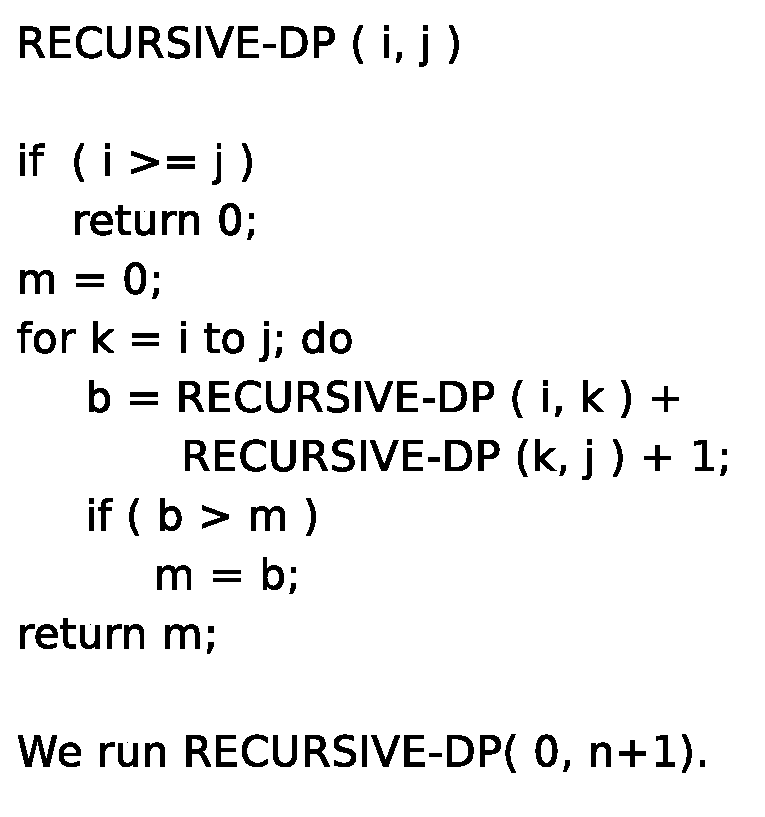
\includegraphics[width=1.0\textwidth]{L7-intervalschedulingdpalgo.eps}%
%      \end{minipage}%
%  \quad
%      \begin{minipage}{0.30\textwidth}
%       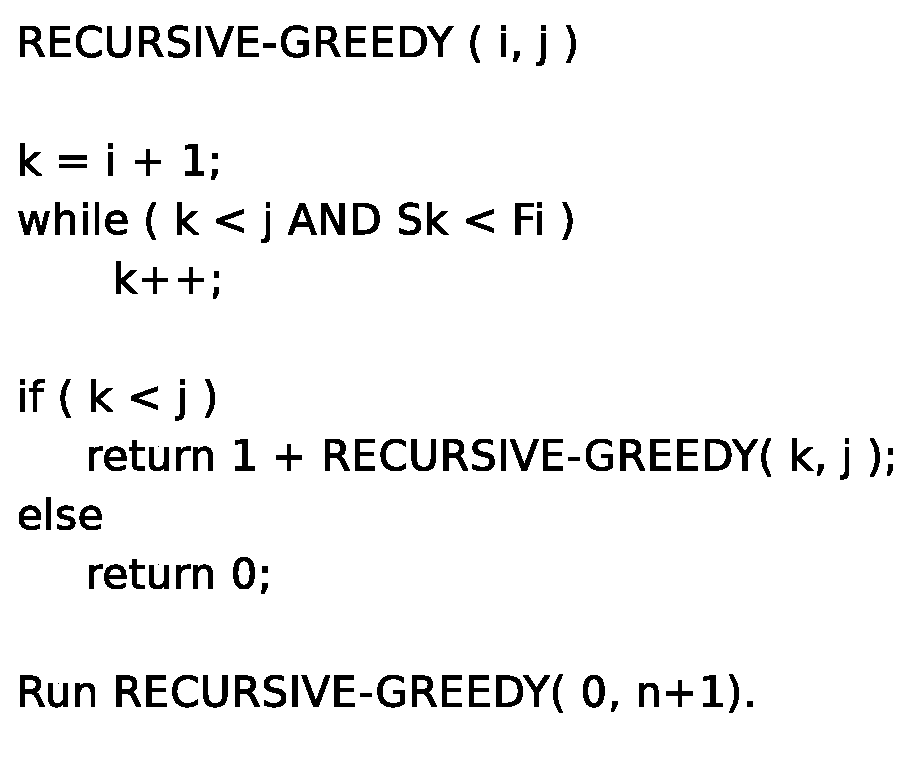
\includegraphics[width=1.0\textwidth]{L7-intervalschedulinggreedyalgo.eps}%
%      \end{minipage}%
%  \quad
%       \begin{minipage}{0.25\textwidth}
%       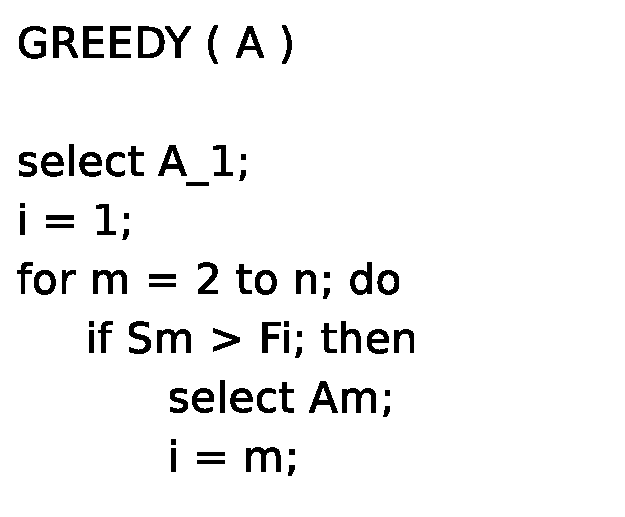
\includegraphics[width=1.0\textwidth]{L7-intervalschedulinggreedyalgo2.eps}%
%      \end{minipage}%
% 
%  \end{figure}

\title{CS711008Z  Algorithm Design and Analysis }
\subtitle{ Lecture 10. {\sc Assignment}, {\sc MaximumMatching} and {\sc MaximumWeightedMatching} problems
\footnote{The slides are made based on Kuhn1955, Egerv\'{a}ry1931, Konig1931, von Neumann1950, Edmonds1965a/b, Munkers1957, and Berge1957.} 
}
\author{Dongbo Bu } 
\institute{ {\small Institute of Computing Technology \\ 
Chinese Academy of Sciences, Beijing, China}}

\date{}

\begin{document}
%\begin{CJK}{UTF8}{cyberbit}



\frame{\titlepage}

\frame{
\frametitle{Outline}
\begin{itemize}
\item {\sc Assignment} problem; 
\item {\sc MaximumMatching} in bi-partite graph: \textcolor{black}{alternating} paths; Berge's lemma, K\"{o}nig's theorem; Hopcroft-Karp algorithm; ILP formulation; 
\item {\sc MaximumWeightedMatching} in bi-partite graph: Egerv\'{a}ry's idea; Hungarian algorithm; 
\item {\sc MaximumMatching} in general graph: Blossom algorithm; 
\item {\sc MaximumWeightedMatching} in general graph;
%: Hungarian algorithm; 
%%problem: {\sc Ford-Fulkerson} algorithm, {\sc MaxFlow-MinCut} theorem; 
%\item A duality explanation of {\sc Ford-Fulkerson} algorithm and {\sc MaxFlow-MinCut} theorem;
%\item Scaling technique to improve {\sc Ford-Fulkerson} algorithm;
%\item Solving the dual problem: Push-Relabel algorithm; 
%%\item Connection with divide-and-conquer technique; 
%\item Extensions of {\sc MaximumFlow} problem: lower bound of capacity, multiple sources $\&$ multiple sinks, indirect graph; 
%\item Applications of network flow: {\sc BipartiteMatching}, {\sc ProteinDomainParsing}, {\sc BaseballElimination}, {\sc ImageSegmentation}, {\sc SurveyDesign}, {\sc FlightScheduling};
\end{itemize}

%Remarks: \\
%\begin{enumerate}
% \item The LP model of network flow problem can \textcolor{red}{automatically generate integral solution.}
% \item The powerful \textcolor{red}{scaling} technique can significantly reduce time-complexity from $O(mC)$ to $O(m^2 \log C)$. 
%%  \item 
%\end{enumerate}
}



\frame{
	\frametitle{A brief history}
	
	\begin{itemize}
		\item In 1784, G. Monge studied the {\sc assignment} problem. 
		\item In 1916,  D. K\"{o}nig studied the matching problem for bi-partite graphs.
		\item In 1931, J. Egerv\'{a}ry studied the weighted version of the matching problem. 
		\item In 1950, von Neumann proved the equivalence between {\sc assignment} problem and two players' {\sc zero-sum} game. 
		\item In 1955, H. Kuhn proposed the {\sc Hungarian} algorithm.
		\item In 1957, Munkres gave a analysis of the {\sc Hungarian} algorithm. 
		\item In 1964,  J. Edmonds proposed the {\sc Blossum} algorithm for matching in general graph (together with the concept of ``efficient algorithms").  		
	\end{itemize}
}


\frame{
	\frametitle{A brief history}
 \begin{figure}%
   \begin{center}%
     \begin{minipage}{0.2\textwidth}%
      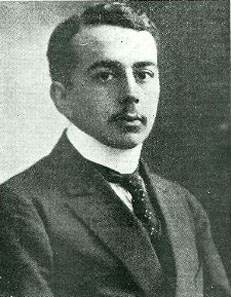
\includegraphics[width=1.0\textwidth]{Konig.jpg}%
     \end{minipage}%
     \quad
     \begin{minipage}{0.2\textwidth}
      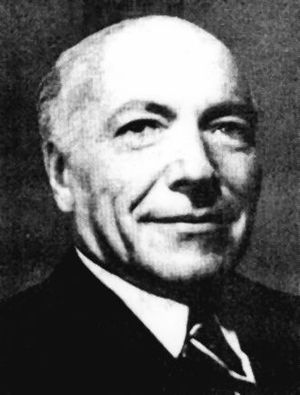
\includegraphics[width=1.0\textwidth]{Egervary.jpg}%
     \end{minipage}%
     \quad
     \begin{minipage}{0.2\textwidth}
      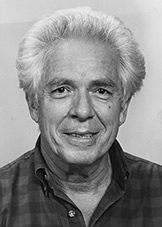
\includegraphics[width=1.0\textwidth]{Kuhn.jpg}%
     \end{minipage}%     
     \quad
     \begin{minipage}{0.2\textwidth}
      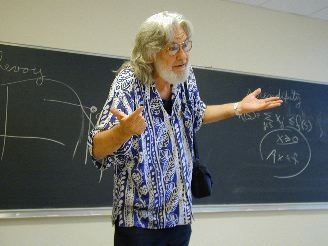
\includegraphics[width=1.0\textwidth]{Edmonds.jpg}%
     \end{minipage}%     

   \end{center}
   \caption{D. K\"{o}nig, J. Egerv\'{a}ry,  H. Kuhn, and J. Edmonds}
 \end{figure}

}


\frame{
	\begin{block}{}
		 1. {\sc Assignment} problem and {\sc MaximumMatching} in bi-partite graph
	\end{block}
}


\frame{
	\frametitle{ {\sc Assignment} problem in terms of matrix  } 
	
%	\begin{itemize}
%		\item Practical problem 
			\begin{itemize}
				\item Let's consider the following {\sc assignment} problem: there are three individuals (denoted as $I=\{I_1, I_2, I_3\}$), and three jobs $J=\{J_1, J_2, J_3\}$. Any individual might qualify one or more jobs. This information can be presented effectively by  a \textcolor{red}{\bf qualification matrix}, where $q_{ij}=1$ if $I_i$ qualifies $J_j$, and $q_{ij}=0$ otherwise. For example,  

\[
Q=\left[ \begin{array}{ccc}
0 & \textcolor{red}{1} & 0 \\
\textcolor{red}{1} & 1 & 1\\
0 & 1 & \textcolor{red}{1} 
 \end{array} \right]
\]

%\begin{figure}
%    \begin{tikzpicture}[scale=1., auto,swap]
%    % Draw a 7,11 network
%    % First we draw the vertices
%    \node at (0, 0.5) {$I$};
%    \node at (2, 0.5) {$J$};
%    
%    \foreach \pos/\name/\label in {{(0,0)/I1/I_1}, {(0,-1)/I2/I_2}, {(0,-2)/I3/I_3}, {(2, 0)/J1/J_1}, {(2, -1)/J2/J_2}, {(2, -2)/J3/J_3}}
%        \node[middlesmallvertex,draw=black, fill=blue!20] (\name) at \pos {\tiny $\label$};
%  
%    % Connect vertices with edges and draw weights
%   \foreach \source/ \dest /\weight in {I1/J2/{}, I2/J1/{}, I2/J2/{}, I2/J3/{}, I3/J2/{}, I3/J3/{}}
%          \path[undirectededge] (\source) -- node[weight] {$\weight$} (\dest);
%%       \draw[dashed, ->] (0,0) arc  (120:60:2);
% 
% \node at (-3, -1) {$Q=\left[ \begin{array}{ccccc}
%1 & 2 & 3 & 4 &5\\
%1 & 2 & 3 & 4 &5\\
%1 & 2 & 3 & 4 &5\\
%1 & 2 & 3 & 4 &5
% \end{array} \right]
%$}; 
% 
%   \end{tikzpicture}
%\end{figure}					
				\item Question:  what is the largest number of jobs that can be assigned to qualified individuals (with at most one job assigned to an individual)? In other words, what is the largest number of $1$'s that can be chosen, with no two in the same row or column?   
				\footnote{ This problem was regarded as the most degenerate case of the {\sc Transporation} problem, and a relative of the traveling salesman problem. }

\end{itemize}

%	\end{itemize}
}

\frame{
	\frametitle{ {\sc Assignment} problem in terms of graph theory} 

\begin{itemize}
\item The  {\sc Assignment} problem can be described in the language of graph theory, where nodes represent individuals and jobs, and edges represent qualification. 
\begin{figure}
    \begin{tikzpicture}[scale=1., auto,swap]
    % Draw a 7,11 network
    % First we draw the vertices
    \node at (0, 0.5) {$I$};
    \node at (2, 0.5) {$J$};
    
    \foreach \pos/\name/\label in {{(0,0)/I1/I_1}, {(0,-1)/I2/I_2}, {(0,-2)/I3/I_3}, {(2, 0)/J1/J_1}, {(2, -1)/J2/J_2}, {(2, -2)/J3/J_3}}
        \node[middlesmallvertex,draw=black, fill=blue!20] (\name) at \pos {\tiny $\label$};
  
    % Connect vertices with edges and draw weights
   \foreach \source/ \dest /\weight in {I1/J2/{}, I2/J1/{}, I2/J2/{}, I2/J3/{}, I3/J2/{}, I3/J3/{}}
          \path[undirectededge] (\source) -- node[weight] {$\weight$} (\dest);
%       \draw[dashed, ->] (0,0) arc  (120:60:2);
   \foreach \source/ \dest /\weight in {I1/J2/{}, I2/J1/{}, I3/J3/{}}
          \path[undirectededge, red, ultra thick] (\source) -- node[weight] {$\weight$} (\dest);
 
 \node at (-3, -1) {$
Q=\left[ \begin{array}{ccc}
0 & \textcolor{red}{1} & 0 \\
\textcolor{red}{1} & 1 & 1\\
0 & 1 & \textcolor{red}{1} 
 \end{array} \right]
$}; 
 
   \end{tikzpicture}
\end{figure}					

\item Thus, the {\sc Assignment} problem essentially attempts to find  
	{\sc MaximumMatching} in bi-partite graph.  


	\begin{block}{}
			  {\bf INPUT}:  a bipartite graph $G= (L\cup R, E)$;\\ 
			 {\bf OUTPUT}: the \textcolor{red}{\bf  matching} $M$ with maximum cardinality. Here, a \textcolor{red}{\bf matching}, also known as \textcolor{red}{\bf independent edge set},  refers to a set of  \textcolor{blue}{\bf edges without common vertices}. 
	\end{block}	
\end{itemize}
	


}

\frame{
	\frametitle{  {\sc MaximumMatching} in bi-partite graph } 
	\begin{itemize}
		\item 
	We will talk about the following issues. 
		\begin{itemize}
			\item The {\sc alternating path} technique
			\item  Berge's lemma on optimality 
			\item  Maximum-flow approach and Hopcroft-Karp algorithm 
			\item  Linear program formulation and dual problem
			\item  K\"{o}nig's theorem: {\sc MaxMatching} and {\sc MinVertexCover} (and Hall's theorem)
		\end{itemize}
	\end{itemize}
}


\frame{
	\begin{block}{}
	1.1 Finding {\sc MaxMatching} using alternating paths 
	\end{block}
}

\frame{
\frametitle{Applying the general {\sc Improvement} strategy } 

\begin{algorithmic}[1]
\STATE $\mathbf{M=M_0}$; //set initial solution;
\WHILE{  \texttt{TRUE} }
\STATE $\mathbf{M}=${\sc Improve}$(\mathbf{M})$; //move towards optimum;  
\IF { {\sc Stopping}$(\mathbf{M})$}  
\STATE break;
\ENDIF
\ENDWHILE
\RETURN $\mathbf{M}$;
\end{algorithmic}

\begin{itemize}
	\item The basic idea is to increase cardinality of matching step by step. 
	\item  It is trivial to set initial solution, e.g., a null matching. Thus the remaining are how to improve matching and when to stop (i.e., optimality condition). 
\end{itemize}

}

\frame{
\frametitle{How to improve a matching? A simple way} 
\begin{itemize}
	\item It is clear that we can increase matching by simply placing an unassigned individual in  an unassigned job that the individual qualifies. 
			\begin{figure}
\begin{tikzpicture}[scale=1., auto,swap]

    % Draw a 7,11 network
    % First we draw the vertices
    \def\dx{-8}; 
    \foreach \pos/\name/\label in {{(0+\dx,0)/I1/I_1}, {(0+\dx,-1)/I2/I_2}, {(0+\dx,-2)/I3/I_3}, {(2+\dx, 0)/J1/J_1}, {(2+\dx, -1)/J2/J_2}, {(2+\dx, -2)/J3/J_3}}
        \node[middlesmallvertex,draw=black, fill=blue!20] (\name) at \pos {\tiny $\label$};
  
    % Connect vertices with edges and draw weights
  \foreach \source/ \dest /\weight in {I1/J2/{}, I2/J1/{}, I2/J2/{}, I2/J3/{}, I3/J2/{}, I3/J3/{}}
          \path[undirectededge] (\source) -- node[weight] {$\weight$} (\dest);
%       \draw[dashed, ->] (0,0) arc  (120:60:2);

    % Connect vertices with edges and draw weights
%  \foreach \source/ \dest /\weight in {I2/J2/{}}
%          \path[undirectededge, red, ultra thick] (\source) -- node[weight] {$\weight$} (\dest);
%%       \draw[dashed, ->] (0,0) arc  (120:60:2);
\node[ultra thick] at (1+\dx, -2.5) {$M$}; 

\draw[->, blue, ultra thick] (2+\dx + 0.6, -1) -- (2+\dx+1.3, -1); 

    % Draw a 7,11 network
    % First we draw the vertices
    \def\dx{-4}; 
    \foreach \pos/\name/\label in {{(0+\dx,0)/I1/I_1}, {(0+\dx,-1)/I2/I_2}, {(0+\dx,-2)/I3/I_3}, {(2+\dx, 0)/J1/J_1}, {(2+\dx, -1)/J2/J_2}, {(2+\dx, -2)/J3/J_3}}
        \node[middlesmallvertex,draw=black, fill=blue!20] (\name) at \pos {\tiny $\label$};
  
    % Connect vertices with edges and draw weights
  \foreach \source/ \dest /\weight in {I1/J2/{}, I2/J1/{}, I2/J2/{}, I2/J3/{}, I3/J2/{}, I3/J3/{}}
          \path[undirectededge] (\source) -- node[weight] {$\weight$} (\dest);
%       \draw[dashed, ->] (0,0) arc  (120:60:2);

    % Connect vertices with edges and draw weights
  \foreach \source/ \dest /\weight in {I2/J2/{}}
          \path[undirectededge, red, ultra thick] (\source) -- node[weight] {$\weight$} (\dest);
%       \draw[dashed, ->] (0,0) arc  (120:60:2);

\node[ultra thick] at (1+\dx, -2.5) {$M'$}; 

\draw[->, blue, ultra thick] (2+\dx + 0.6, -1) -- (2+\dx+1.3, -1); 


    % Draw a 7,11 network
    % First we draw the vertices
\def\dx{0};
    \foreach \pos/\name/\label in {{(0,0)/I1/I_1}, {(0,-1)/I2/I_2}, {(0,-2)/I3/I_3}, {(2, 0)/J1/J_1}, {(2, -1)/J2/J_2}, {(2, -2)/J3/J_3}}
        \node[middlesmallvertex,draw=black, fill=blue!20] (\name) at \pos {\tiny $\label$};
  
    % Connect vertices with edges and draw weights
  \foreach \source/ \dest /\weight in {I1/J2/{}, I2/J1/{}, I2/J2/{}, I2/J3/{}, I3/J2/{}, I3/J3/{}}
          \path[undirectededge] (\source) -- node[weight] {$\weight$} (\dest);
%       \draw[dashed, ->] (0,0) arc  (120:60:2);

    % Connect vertices with edges and draw weights
  \foreach \source/ \dest /\weight in {I2/J2/{},  I3/J3/{}}
          \path[undirectededge, red, ultra thick] (\source) -- node[weight] {$\weight$} (\dest);
%       \draw[dashed, ->] (0,0) arc  (120:60:2);
\node[ultra thick] at (1+\dx, -2.5) {$M''$}; 


   \end{tikzpicture}
\end{figure}
		
	\item Note that the matching $M''$ cannot be further improved. In fact, $M''$ is a \textcolor{red}{\bf maximal matching} (also called \textcolor{blue}{\bf complete} by H. Kuhn) rather than \textcolor{red}{\bf maximum matching}.  A set is \textcolor{red}{\bf maximal} w.r.t. a property if it has the property but is not properly contained in any set that has this property. 
	\end{itemize}
}


\frame{
\frametitle{A more effective  improvement strategy:  {\sc Transfer} } 
\begin{itemize}
	\item Note that the error is the assignment of $J_2$ to $I_2$. Thus, we can move $I_2$ from $J_2$ to $J_1$, and assign $J_1$ to $I_2$, which increases the matching by one. 
	\item This operation (called  {\sc Transfer} by H. Kuhn) can be implemented using \textcolor{red}{\bf augmenting path}. 
	
\begin{figure}
\begin{tikzpicture}[scale=1., auto,swap]
    % Draw a 7,11 network
    % First we draw the vertices
    \foreach \pos/\name/\label in {{(0,0)/I1/I_1}, {(0,-1)/I2/I_2}, {(0,-2)/I3/I_3}, {(2, 0)/J1/J_1}, {(2, -1)/J2/J_2}, {(2, -2)/J3/J_3}}
        \node[middlesmallvertex,draw=black, fill=blue!20] (\name) at \pos {\tiny $\label$};
  
    % Connect vertices with edges and draw weights
  \foreach \source/ \dest /\weight in {I1/J2/{}, I2/J1/{}, I2/J2/{}, I2/J3/{}, I3/J2/{}, I3/J3/{}}
          \path[undirectededge] (\source) -- node[weight] {$\weight$} (\dest);
%       \draw[dashed, ->] (0,0) arc  (120:60:2);

    % Connect vertices with edges and draw weights
  \foreach \source/ \dest /\weight in {I2/J2/{},  I3/J3/{}}
          \path[undirectededge, red, ultra thick] (\source) -- node[weight] {$\weight$} (\dest);
%       \draw[dashed, ->] (0,0) arc  (120:60:2);

\draw[ultra thick, ->, blue]  (2.7, -1) -- (3.3,-1); 

    \foreach \pos/\name/\label in {{(4,0)/I1/I_1}, {(4,-1)/I2/I_2}, {(4,-2)/I3/I_3}, {(6, 0)/J1/J_1}, {(6, -1)/J2/J_2}, {(6, -2)/J3/J_3}}
        \node[middlesmallvertex,draw=black, fill=blue!20] (\name) at \pos {\tiny $\label$};
  
    % Connect vertices with edges and draw weights
  \foreach \source/ \dest /\weight in {I1/J2/{}, I2/J1/{}, I2/J2/{}, I2/J3/{}, I3/J2/{}, I3/J3/{}}
          \path[undirectededge] (\source) -- node[weight] {$\weight$} (\dest);
%       \draw[dashed, ->] (0,0) arc  (120:60:2);

    % Connect vertices with edges and draw weights
  \foreach \source/ \dest /\weight in {I1/J2/{}, I2/J1/{}, I3/J3/{}}
          \path[undirectededge, red, ultra thick] (\source) -- node[weight] {$\weight$} (\dest);
%       \draw[dashed, ->] (0,0) arc  (120:60:2);

   \end{tikzpicture}
\end{figure}
\end{itemize}

}


\frame{
	\frametitle{Improvement using augmenting paths} 
\begin{Definition}[{\sc Alternating path} and {\sc augmenting path}]
	An {\sc alternating path} w.r.t.  a matching $M$ contains edges alternatively in $M$ and  $E-M$.   
	 An alternating path starting from and ending at unmatched vertex is denoted as {\sc augmenting path}, e.g. $I_1 \rightarrow J_2 \rightarrow I_2 \rightarrow J_1$. 
\end{Definition}
	
	\begin{figure}
\begin{tikzpicture}[scale=1., auto,swap]
    % Draw a 7,11 network
    % First we draw the vertices
    \foreach \pos/\name/\label in {{(0,0)/I1/I_1}, {(0,-1)/I2/I_2}, {(0,-2)/I3/I_3}, {(2, 0)/J1/J_1}, {(2, -1)/J2/J_2}, {(2, -2)/J3/J_3}}
        \node[middlesmallvertex,draw=black, fill=blue!20] (\name) at \pos {\tiny $\label$};
  
    % Connect vertices with edges and draw weights
  \foreach \source/ \dest /\weight in {I1/J2/{}, I2/J1/{}, I2/J2/{}, I2/J3/{}, I3/J2/{}, I3/J3/{}}
          \path[undirectededge] (\source) -- node[weight] {$\weight$} (\dest);
%       \draw[dashed, ->] (0,0) arc  (120:60:2);

    % Connect vertices with edges and draw weights
  \foreach \source/ \dest /\weight in { I3/J3/{}}
          \path[undirectededge, red, ultra thick] (\source) -- node[weight] {$\weight$} (\dest);
%       \draw[dashed, ->] (0,0) arc  (120:60:2);
	
  \node[ultra thick] at (1, -2.5) {$M$};
	

%\draw[ultra thick, ->, blue]  (2.7, -1) -- (3.3,-1); 

    \foreach \pos/\name/\label in { {(4,-1)/I2/I_2}, {(4,-2)/I3/I_3}, {(6, -1)/J2/J_2}, {(6, -2)/J3/J_3}}
        \node[middlesmallvertex,draw=black, fill=blue!20] (\name) at \pos {\tiny $\label$};
  
    % Connect vertices with edges and draw weights
  \foreach \source/ \dest /\weight in { I2/J3/{}, I3/J2/{}, I3/J3/{}}
          \path[undirectededge] (\source) -- node[weight] {$\weight$} (\dest);
%       \draw[dashed, ->] (0,0) arc  (120:60:2);

    % Connect vertices with edges and draw weights
  \foreach \source/ \dest /\weight in { I3/J3/{}}
          \path[undirectededge, red, ultra thick] (\source) -- node[weight] {$\weight$} (\dest);
%       \draw[dashed, ->] (0,0) arc  (120:60:2);

 \node[ultra thick] at (1+4, -2.5) {augmenting path 1};


    \foreach \pos/\name/\label in { {(8,-1)/I2/I_2},  {(10, -1)/J2/J_2}}
        \node[middlesmallvertex,draw=black, fill=blue!20] (\name) at \pos {\tiny $\label$};

  \foreach \source/ \dest /\weight in { I2/J2/{}}
          \path[undirectededge,  thick] (\source) -- node[weight] {$\weight$} (\dest);

 \node[ultra thick] at (1+4+4, -2.5) {augmenting path 2};


   \end{tikzpicture}
\end{figure}

\begin{itemize}
	\item Note that an augmenting path w.r.t. $M$ has odd number of edges, containing one more edge in $E-M$ than that in $M$. 
\end{itemize}


} 


\frame{
	\frametitle{Improving matching $M$ through calculating $M\oplus P$} 
\begin{itemize}
	\item The \textcolor{blue}{\bf symmetric difference} of a matching $M$ and  an  augmenting path $P$ leads  to \textcolor{red}{\bf an improved matching}. 
\end{itemize}

\begin{Lemma}[]
For an augmenting path $P$ w.r.t. a matching $M$,  the \textcolor{blue}{\bf symmetric difference} $M\oplus P=(M-P)\cup(P-M)$  exchanges the edges in $P\cap M$ and those  in $P\cap \overline{M}$, forming a new matching with one more pair, i.e., 
$| M\oplus P | = |M| + 1$. 
\end{Lemma}

	\begin{figure}
\begin{tikzpicture}[scale=1., auto,swap]

    % Draw a 7,11 network
    % First we draw the vertices
    \def\dx{-4};
    \foreach \pos/\name/\label in {{(0+\dx,0)/I1/I_1}, {(0+\dx,-1)/I2/I_2}, {(0+\dx,-2)/I3/I_3}, {(2+\dx, 0)/J1/J_1}, {(2+\dx, -1)/J2/J_2}, {(2+\dx, -2)/J3/J_3}}
        \node[middlesmallvertex,draw=black, fill=blue!20] (\name) at \pos {\tiny $\label$};
  
    % Connect vertices with edges and draw weights
  \foreach \source/ \dest /\weight in {I1/J2/{}, I2/J1/{}, I2/J2/{}, I2/J3/{}, I3/J2/{}, I3/J3/{}}
          \path[undirectededge] (\source) -- node[weight] {$\weight$} (\dest);
%       \draw[dashed, ->] (0,0) arc  (120:60:2);

    % Connect vertices with edges and draw weights
  \foreach \source/ \dest /\weight in { I2/J2/{}, I3/J3/{}}
          \path[undirectededge, red, ultra thick] (\source) -- node[weight] {$\weight$} (\dest);
%       \draw[dashed, ->] (0,0) arc  (120:60:2);

  \node[ultra thick] at (1+\dx, -2.5) {$|M|=2$};

 \node[ultra thick, blue] at (3+\dx, -1) {$\oplus$};
%\draw[ultra thick, ->, blue]  (2.7+\dx, -1) -- (3.3+\dx,-1); 

    % Draw a 7,11 network
    % First we draw the vertices
    \foreach \pos/\name/\label in {{(0,0)/I1/I_1}, {(0,-1)/I2/I_2},  {(2, 0)/J1/J_1}, {(2, -1)/J2/J_2}}
        \node[middlesmallvertex,draw=black, fill=blue!20] (\name) at \pos {\tiny $\label$};
  
    % Connect vertices with edges and draw weights
  \foreach \source/ \dest /\weight in {I1/J2/{}, I2/J1/{}, I2/J2/{}}
          \path[undirectededge] (\source) -- node[weight] {$\weight$} (\dest);
%       \draw[dashed, ->] (0,0) arc  (120:60:2);

    % Connect vertices with edges and draw weights
  \foreach \source/ \dest /\weight in {I2/J2/{}}
          \path[undirectededge, red, ultra thick] (\source) -- node[weight] {$\weight$} (\dest);
%       \draw[dashed, ->] (0,0) arc  (120:60:2);

 \node[ultra thick] at (1, -2.5) {$P$};
 \node[ultra thick, blue] at (3, -1) {$=$};



    \foreach \pos/\name/\label in {{(4,0)/I1/I_1}, {(4,-1)/I2/I_2}, {(4,-2)/I3/I_3}, {(6, 0)/J1/J_1}, {(6, -1)/J2/J_2}, {(6, -2)/J3/J_3}}
        \node[middlesmallvertex,draw=black, fill=blue!20] (\name) at \pos {\tiny $\label$};
  
    % Connect vertices with edges and draw weights
  \foreach \source/ \dest /\weight in {I1/J2/{}, I2/J1/{}, I2/J2/{}, I2/J3/{}, I3/J2/{}, I3/J3/{}}
          \path[undirectededge] (\source) -- node[weight] {$\weight$} (\dest);
%       \draw[dashed, ->] (0,0) arc  (120:60:2);

    % Connect vertices with edges and draw weights
  \foreach \source/ \dest /\weight in {I1/J2/{}, I2/J1/{}, I3/J3/{}}
          \path[undirectededge, red, ultra thick] (\source) -- node[weight] {$\weight$} (\dest);
%       \draw[dashed, ->] (0,0) arc  (120:60:2);
 \node[ultra thick] at (1+4, -2.5) {$|M'|=3$};

   \end{tikzpicture}
\end{figure}

} 

%
%\frame{
%	\frametitle{Calculating $M\oplus M'$} 
%\begin{itemize}
%	\item The \textcolor{blue}{\bf symmetric difference} of two matching $M$ and $M'$ contains \textcolor{red}{\bf augmenting paths}.  
%\end{itemize}
%
%\begin{Lemma}[]
%For two matching $M$ and $M'$ with size $|M| = r$ and $|M'| = s$ and $s > r$, the  \textcolor{blue}{\bf symmetric difference} $M\oplus M'=(M-M')\cup(M'-M)$ contains at least $s-r$ vertex-disjoint augmenting paths w.r.t. $M$. 
%\end{Lemma}
%
%	\begin{figure}
%\begin{tikzpicture}[scale=1., auto,swap]
%
%    % Draw a 7,11 network
%    % First we draw the vertices
%    \def\dx{-4};
%    \foreach \pos/\name/\label in {{(0+\dx,0)/I1/I_1}, {(0+\dx,-1)/I2/I_2}, {(0+\dx,-2)/I3/I_3}, {(2+\dx, 0)/J1/J_1}, {(2+\dx, -1)/J2/J_2}, {(2+\dx, -2)/J3/J_3}}
%        \node[middlesmallvertex,draw=black, fill=blue!20] (\name) at \pos {\tiny $\label$};
%  
%    % Connect vertices with edges and draw weights
%  \foreach \source/ \dest /\weight in {I1/J2/{}, I2/J1/{}, I2/J2/{}, I2/J3/{}, I3/J2/{}, I3/J3/{}}
%          \path[undirectededge] (\source) -- node[weight] {$\weight$} (\dest);
%%       \draw[dashed, ->] (0,0) arc  (120:60:2);
%
%    % Connect vertices with edges and draw weights
%  \foreach \source/ \dest /\weight in { I2/J2/{}, I3/J3/{}}
%          \path[undirectededge, red, ultra thick] (\source) -- node[weight] {$\weight$} (\dest);
%%       \draw[dashed, ->] (0,0) arc  (120:60:2);
%
%  \node[ultra thick] at (1+\dx, -2.5) {$M$};
%
% \node[ultra thick, blue] at (3+\dx, -1) {$\oplus$};
%%\draw[ultra thick, ->, blue]  (2.7+\dx, -1) -- (3.3+\dx,-1); 
%
%    % Draw a 7,11 network
%    % First we draw the vertices
%    \foreach \pos/\name/\label in {{(0,0)/I1/I_1}, {(0,-1)/I2/I_2},  {(2, 0)/J1/J_1}, {(2, -1)/J2/J_2}}
%        \node[middlesmallvertex,draw=black, fill=blue!20] (\name) at \pos {\tiny $\label$};
%  
%    % Connect vertices with edges and draw weights
%  \foreach \source/ \dest /\weight in {I1/J2/{}, I2/J1/{}, I2/J2/{}}
%          \path[undirectededge] (\source) -- node[weight] {$\weight$} (\dest);
%%       \draw[dashed, ->] (0,0) arc  (120:60:2);
%
%    % Connect vertices with edges and draw weights
%  \foreach \source/ \dest /\weight in {I2/J2/{}}
%          \path[undirectededge, red, ultra thick] (\source) -- node[weight] {$\weight$} (\dest);
%%       \draw[dashed, ->] (0,0) arc  (120:60:2);
%
% \node[ultra thick] at (1, -2.5) {$P$};
% \node[ultra thick, blue] at (3, -1) {$=$};
%
%
%
%    \foreach \pos/\name/\label in {{(4,0)/I1/I_1}, {(4,-1)/I2/I_2}, {(4,-2)/I3/I_3}, {(6, 0)/J1/J_1}, {(6, -1)/J2/J_2}, {(6, -2)/J3/J_3}}
%        \node[middlesmallvertex,draw=black, fill=blue!20] (\name) at \pos {\tiny $\label$};
%  
%    % Connect vertices with edges and draw weights
%  \foreach \source/ \dest /\weight in {I1/J2/{}, I2/J1/{}, I2/J2/{}, I2/J3/{}, I3/J2/{}, I3/J3/{}}
%          \path[undirectededge] (\source) -- node[weight] {$\weight$} (\dest);
%%       \draw[dashed, ->] (0,0) arc  (120:60:2);
%
%    % Connect vertices with edges and draw weights
%  \foreach \source/ \dest /\weight in {I1/J2/{}, I2/J1/{}, I3/J3/{}}
%          \path[undirectededge, red, ultra thick] (\source) -- node[weight] {$\weight$} (\dest);
%%       \draw[dashed, ->] (0,0) arc  (120:60:2);
% \node[ultra thick] at (1+4, -2.5) {$M'$};
%
%   \end{tikzpicture}
%\end{figure}
%
%} 

\frame{
	\frametitle{ Optimality condition Berge's lemma   [1957] }
	\begin{theorem}
		A matching $M$ in a graph $G$ is maximum iff there is no augmenting path w.r.t. $M$. 
	\end{theorem}
	
					\begin{figure}
\begin{tikzpicture}[scale=0.9, auto,swap]

    % Draw a 7,11 network
    % First we draw the vertices
    \def\dx{-8}; 
    \foreach \pos/\name/\label in {{(0+\dx,0)/I1/I_1}, {(0+\dx,-1)/I2/I_2}, {(0+\dx,-2)/I3/I_3}, {(2+\dx, 0)/J1/J_1}, {(2+\dx, -1)/J2/J_2}, {(2+\dx, -2)/J3/J_3}}
        \node[middlesmallvertex,draw=black, fill=blue!20] (\name) at \pos {\tiny $\label$};
  
    % Connect vertices with edges and draw weights
  \foreach \source/ \dest /\weight in {I1/J2/{}, I2/J1/{}, I2/J2/{}, I2/J3/{}, I3/J2/{}, I3/J3/{}}
          \path[undirectededge] (\source) -- node[weight] {$\weight$} (\dest);
%       \draw[dashed, ->] (0,0) arc  (120:60:2);

    % Connect vertices with edges and draw weights
  \foreach \source/ \dest /\weight in {I1/J2/{},I2/J3/{}}
          \path[undirectededge, red, ultra thick] (\source) -- node[weight] {$\weight$} (\dest);
%       \draw[dashed, ->] (0,0) arc  (120:60:2);
\node[ultra thick] at (1+\dx, -2.5) {$|M|=2$}; 


    % Draw a 7,11 network
    % First we draw the vertices
    \def\dx{-4}; 
    \foreach \pos/\name/\label in {{(0+\dx,0)/I1/I_1}, {(0+\dx,-1)/I2/I_2}, {(0+\dx,-2)/I3/I_3}, {(2+\dx, 0)/J1/J_1}, {(2+\dx, -1)/J2/J_2}, {(2+\dx, -2)/J3/J_3}}
        \node[middlesmallvertex,draw=black, fill=blue!20] (\name) at \pos {\tiny $\label$};
  
    % Connect vertices with edges and draw weights
  \foreach \source/ \dest /\weight in {I1/J2/{}, I2/J1/{}, I2/J2/{}, I2/J3/{}, I3/J2/{}, I3/J3/{}}
          \path[undirectededge] (\source) -- node[weight] {$\weight$} (\dest);
%       \draw[dashed, ->] (0,0) arc  (120:60:2);

    % Connect vertices with edges and draw weights
  \foreach \source/ \dest /\weight in {I1/J2/{},I2/J1/{},I3/J3/{}}
          \path[undirectededge, blue, ultra thick] (\source) -- node[weight] {$\weight$} (\dest);
%       \draw[dashed, ->] (0,0) arc  (120:60:2);

\node[ultra thick] at (1+\dx, -2.5) {$|M'|=3$}; 


    % Draw a 7,11 network
    % First we draw the vertices
\def\dx{0};
    \foreach \pos/\name/\label in {{(0,0)/I1/I_1}, {(0,-1)/I2/I_2}, {(0,-2)/I3/I_3}, {(2, 0)/J1/J_1}, {(2, -1)/J2/J_2}, {(2, -2)/J3/J_3}}
        \node[middlesmallvertex,draw=black, fill=blue!20] (\name) at \pos {\tiny $\label$};
  
    % Connect vertices with edges and draw weights
%  \foreach \source/ \dest /\weight in {I1/J2/{}, I2/J1/{}, I2/J2/{}, I2/J3/{}, I3/J2/{}, I3/J3/{}}
%          \path[undirectededge] (\source) -- node[weight] {$\weight$} (\dest);
%       \draw[dashed, ->] (0,0) arc  (120:60:2);

    % Connect vertices with edges and draw weights
  \foreach \source/ \dest /\weight in {I2/J3/{}}
          \path[undirectededge, red, ultra thick] (\source) -- node[weight] {$\weight$} (\dest);
   \foreach \source/ \dest /\weight in {I2/J1/{},  I3/J3/{}}
          \path[undirectededge, blue, ultra thick] (\source) -- node[weight] {$\weight$} (\dest);       
%       \draw[dashed, ->] (0,0) arc  (120:60:2);
\node[ultra thick] at (1+\dx, -2.5) {$ (M-M')\cup(M'-M)$}; 


   \end{tikzpicture}
\end{figure}

\begin{itemize}
	\item Key idea:  assume for contradiction that there is another  matching $M'$  larger than $M$. The \textcolor{blue}{\bf symmetric difference $M \oplus M' = (M - M') \cup (M' - M)$} contains  \textcolor{blue}{\bf alternating paths}. 
	\item As $|M'| > |M|$, at least one  \textcolor{blue}{\bf alternating path} is an \textcolor{blue}{\bf augmenting path} as it contains one more edge in $M'$ than that in $M$ (e.g.,  $J_{1}-I_{2}-J_{3}-I_{3}$). 
\end{itemize}
} 

\frame{
	\begin{proof}
		\begin{itemize}
		\item Assume for contradiction there is another matching $M'$ with $|M'| > |M|$. Let's consider the resultant graph $G'$ with edges taking from the \textcolor{blue}{\bf symmetric difference $M\oplus M' = (M - M') \cup (M' - M)$}. 
		\item As both $M$ and $M'$ are matching, each node $v$ in $G'$ is incident with at most one edge in $M-M'$ and at most one edge in $M'-M$.  Hence,  $G'$ consists of the following three types of connected components: 
		\begin{enumerate}
			\item An isolated vertex, 
			\item Alternating path with distinct endpoints, or 
			\item Even-length cycle with edges alternating between $M$ and $M'$. 
		\end{enumerate} 
		\item Since $M'$ is larger than $M$, there should be an alternating path with more edges from $M'$ than $M$, which can be used to improve $M$. A contradiction.  
		\end{itemize}
	\end{proof} 
	Note: Berge's lemma holds for general graphs. We will talk about this issue later. 
}

\frame{
	\frametitle{ A stronger version by Hopcroft-Karp [1975]}
	\begin{theorem}
		Consider two matching $M$ and $M'$, $|M| =r$, $|M'| =s$, and $s>r$. $M\oplus M'$ contains at least $s-r$ \textcolor{red}{\bf vertex-disjoint augmenting paths}  w.r.t. $M$. 
	\end{theorem}

\begin{figure}
\begin{tikzpicture}[scale=0.9, auto,swap]

    % Draw a 7,11 network
    % First we draw the vertices
    \def\dx{-8}; 
%    \foreach \pos/\name/\label in {{(0+\dx,0)/I1/I_1}, {(0+\dx,-1)/I2/I_2}, {(0+\dx,-2)/I3/I_3}, {(0+\dx,-3)/I4/I_4},{(0+\dx,-4)/I5/I_5},{(2+\dx, 0)/J1/J_1}, {(2+\dx, -1)/J2/J_2}, {(2+\dx, -2)/J3/J_3},{(2+\dx, -3)/J4/J_4},{(2+\dx, -4)/J5/J_5}}    
    \foreach \pos/\name/\label in {{(0+\dx,0)/I1/I_1}, {(0+\dx,-1)/I2/I_2}, {(0+\dx,-2)/I3/I_3}, {(0+\dx,-3)/I4/I_4},{(2+\dx, 0)/J1/J_1}, {(2+\dx, -1)/J2/J_2}, {(2+\dx, -2)/J3/J_3},{(2+\dx, -3)/J4/J_4}}
        \node[middlesmallvertex,draw=black, fill=blue!20] (\name) at \pos {\tiny $\label$};
  
    % Connect vertices with edges and draw weights
  \foreach \source/ \dest /\weight in {I1/J1/{}, I2/J2/{},  I3/J3/{}, I1/J2/{}, I2/J1/{}, I3/J4/{}, I4/J3/{}, I2/J3/{} }
          \path[undirectededge] (\source) -- node[weight] {$\weight$} (\dest);

  \foreach \source/ \dest /\weight in {I1/J1/{}, I2/J2/{},  I3/J3/{}}
          \path[undirectededge, red, ultra thick] (\source) -- node[weight] {$\weight$} (\dest);


%       \draw[dashed, ->] (0,0) arc  (120:60:2);
\node[ultra thick] at (1+\dx, -4) {$|M|=2$}; 



    % Draw a 7,11 network
    % First we draw the vertices
    \def\dx{-4}; 
    \foreach \pos/\name/\label in {{(0+\dx,0)/I1/I_1}, {(0+\dx,-1)/I2/I_2}, {(0+\dx,-2)/I3/I_3}, {(0+\dx,-3)/I4/I_4},{(2+\dx, 0)/J1/J_1}, {(2+\dx, -1)/J2/J_2}, {(2+\dx, -2)/J3/J_3},{(2+\dx, -3)/J4/J_4}}
        \node[middlesmallvertex,draw=black, fill=blue!20] (\name) at \pos {\tiny $\label$};
  
    % Connect vertices with edges and draw weights
  \foreach \source/ \dest /\weight in {I1/J1/{}, I2/J2/{},  I3/J3/{}, I1/J2/{}, I2/J1/{}, I3/J4/{}, I4/J3/{}, I2/J3/{} }
          \path[undirectededge] (\source) -- node[weight] {$\weight$} (\dest);    
  \foreach \source/ \dest /\weight in {I1/J2/{}, I2/J1/{},  I3/J4/{}, I4/J3/{}}
          \path[undirectededge, blue, ultra thick] (\source) -- node[weight] {$\weight$} (\dest);
%       \draw[dashed, ->] (0,0) arc  (120:60:2);
\node[ultra thick] at (1+\dx, -4) {$|M'|=4$}; 


    % Draw a 7,11 network
    % First we draw the vertices
    \def\dx{0}; 
    \foreach \pos/\name/\label in {{(0+\dx,0)/I1/I_1}, {(0+\dx,-1)/I2/I_2}, {(0+\dx,-2)/I3/I_3}, {(0+\dx,-3)/I4/I_4},{(2+\dx, 0)/J1/J_1}, {(2+\dx, -1)/J2/J_2}, {(2+\dx, -2)/J3/J_3},{(2+\dx, -3)/J4/J_4}}
        \node[middlesmallvertex,draw=black, fill=blue!20] (\name) at \pos {\tiny $\label$};
  
    % Connect vertices with edges and draw weights
  \foreach \source/ \dest /\weight in {I1/J1/{}, I2/J2/{},  I3/J3/{}, I1/J2/{}, I2/J1/{}, I3/J4/{}, I4/J3/{}}
          \path[undirectededge] (\source) -- node[weight] {$\weight$} (\dest);    
  \foreach \source/ \dest /\weight in {I1/J1/{}, I2/J2/{},  I3/J3/{}}
          \path[undirectededge, red, ultra thick] (\source) -- node[weight] {$\weight$} (\dest);
  \foreach \source/ \dest /\weight in {I1/J2/{}, I2/J1/{},  I3/J4/{}, I4/J3/{}}
          \path[undirectededge, blue, ultra thick] (\source) -- node[weight] {$\weight$} (\dest);
%       \draw[dashed, ->] (0,0) arc  (120:60:2);
 \node[ultra thick] at (1+\dx, -4) {$ M\oplus M'$}; 

   \end{tikzpicture}
\end{figure}
} 



\frame{
	\begin{proof}
		\begin{itemize}
		\item Let's consider the resultant graph $G'$ with edges taking from the \textcolor{blue}{\bf symmetric difference $M\oplus M' = (M - M') \cup (M' - M)$}. 
		\item As $M$ and $M'$ are matching, each node $v$ in $G'$ is incident with at most one edge in $M-M'$ and at most one edge in $M'-M$.  Hence,  $G'$ consists of the following three types of \textcolor{blue}{\bf vertex-disjoint} connected components: 
		\begin{enumerate}
			\item An isolated vertex, 
			\item Alternating path with distinct endpoints, or 
			\item Even-length cycle with edges alternating between $M$ and $M'$. 
		\end{enumerate} 
		\item For each component $C_{i}=(V_{i}, E_{i})$, we define $\delta(C_{i}) = |E_{i} \cap M'| - |E_{i} \cap M|$. Then $\delta(C_{i})\in \{-1, 0, 1\}$. Note that $\delta(C_{i}) = 1$ iff $C_{i}$ is an augmenting path relative to $M$. 
		\item We also have $\sum_{i} \delta(C_{i}) = s - r$. 
		\item Hence we have at least $s-r$ augmenting paths relative to $M$. 
		\end{itemize}
	\end{proof} 
	Note that this theorem also holds even for general graphs. 
}

\frame{
	\frametitle{ Algorithm } 
	
	\begin{algorithmic}[1]
\STATE $\mathbf{M= \{\}}$; //set initial matching as empty set;
\WHILE{  \texttt{TRUE} }
\STATE find an augmenting path $P$ relative to $M$; 
\IF { no augmenting path found }
\STATE break;
\ENDIF
\STATE augment $M$ using $P$ by $M = M \oplus P$; 
\ENDWHILE
\RETURN $\mathbf{M}$;
\end{algorithmic}

\begin{itemize}
\item Time complexity: $O(m n)$ 
\item Reason: 
	\begin{itemize}
		\item $\#{\tt WHILE} = O(n)$ as each augmentation operation increase the matching by at least 1.  
		\item Finding an augmenting path: $O(m)$ if using BFS. 
	\end{itemize}
\end{itemize}
}

\frame{
	\begin{block}{}
	Question: how to find augmenting paths w.r.t. a matching? 
	\end{block}
}

\frame{
	\frametitle{Method 1:  extended BFS in the original bipartite graph} 
	\begin{itemize}
		\item Basic idea: starting from \textcolor{red}{\bf an unmatched vertex $r$}, we try to identify \textcolor{red}{\bf all vertices that have an alternating path to $r$}. If another unmatched vertex $v$ was visited, we will obtain an augmenting path from $r$ to $v$. 
		\item These vertices can be identified using  \textcolor{red}{\bf extended BFS}: when a matched vertex is visited, a pair of edges, one from $M$, and the other from $E-M$, should be added. 
		\item Similar to BFS tree,  the extended BFS summarises the explored alternating paths as an \textcolor{red}{\bf $M$-alternating tree} rooted at $r$, where each root-leaf path represents an alternating path. 
	\end{itemize}

\begin{figure}
\begin{tikzpicture}[scale=0.75, auto,swap]

    % Draw a 7,11 network
    % First we draw the vertices
    \def\dx{-12}; 
    \foreach \pos/\name/\label in {{(0+\dx,0)/I1/I_1}, {(0+\dx,-1)/I2/I_2}, {(0+\dx,-2)/I3/I_3}, {(0+\dx,-3)/I4/I_4},{(2+\dx, 0)/J1/J_1}, {(2+\dx, -1)/J2/J_2}, {(2+\dx, -2)/J3/J_3},{(2+\dx, -3)/J4/J_4}}
        \node[middlesmallvertex,draw=black, fill=blue!20] (\name) at \pos {\tiny $\label$};
  
    % Connect vertices with edges and draw weights
  \foreach \source/ \dest /\weight in {I1/J1/{}, I1/J2/{}, I1/J3/{}, I1/J4/{}, I2/J1/{}, I2/J4/{}, I3/J1/{}, I3/J4/{}, I4/J1/{}, I4/J2/{}, I4/J3/{}, I4/J4/{}}
          \path[undirectededge] (\source) -- node[weight] {$\weight$} (\dest);
  \foreach \source/ \dest /\weight in {I1/J1/{}, I4/J4/{}}
          \path[undirectededge, red, ultra thick] (\source) -- node[weight] {$\weight$} (\dest);
%       \draw[dashed, ->] (0,0) arc  (120:60:2);
\node[ultra thick] at (1+\dx, -3.4) {$M$}; 



%
%    % Draw a 7,11 network
%    % First we draw the vertices
%    \def\dx{0}; 
%    \foreach \pos/\name/\label in {{(0+\dx,0)/I1/I_1}, {(0+\dx,-1)/I2/I_2}, {(0+\dx,-2)/I3/I_3}, {(0+\dx,-3)/I4/I_4},{(2+\dx, 0)/J1/J_1}, {(2+\dx, -1)/J2/J_2}, {(2+\dx, -2)/J3/J_3},{(2+\dx, -3)/J4/J_4}}
%        \node[middlesmallvertex,draw=black, fill=blue!20] (\name) at \pos {\tiny $\label$};
%  
%    % Connect vertices with edges and draw weights
%  \foreach \source/ \dest /\weight in {I1/J1/{}, I1/J2/{}, I1/J3/{}, I1/J4/{}, I2/J1/{}, I2/J4/{}, I3/J1/{}, I3/J4/{}, I4/J1/{}, I4/J2/{}, I4/J3/{}, I4/J4/{}}
%          \path[undirectededge] (\source) -- node[weight] {$\weight$} (\dest);
%  \foreach \source / \dest /\weight in {I1/J1/{},  I3/J4/{},  I4/J3/{}}
%          \path[undirectededge, red, ultra thick] (\source) -- node[weight] {$\weight$} (\dest);
%%       \draw[dashed, ->] (0,0) arc  (120:60:2);
% \node[ultra thick] at (1+\dx, -4) {$ M_2$}; 

%Graph G
%
%    \def\dx{-9}; 
%    \def\dy{0}; 
%    
%    \foreach \pos/\name/\label in {{(0+\dx,0+\dy)/I1/I_1}, {(0+\dx,-1+\dy)/I2/I_2}, {(0+\dx,-2+\dy)/I3/I_3}, {(0+\dx,-3+\dy)/I4/I_4},{(2+\dx, 0+\dy)/J1/J_1}, {(2+\dx, -1+\dy)/J2/J_2}, {(2+\dx, -2+\dy)/J3/J_3},{(2+\dx, -3+\dy)/J4/J_4}}
%        \node[middlesmallvertex,draw=black, fill=blue!20] (\name) at \pos {\tiny $\label$};
%
%%    \foreach \pos/\name/\label in {{(-1.5+\dx,-1.5+\dy)/s/s}, {(3.5+\dx,-1.5+\dy)/t/t}}
%%        \node[middlesmallvertex,draw=black, fill=green!20] (\name) at \pos {\tiny $\label$};
%          
%    % Connect vertices with edges and draw weights
%  \foreach \source/ \dest /\weight in { I1/J2/{}, I1/J3/{}, I1/J4/{}, I2/J1/{}, I2/J4/{}, I3/J1/{}, I3/J4/{}, I4/J1/{}, I4/J2/{}, I4/J3/{}}
%  %, I1/s/{}, s/I2/{}, s/I3/{}, I4/s/{}, t/J1/{},J2/t/{},J3/t/{},t/J4/{}}
%          \draw[->, thick] (\source) -- node[weight] {$\weight$} (\dest);
%  \foreach \source/ \dest /\weight in {J1/I1/{}, J4/I4/{}}
%          \draw[->, red, ultra thick] (\source) -- node[weight] {$\weight$} (\dest);
%%       \draw[dashed, ->] (0,0) arc  (120:60:2);
%\node[ultra thick] at (1+\dx, -3.6+\dy) {$G$}; 

%layered network 
    \def\dx{-9}; 
    \def\dy{-1.5}; 
    
    \foreach \pos/\name/\label in {{(1+\dx,1+\dy)/I2/I_2},  {(3+\dx,1+\dy)/J1/J_1}, {(3+\dx,-1+\dy)/J4/J_4},{(5+\dx, 1+\dy)/I1/I_1}, {(5+\dx, -1+\dy)/I4/I_4}, {(7+\dx, 1+\dy)/J3/J_3},{(7+\dx, -1+\dy)/J2/J_2}}
        \node[middlesmallvertex,draw=black, fill=blue!20] (\name) at \pos {\tiny $\label$};
 
%     \foreach \pos/\name/\label in {{(0+\dx,0+\dy)/s/s}, {(8+\dx,0+\dy)/t/t}}
%        \node[middlesmallvertex,draw=black, fill=green!20] (\name) at \pos {\tiny $\label$};
  
    % Connect vertices with edges and draw weights
  \foreach \source/ \dest /\weight in { I2/J1/{}, I2/J4/{}, I1/J3/{}, I1/J2/{}}
  %, s/I2/{}, s/I3/{}, J2/t/{},J3/t/{} }
          \draw[-, thick] (\source) -- node[weight] {$\weight$} (\dest);
  \foreach \source/ \dest /\weight in {J1/I1/{}, J4/I4/{}}
          \draw[-, red, ultra thick] (\source) -- node[weight] {$\weight$} (\dest);
%       \draw[dashed, ->] (0,0) arc  (120:60:2);
\node[ultra thick] at (4+\dx, -1.7+\dy) {Alternating tree rooted at $I_2$}; 
%Layered network and shortest $s-t$ paths}; 

\node[above] at (I2.north) {\textcolor{blue}{\small \sc Even}};
\node[above] at (I1.north) {\textcolor{blue}{\small \sc Even}};
\node[above] at (I4.north) {\textcolor{blue}{\small \sc Even}};
\node[above] at (J1.north) {\textcolor{blue}{\small \sc Odd}};
\node[above] at (J2.north) {\textcolor{blue}{\small \sc Odd}};
\node[above] at (J3.north) {\textcolor{blue}{\small \sc Odd}};
\node[above] at (J4.north) {\textcolor{blue}{\small \sc Odd}};



   \end{tikzpicture}
\end{figure}
		
	
}


\frame{	
	\frametitle{The extended BFS method}
	\begin{itemize}
		\item The ``visited" label in BFS was extended: in an alternating tree, vertices at the even levels are labeled \textcolor{red}{\bf\sc Even}, while vertices at odd levels are labeled \textcolor{red}{\bf\sc Odd}.  			\item The extended BFS works in $O(m+n)$ time as follows: 
			\begin{itemize}
				\item Initially all vertices are 	unlabelled. 
				\item The following step is repeated until all vertices are explored. At each step, we either choose an unmatched and unlabelled vertex $r$, label it  {\sc Even}, create a new tree rooted at $r$, or choose an {\sc Even} vertex $u$, and explore all of its adjacent edges $(u,v)$  as follows: 
		\begin{itemize}
			\item If $v$ is unmatched, we report an \textcolor{red}{\bf augmenting path} from $r$ to $v$.
			\item If  $v$ is matched (with $w$) but unlabelled, we add $v$, $w$, and edge $(v,w)$ to the tree, and label $v$ {\sc Odd}, $w$ {\sc Even}. 
			\item If $v$ is matched and labelled {\sc Odd}, we do nothing (as this just means that \textcolor{red}{\bf another odd-length path} from $r$ to $v$  was found).  
			\item If $v$ is matched and labelled {\sc Even}, we found an \textcolor{red}{\bf odd-length cycle} (called \textcolor{red}{\bf blossom}). Note this cannot occur in bipartite graphs. 
		\end{itemize}
	\end{itemize}
	\end{itemize}

	
}
\frame{
	\frametitle{An example: Step 1}
\begin{figure}
\begin{tikzpicture}[scale=0.75, auto,swap]

%M
    \def\dx{-7}; 
    \def\dy{-1.5}; 
    
    \foreach \pos/\name/\label in {{(1+\dx,0+\dy)/r/r},  {(3+\dx,1+\dy)/u/u}, {(3+\dx,-1+\dy)/s/s},{(5+\dx, 1+\dy)/v/v}, {(5+\dx, -1+\dy)/t/t}, {(7+\dx, -1+\dy)/w/w}}
        \node[middlesmallvertex,draw=black, fill=blue!20] (\name) at \pos {\tiny $\label$};
   
  \foreach \source/ \dest /\weight in { r/u/{}, r/s/{}, t/v/{}, t/u/{}, s/u/{}, s/v/{}, t/w/{}}
          \draw[-, thick] (\source) -- node[weight] {$\weight$} (\dest);
  \foreach \source/ \dest /\weight in {u/v/{}, s/t/{}}
          \draw[-, red, ultra thick] (\source) -- node[weight] {$\weight$} (\dest);
\node[ultra thick] at (4+\dx, -1.7+\dy) {$M$}; 


%Alternating tree
    \def\dx{-7}; 
    \def\dy{-5.5}; 
    
    \foreach \pos/\name/\label in {{(1+\dx,0+\dy)/r/r},  {(3+\dx,1+\dy)/u/u}, {(3+\dx,-1+\dy)/s/s},{(5+\dx, 1+\dy)/v/v}, {(5+\dx, -1+\dy)/t/t}}
        \node[middlesmallvertex,draw=black, fill=blue!20] (\name) at \pos {\tiny $\label$};
   
  \foreach \source/ \dest /\weight in { r/u/{}, r/s/{}}
          \draw[-, thick] (\source) -- node[weight] {$\weight$} (\dest);
  \foreach \source/ \dest /\weight in {u/v/{}, s/t/{}}
          \draw[-, red, ultra thick] (\source) -- node[weight] {$\weight$} (\dest);
          
\node[ultra thick] at (4+\dx, -1.7+\dy) {Alternating tree}; 

\node[above] at (r.north) {\textcolor{blue}{\small \sc Even}};
\node[above] at (u.north) {\textcolor{blue}{\small \sc Odd}};
\node[above] at (v.north) {\textcolor{blue}{\small \sc Even}};
\node[above] at (s.north) {\textcolor{blue}{\small \sc Odd}};
\node[above] at (t.north) {\textcolor{blue}{\small \sc Even}};


   \end{tikzpicture}
\end{figure}

\begin{itemize}
	\item Starting from {\sc Even} vertex $r$, we found an adjacent matched vertex $u$. 
	\item Thus, both $u$ and $v$ are added to the tree with labels. 
	\item So does another adjacent vertex $s$. 
\end{itemize}


}

\frame{
	\frametitle{An example: Step 2}
\begin{figure}
\begin{tikzpicture}[scale=0.75, auto,swap]

%M
    \def\dx{-7}; 
    \def\dy{-1.5}; 
    
    \foreach \pos/\name/\label in {{(1+\dx,0+\dy)/r/r},  {(3+\dx,1+\dy)/u/u}, {(3+\dx,-1+\dy)/s/s},{(5+\dx, 1+\dy)/v/v}, {(5+\dx, -1+\dy)/t/t}, {(7+\dx, -1+\dy)/w/w}}
        \node[middlesmallvertex,draw=black, fill=blue!20] (\name) at \pos {\tiny $\label$};
   
  \foreach \source/ \dest /\weight in { r/u/{}, r/s/{}, t/v/{}, t/u/{}, s/u/{}, s/v/{}, t/w/{}}
          \draw[-, thick] (\source) -- node[weight] {$\weight$} (\dest);
  \foreach \source/ \dest /\weight in {u/v/{}, s/t/{}}
          \draw[-, red, ultra thick] (\source) -- node[weight] {$\weight$} (\dest);
\node[ultra thick] at (4+\dx, -1.7+\dy) {$M$}; 


%Alternating tree
    \def\dx{-7}; 
    \def\dy{-5.5}; 
    
    \foreach \pos/\name/\label in {{(1+\dx,0+\dy)/r/r},  {(3+\dx,1+\dy)/u/u}, {(3+\dx,-1+\dy)/s/s},{(5+\dx, 1+\dy)/v/v}, {(5+\dx, -1+\dy)/t/t}}
        \node[middlesmallvertex,draw=black, fill=blue!20] (\name) at \pos {\tiny $\label$};
   
  \foreach \source/ \dest /\weight in { r/u/{}, r/s/{}}
          \draw[-, thick] (\source) -- node[weight] {$\weight$} (\dest);
  \foreach \source/ \dest /\weight in {u/v/{}, s/t/{}}
          \draw[-, red, ultra thick] (\source) -- node[weight] {$\weight$} (\dest);
  \foreach \source/ \dest /\weight in {v/s/{}}
          \draw[dashed,  thick] (\source) -- node[weight] {$\weight$} (\dest);
          
\node[ultra thick] at (4+\dx, -1.7+\dy) {Alternating tree}; 

\node[above] at (r.north) {\textcolor{blue}{\small \sc Even}};
\node[above] at (u.north) {\textcolor{blue}{\small \sc Odd}};
\node[above] at (v.north) {\textcolor{blue}{\small \sc Even}};
\node[above] at (s.north) {\textcolor{blue}{\small \sc Odd}};
\node[above] at (t.north) {\textcolor{blue}{\small \sc Even}};


   \end{tikzpicture}
\end{figure}
\begin{itemize}
	\item Starting from {\sc Even} vertex $v$, we found an {\sc Odd} vertex $s$. 
	\item This just means that besides the alternating path $r-s$, another odd-length alternating path $r-u-v-s$ was found. Thus, nothing needs to do for the alternating tree. 
\end{itemize}

}


\frame{
	\frametitle{An example: Step 3}
\begin{figure}
\begin{tikzpicture}[scale=0.75, auto,swap]

%M
    \def\dx{-7}; 
    \def\dy{-1.5}; 
    
    \foreach \pos/\name/\label in {{(1+\dx,0+\dy)/r/r},  {(3+\dx,1+\dy)/u/u}, {(3+\dx,-1+\dy)/s/s},{(5+\dx, 1+\dy)/v/v}, {(5+\dx, -1+\dy)/t/t}, {(7+\dx, -1+\dy)/w/w}}
        \node[middlesmallvertex,draw=black, fill=blue!20] (\name) at \pos {\tiny $\label$};
   
  \foreach \source/ \dest /\weight in { r/u/{}, r/s/{}, t/v/{}, t/u/{}, s/u/{}, s/v/{}, t/w/{}}
          \draw[-, thick] (\source) -- node[weight] {$\weight$} (\dest);
  \foreach \source/ \dest /\weight in {u/v/{}, s/t/{}}
          \draw[-, red, ultra thick] (\source) -- node[weight] {$\weight$} (\dest);
\node[ultra thick] at (4+\dx, -1.7+\dy) {$M$}; 


%Alternating tree
    \def\dx{-7}; 
    \def\dy{-5.5}; 
    
    \foreach \pos/\name/\label in {{(1+\dx,0+\dy)/r/r},  {(3+\dx,1+\dy)/u/u}, {(3+\dx,-1+\dy)/s/s},{(5+\dx, 1+\dy)/v/v}, {(5+\dx, -1+\dy)/t/t}}
        \node[middlesmallvertex,draw=black, fill=blue!20] (\name) at \pos {\tiny $\label$};
   
  \foreach \source/ \dest /\weight in { r/u/{}, r/s/{}}
          \draw[-, thick] (\source) -- node[weight] {$\weight$} (\dest);
  \foreach \source/ \dest /\weight in {u/v/{}, s/t/{}}
          \draw[-, red, ultra thick] (\source) -- node[weight] {$\weight$} (\dest);
  \foreach \source/ \dest /\weight in {v/s/{},v/t/{}}
          \draw[dashed,  thick] (\source) -- node[weight] {$\weight$} (\dest);
          
\node[ultra thick] at (4+\dx, -1.7+\dy) {Alternating tree}; 

\node[above] at (r.north) {\textcolor{blue}{\small \sc Even}};
\node[above] at (u.north) {\textcolor{blue}{\small \sc Odd}};
\node[above] at (v.north) {\textcolor{blue}{\small \sc Even}};
\node[above] at (s.north) {\textcolor{blue}{\small \sc Odd}};
\node[above] at (t.north) {\textcolor{blue}{\small \sc Even}};


   \end{tikzpicture}
\end{figure}
\begin{itemize}
	\item Starting from {\sc Even} vertex $v$, we found an {\sc Even} vertex $t$. 
	\item We report an odd-length cycle $r-u-v-t-s-r$ (called \textcolor{red}{\bf blossom}). 
\end{itemize}

}


\frame{
	\frametitle{An example: Step 4}
\begin{figure}
\begin{tikzpicture}[scale=0.75, auto,swap]

%M
    \def\dx{-7}; 
    \def\dy{-1.5}; 
    
    \foreach \pos/\name/\label in {{(1+\dx,0+\dy)/r/r},  {(3+\dx,1+\dy)/u/u}, {(3+\dx,-1+\dy)/s/s},{(5+\dx, 1+\dy)/v/v}, {(5+\dx, -1+\dy)/t/t}, {(7+\dx, -1+\dy)/w/w}}
        \node[middlesmallvertex,draw=black, fill=blue!20] (\name) at \pos {\tiny $\label$};
   
  \foreach \source/ \dest /\weight in { r/u/{}, r/s/{}, t/v/{}, t/u/{}, s/u/{}, s/v/{}, t/w/{}}
          \draw[-, thick] (\source) -- node[weight] {$\weight$} (\dest);
  \foreach \source/ \dest /\weight in {u/v/{}, s/t/{}}
          \draw[-, red, ultra thick] (\source) -- node[weight] {$\weight$} (\dest);
\node[ultra thick] at (4+\dx, -1.7+\dy) {$M$}; 


%Alternating tree
    \def\dx{-7}; 
    \def\dy{-5.5}; 
    
    \foreach \pos/\name/\label in {{(1+\dx,0+\dy)/r/r},  {(3+\dx,1+\dy)/u/u}, {(3+\dx,-1+\dy)/s/s},{(5+\dx, 1+\dy)/v/v}, {(5+\dx, -1+\dy)/t/t}}
        \node[middlesmallvertex,draw=black, fill=blue!20] (\name) at \pos {\tiny $\label$};
   
  \foreach \source/ \dest /\weight in { r/u/{}, r/s/{}}
          \draw[-, thick] (\source) -- node[weight] {$\weight$} (\dest);
  \foreach \source/ \dest /\weight in {u/v/{}, s/t/{}}
          \draw[-, red, ultra thick] (\source) -- node[weight] {$\weight$} (\dest);
  \foreach \source/ \dest /\weight in {v/s/{},v/t/{}, u/t/{}}
          \draw[dashed,  thick] (\source) -- node[weight] {$\weight$} (\dest);
          
\node[ultra thick] at (4+\dx, -1.7+\dy) {Alternating tree}; 

\node[above] at (r.north) {\textcolor{blue}{\small \sc Even}};
\node[above] at (u.north) {\textcolor{blue}{\small \sc Odd}};
\node[above] at (v.north) {\textcolor{blue}{\small \sc Even}};
\node[above] at (s.north) {\textcolor{blue}{\small \sc Odd}};
\node[above] at (t.north) {\textcolor{blue}{\small \sc Even}};


   \end{tikzpicture}
\end{figure}
\begin{itemize}
	\item Starting from {\sc Even} vertex $t$, we found an {\sc Odd} vertex $u$. 
	\item This just means that besides the alternating path $r-u$, another odd-length alternating path $r-s-t-u$ was found. Thus, nothing needs to do for the alternating tree. 
\end{itemize}

%\begin{itemize}
%	\item Starting from {\sc Even} vertex $v$, we found an {\sc Even} vertex $t$. 
%	\item We report an odd-length cycle $r-u-v-t-s-r$ (called \textcolor{red}{\bf blossom}). 
%\end{itemize}

}



\frame{
	\frametitle{An example: Step 5}
\begin{figure}
\begin{tikzpicture}[scale=0.75, auto,swap]

%M
    \def\dx{-7}; 
    \def\dy{-1.5}; 
    
    \foreach \pos/\name/\label in {{(1+\dx,0+\dy)/r/r},  {(3+\dx,1+\dy)/u/u}, {(3+\dx,-1+\dy)/s/s},{(5+\dx, 1+\dy)/v/v}, {(5+\dx, -1+\dy)/t/t}, {(7+\dx, -1+\dy)/w/w}}
        \node[middlesmallvertex,draw=black, fill=blue!20] (\name) at \pos {\tiny $\label$};
   
  \foreach \source/ \dest /\weight in { r/u/{}, r/s/{}, t/v/{}, t/u/{}, s/u/{}, s/v/{}, t/w/{}}
          \draw[-, thick] (\source) -- node[weight] {$\weight$} (\dest);
  \foreach \source/ \dest /\weight in {u/v/{}, s/t/{}}
          \draw[-, red, ultra thick] (\source) -- node[weight] {$\weight$} (\dest);
\node[ultra thick] at (4+\dx, -1.7+\dy) {$M$}; 


%Alternating tree
    \def\dx{-7}; 
    \def\dy{-5.5}; 
    
    \foreach \pos/\name/\label in {{(1+\dx,0+\dy)/r/r},  {(3+\dx,1+\dy)/u/u}, {(3+\dx,-1+\dy)/s/s},{(5+\dx, 1+\dy)/v/v}, {(5+\dx, -1+\dy)/t/t}}
        \node[middlesmallvertex,draw=black, fill=blue!20] (\name) at \pos {\tiny $\label$};
   
  \foreach \source/ \dest /\weight in { r/u/{}, r/s/{}}
          \draw[-, thick] (\source) -- node[weight] {$\weight$} (\dest);
  \foreach \source/ \dest /\weight in {u/v/{}, s/t/{}}
          \draw[-, red, ultra thick] (\source) -- node[weight] {$\weight$} (\dest);
  \foreach \source/ \dest /\weight in {v/s/{},v/t/{}, u/t/{}}
          \draw[dashed,  thick] (\source) -- node[weight] {$\weight$} (\dest);
          
\node[ultra thick] at (4+\dx, -1.7+\dy) {Alternating tree}; 

\node[above] at (r.north) {\textcolor{blue}{\small \sc Even}};
\node[above] at (u.north) {\textcolor{blue}{\small \sc Odd}};
\node[above] at (v.north) {\textcolor{blue}{\small \sc Even}};
\node[above] at (s.north) {\textcolor{blue}{\small \sc Odd}};
\node[above] at (t.north) {\textcolor{blue}{\small \sc Even}};


   \end{tikzpicture}
\end{figure}
%\begin{itemize}
%	\item Starting from {\sc Even} vertex $t$, we found an {\sc Odd} vertex $u$. 
%	\item This just means that besides the alternating path $r-u$, another odd-length alternating path $r-s-t-u$ was found. Thus, nothing needs to do for the alternating tree. 
%\end{itemize}

\begin{itemize}
	\item Starting from {\sc Even} vertex $t$, we found an {\sc Even} vertex $v$. 
	\item We report an odd-length cycle $r-u-v-t-s-r$ (called \textcolor{red}{\bf blossom}). 
\end{itemize}

}


\frame{
	\frametitle{An example: Step 5}
\begin{figure}
\begin{tikzpicture}[scale=0.75, auto,swap]

%M
    \def\dx{-7}; 
    \def\dy{-1.5}; 
    
    \foreach \pos/\name/\label in {{(1+\dx,0+\dy)/r/r},  {(3+\dx,1+\dy)/u/u}, {(3+\dx,-1+\dy)/s/s},{(5+\dx, 1+\dy)/v/v}, {(5+\dx, -1+\dy)/t/t}, {(7+\dx, -1+\dy)/w/w}}
        \node[middlesmallvertex,draw=black, fill=blue!20] (\name) at \pos {\tiny $\label$};
   
  \foreach \source/ \dest /\weight in { r/u/{}, r/s/{}, t/v/{}, t/u/{}, s/u/{}, s/v/{}, t/w/{}}
          \draw[-, thick] (\source) -- node[weight] {$\weight$} (\dest);
  \foreach \source/ \dest /\weight in {u/v/{}, s/t/{}}
          \draw[-, red, ultra thick] (\source) -- node[weight] {$\weight$} (\dest);
\node[ultra thick] at (4+\dx, -1.7+\dy) {$M$}; 


%Alternating tree
    \def\dx{-7}; 
    \def\dy{-5.5}; 
    
    \foreach \pos/\name/\label in {{(1+\dx,0+\dy)/r/r},  {(3+\dx,1+\dy)/u/u}, {(3+\dx,-1+\dy)/s/s},{(5+\dx, 1+\dy)/v/v}, {(5+\dx, -1+\dy)/t/t}, {(7+\dx, -1+\dy)/w/w}}
        \node[middlesmallvertex,draw=black, fill=blue!20] (\name) at \pos {\tiny $\label$};
   
  \foreach \source/ \dest /\weight in { r/u/{}, r/s/{}, t/w/{}}
          \draw[-, thick] (\source) -- node[weight] {$\weight$} (\dest);
  \foreach \source/ \dest /\weight in {u/v/{}, s/t/{}}
          \draw[-, red, ultra thick] (\source) -- node[weight] {$\weight$} (\dest);
  \foreach \source/ \dest /\weight in {v/s/{},v/t/{}, u/t/{}}
          \draw[dashed,  thick] (\source) -- node[weight] {$\weight$} (\dest);
          
\node[ultra thick] at (4+\dx, -1.7+\dy) {Alternating tree}; 

\node[above] at (r.north) {\textcolor{blue}{\small \sc Even}};
\node[above] at (u.north) {\textcolor{blue}{\small \sc Odd}};
\node[above] at (v.north) {\textcolor{blue}{\small \sc Even}};
\node[above] at (s.north) {\textcolor{blue}{\small \sc Odd}};
\node[above] at (t.north) {\textcolor{blue}{\small \sc Even}};
\node[above] at (w.north) {\textcolor{blue}{\small \sc Odd}};


   \end{tikzpicture}
\end{figure}
%\begin{itemize}
%	\item Starting from {\sc Even} vertex $t$, we found an {\sc Odd} vertex $u$. 
%	\item This just means that besides the alternating path $r-u$, another odd-length alternating path $r-s-t-u$ was found. Thus, nothing needs to do for the alternating tree. 
%\end{itemize}

\begin{itemize}
	\item Starting from {\sc Even} vertex $t$, we found an unmatched vertex $w$. 
	\item We report an augmenting path  $r-s-t-w$.
\end{itemize}

}



\frame{
	\frametitle{Method 2: running  standard BFS in a directed graph} 
	
	\begin{itemize}
		\item Consider a matching $M$ in a bi-partite graph $G=(L\cup R, E)$. A corresponding \textcolor{red}{\bf directed graph $G_M$} can be constructed by assigning edges in $M$ with direction from $R$ to $L$, and the other edges in $E-M$ with direction from $L$ to $R$. 
		\item This way, the problem of finding alternating paths starting from an unmatched vertex $r$ is transformed into finding accessible vertices in $G_M$, which can be accomplished using BFS in $O(m+n)$ time. 
	\end{itemize}
	
\begin{figure}
\begin{tikzpicture}[scale=0.75, auto,swap]

    % Draw a 7,11 network
    % First we draw the vertices
    \def\dx{-12}; 
    \foreach \pos/\name/\label in {{(0+\dx,0)/I1/I_1}, {(0+\dx,-1)/I2/I_2}, {(0+\dx,-2)/I3/I_3}, {(0+\dx,-3)/I4/I_4},{(2+\dx, 0)/J1/J_1}, {(2+\dx, -1)/J2/J_2}, {(2+\dx, -2)/J3/J_3},{(2+\dx, -3)/J4/J_4}}
        \node[middlesmallvertex,draw=black, fill=blue!20] (\name) at \pos {\tiny $\label$};
  
    % Connect vertices with edges and draw weights
  \foreach \source/ \dest /\weight in {I1/J1/{}, I1/J2/{}, I1/J3/{}, I1/J4/{}, I2/J1/{}, I2/J4/{}, I3/J1/{}, I3/J4/{}, I4/J1/{}, I4/J2/{}, I4/J3/{}, I4/J4/{}}
          \path[undirectededge] (\source) -- node[weight] {$\weight$} (\dest);
  \foreach \source/ \dest /\weight in {I1/J1/{}, I4/J4/{}}
          \path[undirectededge, red, ultra thick] (\source) -- node[weight] {$\weight$} (\dest);
%       \draw[dashed, ->] (0,0) arc  (120:60:2);
\node[ultra thick] at (1+\dx, -3.6) {$M$}; 



%
%    % Draw a 7,11 network
%    % First we draw the vertices
%    \def\dx{0}; 
%    \foreach \pos/\name/\label in {{(0+\dx,0)/I1/I_1}, {(0+\dx,-1)/I2/I_2}, {(0+\dx,-2)/I3/I_3}, {(0+\dx,-3)/I4/I_4},{(2+\dx, 0)/J1/J_1}, {(2+\dx, -1)/J2/J_2}, {(2+\dx, -2)/J3/J_3},{(2+\dx, -3)/J4/J_4}}
%        \node[middlesmallvertex,draw=black, fill=blue!20] (\name) at \pos {\tiny $\label$};
%  
%    % Connect vertices with edges and draw weights
%  \foreach \source/ \dest /\weight in {I1/J1/{}, I1/J2/{}, I1/J3/{}, I1/J4/{}, I2/J1/{}, I2/J4/{}, I3/J1/{}, I3/J4/{}, I4/J1/{}, I4/J2/{}, I4/J3/{}, I4/J4/{}}
%          \path[undirectededge] (\source) -- node[weight] {$\weight$} (\dest);
%  \foreach \source / \dest /\weight in {I1/J1/{},  I3/J4/{},  I4/J3/{}}
%          \path[undirectededge, red, ultra thick] (\source) -- node[weight] {$\weight$} (\dest);
%%       \draw[dashed, ->] (0,0) arc  (120:60:2);
% \node[ultra thick] at (1+\dx, -4) {$ M_2$}; 

%Graph G

    \def\dx{-9}; 
    \def\dy{0}; 
    
    \foreach \pos/\name/\label in {{(0+\dx,0+\dy)/I1/I_1}, {(0+\dx,-1+\dy)/I2/I_2}, {(0+\dx,-2+\dy)/I3/I_3}, {(0+\dx,-3+\dy)/I4/I_4},{(2+\dx, 0+\dy)/J1/J_1}, {(2+\dx, -1+\dy)/J2/J_2}, {(2+\dx, -2+\dy)/J3/J_3},{(2+\dx, -3+\dy)/J4/J_4}}
        \node[middlesmallvertex,draw=black, fill=blue!20] (\name) at \pos {\tiny $\label$};

%    \foreach \pos/\name/\label in {{(-1.5+\dx,-1.5+\dy)/s/s}, {(3.5+\dx,-1.5+\dy)/t/t}}
%        \node[middlesmallvertex,draw=black, fill=green!20] (\name) at \pos {\tiny $\label$};
          
    % Connect vertices with edges and draw weights
  \foreach \source/ \dest /\weight in { I1/J2/{}, I1/J3/{}, I1/J4/{}, I2/J1/{}, I2/J4/{}, I3/J1/{}, I3/J4/{}, I4/J1/{}, I4/J2/{}, I4/J3/{}}
  %, I1/s/{}, s/I2/{}, s/I3/{}, I4/s/{}, t/J1/{},J2/t/{},J3/t/{},t/J4/{}}
          \draw[->, thick] (\source) -- node[weight] {$\weight$} (\dest);
  \foreach \source/ \dest /\weight in {J1/I1/{}, J4/I4/{}}
          \draw[->, red, ultra thick] (\source) -- node[weight] {$\weight$} (\dest);
%       \draw[dashed, ->] (0,0) arc  (120:60:2);
\node[ultra thick] at (1+\dx, -3.6+\dy) {$G$}; 

%layered network 
    \def\dx{-7}; 
    \def\dy{-1.5}; 
    
    \foreach \pos/\name/\label in {{(1+\dx,1+\dy)/I2/I_2},  {(3+\dx,1+\dy)/J1/J_1}, {(3+\dx,-1+\dy)/J4/J_4},{(5+\dx, 1+\dy)/I1/I_1}, {(5+\dx, -1+\dy)/I4/I_4}, {(7+\dx, 1+\dy)/J3/J_3},{(7+\dx, -1+\dy)/J2/J_2}}
        \node[middlesmallvertex,draw=black, fill=blue!20] (\name) at \pos {\tiny $\label$};
 
%     \foreach \pos/\name/\label in {{(0+\dx,0+\dy)/s/s}, {(8+\dx,0+\dy)/t/t}}
%        \node[middlesmallvertex,draw=black, fill=green!20] (\name) at \pos {\tiny $\label$};
  
    % Connect vertices with edges and draw weights
  \foreach \source/ \dest /\weight in { I2/J1/{}, I2/J4/{}, I1/J3/{}, I1/J2/{}}
  %, s/I2/{}, s/I3/{}, J2/t/{},J3/t/{} }
          \draw[->, thick] (\source) -- node[weight] {$\weight$} (\dest);
  \foreach \source/ \dest /\weight in {J1/I1/{}, J4/I4/{}}
          \draw[->, red, ultra thick] (\source) -- node[weight] {$\weight$} (\dest);
%       \draw[dashed, ->] (0,0) arc  (120:60:2);
\node[ultra thick] at (4+\dx, -1.7+\dy) {Alternating tree rooted at $I_2$}; 
%Layered network and shortest $s-t$ paths}; 

   \end{tikzpicture}
\end{figure}
	 
}



\frame{
	\begin{block}{}
	1.2 Finding {\sc MaximumMatching} using the network-flow technique 
	\end{block}
} 

\frame{
	\frametitle{An alternative strategy: network flow}
	 
	 			\begin{figure}
\begin{tikzpicture}[scale=1., auto,swap]

    % Draw a 7,11 network
    % First we draw the vertices
    \def\dx{-5}; 
    \foreach \pos/\name/\label in {{(0+\dx,0)/I1/I_1}, {(0+\dx,-1)/I2/I_2}, {(0+\dx,-2)/I3/I_3}, {(2+\dx, 0)/J1/J_1}, {(2+\dx, -1)/J2/J_2}, {(2+\dx, -2)/J3/J_3}}
        \node[middlesmallvertex,draw=black, fill=blue!20] (\name) at \pos {\tiny $\label$};
  
    % Connect vertices with edges and draw weights
  \foreach \source/ \dest /\weight in {I1/J2/{}, I2/J1/{}, I2/J2/{}, I2/J3/{}, I3/J2/{}, I3/J3/{}}
          \path[undirectededge] (\source) -- node[weight] {$\weight$} (\dest);
%       \draw[dashed, ->] (0,0) arc  (120:60:2);

% Connect vertices with edges and draw weights
  \foreach \source/ \dest /\weight in {I1/J2/{},I2/J1/{},I3/J3/{}}
         \path[undirectededge, red, ultra thick] (\source) -- node[weight] {$\weight$} (\dest);
%       \draw[dashed, ->] (0,0) arc  (120:60:2);
\node[ultra thick] at (1+\dx, -2.5) {$G$ and matching $M$}; 


    % Draw a 7,11 network
    % First we draw the vertices
     \def\dx{0};    
          \def\dy{0};  
        \foreach \pos/\name/\label in {{(-1+\dx,-1+\dy)/s/s}, {(3+\dx,-1+\dy)/t/t}}
                       \node[middlesmallvertex,draw=black, fill=green] (\name) at \pos {\tiny $\label$};
                
    \foreach \pos/\name/\label in { {(0+\dx,0+\dy)/I1/I_1}, {(0+\dx,-1+\dy)/I2/I_2}, {(0+\dx,-2+\dy)/I3/I_3}, {(2+\dx, 0+\dy)/J1/J_1}, {(2+\dx, -1+\dy)/J2/J_2}, {(2+\dx, -2+\dy)/J3/J_3}}
        \node[middlesmallvertex,draw=black, fill=blue!20] (\name) at \pos {\tiny $\label$};
  
    % Connect vertices with edges and draw weights
  \foreach \source/ \dest /\weight in {I1/J2/{}, I2/J1/{}, I2/J2/{}, I2/J3/{}, I3/J2/{}, I3/J3/{}}
          \path[undirectededge, -> ] (\source) -- node[weight] {$\weight$} (\dest);
%       \draw[dashed, ->] (0,0) arc  (120:60:2);

    % Connect vertices with edges and draw weights
  \foreach \source/ \dest /\weight in {s/I1/{}, s/I2/{}, s/I3/{}, J1/t/{}, J2/t/{}, J3/t/{}}
          \path[undirectededge, ->] (\source) -- node[weight] {$\weight$} (\dest);
%       \draw[dashed, ->] (0,0) arc  (120:60:2);


  \foreach \source/ \dest /\weight in {s/I1/{}, s/I2/{},  s/I3/{}, I1/J2/{}, I2/J1/{}, I3/J3/{}, J1/t/{}, J2/t/{}, J3/t/{}}
          \path[undirectededge, green, ultra thick, ->] (\source) -- node[weight] {$\weight$} (\dest);

\node[ultra thick] at (1+\dx, -2.5+\dy) {$G'$ and flow $f$}; 

   \end{tikzpicture}
\end{figure}

\begin{itemize}
	\item Construct a directed network $G'$ by adding a source $s$ and a sink $t$, and setting capacity as $1$ for all directed edges.
	
	\item It is easy to see that any matching $M$ corresponds to a flow $f$ with value of $|M|$ (note that all edges have integer flow value if using Ford-Fulkerson algorithm). Conversely, an integer-flow corresponds to a matching $M$, \textcolor{red}{as no nodes (except $s$ and $t$) is incident with two edges with flow of $1$.}  
	\item Thus the maximum matching can be identified by running the Ford-Fulkerson algorithm in $O(m n)$ time. 
\end{itemize}
}

\frame{
	\frametitle{Equivalence between two versions of augmenting paths} 
%	 w.r.t. $M$ vs. augmenting path in residual graph}


	 			\begin{figure}
	\begin{tikzpicture}[scale=1., auto,swap]

\def\dx{-5}; 				
   \foreach \pos/\name/\label in {{(-4+\dx,0)/I1/I_1}, {(-4+\dx,-1)/I2/I_2}, {(-4+\dx,-2)/I3/I_3}, {(-2+\dx, 0)/J1/J_1}, {(-2+\dx, -1)/J2/J_2}, {(-2+\dx, -2)/J3/J_3}}
        \node[middlesmallvertex,draw=black, fill=blue!20] (\name) at \pos {\tiny $\label$};
  
    % Connect vertices with edges and draw weights
  \foreach \source/ \dest /\weight in {I1/J2/{}, I2/J1/{}, I2/J2/{}, I2/J3/{}, I3/J2/{}, I3/J3/{}}
          \path[undirectededge] (\source) -- node[weight] {$\weight$} (\dest);
%       \draw[dashed, ->] (0,0) arc  (120:60:2);

    % Connect vertices with edges and draw weights
  \foreach \source/ \dest /\weight in {I2/J2/{},  I3/J3/{}}
          \path[undirectededge, red, ultra thick] (\source) -- node[weight] {$\weight$} (\dest);
%       \draw[dashed, ->] (0,0) arc  (120:60:2);
\node[ultra thick] at (-3+\dx, -2.5) {$G$ and matching $M$}; 


\def\dx{1}; 				
   \foreach \pos/\name/\label in {{(-4+\dx,0)/I1/I_1}, {(-4+\dx,-1)/I2/I_2}, {(-4+\dx,-2)/I3/I_3}, {(-2+\dx, 0)/J1/J_1}, {(-2+\dx, -1)/J2/J_2}, {(-2+\dx, -2)/J3/J_3}}
          \node[middlesmallvertex,draw=black, fill=blue!20] (\name) at \pos {\tiny $\label$};
    % Connect vertices with edges and draw weights
  \foreach \source/ \dest /\weight in {I1/J2/{}, I2/J1/{}, I2/J2/{}}
          \path[undirectededge] (\source) -- node[weight] {$\weight$} (\dest);
%       \draw[dashed, ->] (0,0) arc  (120:60:2);

    % Connect vertices with edges and draw weights
  \foreach \source/ \dest /\weight in {I2/J2/{}}
          \path[undirectededge, red, ultra thick] (\source) -- node[weight] {$\weight$} (\dest);
%       \draw[dashed, ->] (0,0) arc  (120:60:2);
\node[ultra thick] at (-3+\dx, -2.5) {Augmenting path $P$ w.r.t. $M$}; 


    % Draw a 7,11 network
    % First we draw the vertices
     \def\dx{-9};    
     \def\dy{-3.3};  
        \foreach \pos/\name/\label in {{(-1+\dx,-1+\dy)/s/s}, {(3+\dx,-1+\dy)/t/t}}
                       \node[middlesmallvertex,draw=black, fill=green] (\name) at \pos {\tiny $\label$};
                
    \foreach \pos/\name/\label in { {(0+\dx,0+\dy)/I1/I_1}, {(0+\dx,-1+\dy)/I2/I_2}, {(0+\dx,-2+\dy)/I3/I_3}, {(2+\dx, 0+\dy)/J1/J_1}, {(2+\dx, -1+\dy)/J2/J_2}, {(2+\dx, -2+\dy)/J3/J_3}}
        \node[middlesmallvertex,draw=black, fill=blue!20] (\name) at \pos {\tiny $\label$};
  
    % Connect vertices with edges and draw weights
  \foreach \source/ \dest /\weight in {I1/J2/{}, I2/J1/{}, I2/J2/{}, I2/J3/{}, I3/J2/{}, I3/J3/{}}
          \path[undirectededge, -> ] (\source) -- node[weight] {$\weight$} (\dest);
%       \draw[dashed, ->] (0,0) arc  (120:60:2);

    % Connect vertices with edges and draw weights
  \foreach \source/ \dest /\weight in {s/I1/{}, s/I2/{}, s/I3/{}, J1/t/{}, J2/t/{}, J3/t/{}}
          \path[undirectededge, ->] (\source) -- node[weight] {$\weight$} (\dest);
%       \draw[dashed, ->] (0,0) arc  (120:60:2);


  \foreach \source/ \dest /\weight in { s/I2/{},  s/I3/{}, I2/J2/{}, I3/J3/{},  J2/t/{}, J3/t/{}}
          \path[undirectededge, green, ultra thick, ->] (\source) -- node[weight] {$\weight$} (\dest);

\node[ultra thick] at (1+\dx, -2.5+\dy) {$G'$ and flow $f$}; 


    % Draw a 7,11 network
    % First we draw the vertices
     \def\dx{-3};    
     \def\dy{-3.3};  
        \foreach \pos/\name/\label in {{(-1+\dx,-1+\dy)/s/s}, {(3+\dx,-1+\dy)/t/t}}
                       \node[middlesmallvertex,draw=black, fill=green] (\name) at \pos {\tiny $\label$};
                
    \foreach \pos/\name/\label in { {(0+\dx,0+\dy)/I1/I_1}, {(0+\dx,-1+\dy)/I2/I_2}, {(0+\dx,-2+\dy)/I3/I_3}, {(2+\dx, 0+\dy)/J1/J_1}, {(2+\dx, -1+\dy)/J2/J_2}, {(2+\dx, -2+\dy)/J3/J_3}}
        \node[middlesmallvertex,draw=black, fill=blue!20] (\name) at \pos {\tiny $\label$};
  
    % Connect vertices with edges and draw weights
  \foreach \source/ \dest /\weight in {I1/J2/{}, I2/J1/{},  I2/J3/{}, I3/J2/{}, J3/I3/{}}
          \path[undirectededge, -> ] (\source) -- node[weight] {$\weight$} (\dest);
%       \draw[dashed, ->] (0,0) arc  (120:60:2);

    % Connect vertices with edges and draw weights
  \foreach \source/ \dest /\weight in {s/I1/{}, I2/s/{}, I3/s/{}, J1/t/{}, t/J2/{}, t/J3/{}}
          \path[undirectededge, ->] (\source) -- node[weight] {$\weight$} (\dest);
%       \draw[dashed, ->] (0,0) arc  (120:60:2);


  \foreach \source/ \dest /\weight in { s/I1/{},  I1/J2/{}, J2/I2/{}, I2/J1/{},  J1/t/{}}
          \path[undirectededge, red, ultra thick, ->] (\source) -- node[weight] {$\weight$} (\dest);

\node[ultra thick] at (1+\dx, -2.5+\dy) {Augmenting path in residual graph $G'_f$}; 

%\def\dx{0}; 
%    % Draw a 7,11 network
%    % First we draw the vertices
%    
%        \foreach \pos/\name/\label in {{(-1,-1)/s/s}, {(3,-1)/t/t}}
%                       \node[middlesmallvertex,draw=black, fill=green] (\name) at \pos {\tiny $\label$};
%                
%    \foreach \pos/\name/\label in { {(0,0)/I1/I_1}, {(0,-1)/I2/I_2}, {(0,-2)/I3/I_3}, {(2, 0)/J1/J_1}, {(2, -1)/J2/J_2}, {(2, -2)/J3/J_3}}
%        \node[middlesmallvertex,draw=black, fill=blue!20] (\name) at \pos {\tiny $\label$};
%  
%    % Connect vertices with edges and draw weights
%  \foreach \source/ \dest /\weight in {I1/J2/{}, I2/J1/{}, J2/I2/{}, I2/J3/{}, I3/J2/{}, J3/I3/{}}
%          \path[undirectededge, -> ] (\source) -- node[weight] {$\weight$} (\dest);
%%       \draw[dashed, ->] (0,0) arc  (120:60:2);
%
%    % Connect vertices with edges and draw weights
%  \foreach \source/ \dest /\weight in {s/I1/{}, s/I2/{}, s/I3/{}, J1/t/{}, J2/t/{}, J3/t/{}}
%          \path[undirectededge, ->] (\source) -- node[weight] {$\weight$} (\dest);
%%       \draw[dashed, ->] (0,0) arc  (120:60:2);
%
%  \foreach \source/ \dest /\weight in {s/I1/{}, I1/J2/{}, J2/I2/{}, I2/J1/{}, J1/t/{}}
%          \path[undirectededge, green, ultra thick, ->] (\source) -- node[weight] {$\weight$} (\dest);
%
%%  \foreach \source/ \dest /\weight in {s/I1/{}, s/I2/{},  s/I3/{}, I1/J2/{}, I2/J1/{}, I3/J3/{}, J1/t/{}, J2/t/{}, J3/t/{}}
%%          \path[undirectededge, red, ultra thick, ->] (\source) -- node[weight] {$\weight$} (\dest);
%\node[ultra thick] at (1+\dx, -2.5) {Residual graph}; 

   \end{tikzpicture}
   
\end{figure}
	
\begin{itemize}
	\item The augmenting path $I_1 \rightarrow J_2 \rightarrow I_2 \rightarrow J_1$ w.r.t. $M$  corresponds to the augmenting path in the residual graph $G'_f$.
\end{itemize}
	 
}


\frame{
	\begin{block}{}
		1.3 {\sc Hopcroft-Karp} algorithm: a more efficient algorithm for {\sc MaximumMatching} 
	\end{block}
} 


\frame{
	\frametitle{A more efficient algorithm: {\sc Hopcroft-Karp} algorithm }
	\begin{itemize}
		\item Basic idea: Instead of finding an arbitrary augmenting path, {\sc Hopcroft-Karp} algorithm uses the \textcolor{red}{\bf shortest augmenting path}.  Consecutive augmentations using such paths  can be divided into \textcolor{red}{\bf phases}, i.e., at each phase, the shortest augmenting paths have equal length and are vertex-disjoint. 
%		 are identified for improving a matching $M$. The shortest augmenting paths with same length are vertex-disjoint, indicating that the augmentation operation 
		\item The finding of \textcolor{red}{\bf maximal shortest augmenting paths} is essentially what the Dinic's algorithm does. 		
	\end{itemize}
 \begin{figure}%
   \begin{center}%
     \begin{minipage}{0.30\textwidth}%
      
\includegraphics[width=1.0\textwidth]{Hopcroft.jpg}%
     \end{minipage}%
     \qquad
     \begin{minipage}{0.30\textwidth}
      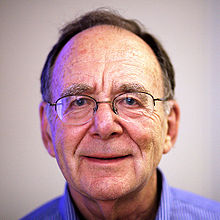
\includegraphics[width=1.0\textwidth]{Karp.jpg}%
     \end{minipage}%
   \end{center}
 \end{figure}
} 

\frame{
	\frametitle{ {\sc Hopcroft-Karp} algorithm [1973] }

		\begin{algorithmic}[1]
\STATE $\mathbf{M= \{\}}$; //set initial matching as empty set;
\WHILE{  \texttt{TRUE} }
\STATE find  the \textcolor{red}{\bf maximal shortest augmenting paths} $P = \{P_1, P_2, ..., P_k \}$  w.r.t. to $M$; 
\IF { no augmenting path was found }
\STATE break;
\ENDIF
\STATE augment $M$ using $P$ by $M = M \oplus P_1 \oplus P_2 \oplus ... \oplus P_k$; 
\ENDWHILE
\RETURN $\mathbf{M}$;
\end{algorithmic}

\begin{itemize}
\item 
Time complexity: $O(m \sqrt{n} )$. 
\item Key point: instead of considering each augmenting path individually, the algorithm consider the entire phase as \textcolor{red}{\bf blocking flow} in the {\sc Dinic's} algorithm. 
\end{itemize}

}




\frame{
	\frametitle{Property of consecutive augmentations} 
\begin{theorem}
 Let $M_0$ be a matching, $P_0$ a shortest augmenting path w.r.t. $M_0$, and $P_1$ an augmenting path w.r.t. $M_1=M_0\oplus P_0$. Then 
 $|P_1|  \geq |P_0| + |P_0\cap P_1|$.
\end{theorem}

\begin{figure}
\begin{tikzpicture}[scale=0.8, auto,swap]

    % Draw a 7,11 network
    % First we draw the vertices
    \def\dx{-12}; 
%    \foreach \pos/\name/\label in {{(0+\dx,0)/I1/I_1}, {(0+\dx,-1)/I2/I_2}, {(0+\dx,-2)/I3/I_3}, {(0+\dx,-3)/I4/I_4},{(0+\dx,-4)/I5/I_5},{(2+\dx, 0)/J1/J_1}, {(2+\dx, -1)/J2/J_2}, {(2+\dx, -2)/J3/J_3},{(2+\dx, -3)/J4/J_4},{(2+\dx, -4)/J5/J_5}}    
    \foreach \pos/\name/\label in {{(0+\dx,0)/I1/I_1}, {(0+\dx,-1)/I2/I_2}, {(0+\dx,-2)/I3/I_3}, {(0+\dx,-3)/I4/I_4},{(2+\dx, 0)/J1/J_1}, {(2+\dx, -1)/J2/J_2}, {(2+\dx, -2)/J3/J_3},{(2+\dx, -3)/J4/J_4}}
        \node[middlesmallvertex,draw=black, fill=blue!20] (\name) at \pos {\tiny $\label$};
  
    % Connect vertices with edges and draw weights
  \foreach \source/ \dest /\weight in {I1/J1/{}, I1/J2/{}, I1/J3/{}, I1/J4/{}, I2/J1/{}, I2/J4/{}, I3/J1/{}, I3/J4/{}, I4/J1/{}, I4/J2/{}, I4/J3/{}, I4/J4/{}}
          \path[undirectededge] (\source) -- node[weight] {$\weight$} (\dest);

  \foreach \source/ \dest /\weight in {I1/J1/{}}
          \path[undirectededge, red, ultra thick] (\source) -- node[weight] {$\weight$} (\dest);

%       \draw[dashed, ->] (0,0) arc  (120:60:2);
\node[ultra thick] at (1+\dx, -4) {$M_0$}; 


    \def\dx{-9}; 
    \foreach \pos/\name/\label in { {(0+\dx,-3)/I4/I_4}, {(2+\dx, -3)/J4/J_4}}
        \node[middlesmallvertex,draw=black, fill=blue!20] (\name) at \pos {\tiny $\label$};
  
  \foreach \source/ \dest /\weight in {I4/J4/{}}
          \path[undirectededge] (\source) -- node[weight] {$\weight$} (\dest);

  \foreach \source/ \dest /\weight in { I4/J4/{}}
          \path[undirectededge, red, ultra thick] (\source) -- node[weight] {$\weight$} (\dest);

\node[ultra thick] at (1+\dx, -4) {$P_0$}; 


    % Draw a 7,11 network
    % First we draw the vertices
    \def\dx{-6}; 
    \foreach \pos/\name/\label in {{(0+\dx,0)/I1/I_1}, {(0+\dx,-1)/I2/I_2}, {(0+\dx,-2)/I3/I_3}, {(0+\dx,-3)/I4/I_4},{(2+\dx, 0)/J1/J_1}, {(2+\dx, -1)/J2/J_2}, {(2+\dx, -2)/J3/J_3},{(2+\dx, -3)/J4/J_4}}
        \node[middlesmallvertex,draw=black, fill=blue!20] (\name) at \pos {\tiny $\label$};
  
    % Connect vertices with edges and draw weights
  \foreach \source/ \dest /\weight in {I1/J1/{}, I1/J2/{}, I1/J3/{}, I1/J4/{}, I2/J1/{}, I2/J4/{}, I3/J1/{}, I3/J4/{}, I4/J1/{}, I4/J2/{}, I4/J3/{}, I4/J4/{}}
          \path[undirectededge] (\source) -- node[weight] {$\weight$} (\dest);
  \foreach \source/ \dest /\weight in {I1/J1/{}, I4/J4/{}}
          \path[undirectededge, red, ultra thick] (\source) -- node[weight] {$\weight$} (\dest);
%       \draw[dashed, ->] (0,0) arc  (120:60:2);
\node[ultra thick] at (1+\dx, -4) {$M_1$}; 

    \def\dx{-3}; 
    \foreach \pos/\name/\label in {   {(0+\dx,-2)/I3/I_3}, {(0+\dx,-3)/I4/I_4},  {(2+\dx, -2)/J3/J_3},{(2+\dx, -3)/J4/J_4}}
        \node[middlesmallvertex,draw=black, fill=blue!20] (\name) at \pos {\tiny $\label$};
  
  \foreach \source/ \dest /\weight in {I4/J4/{}, I3/J4/{}, I4/J3/{}}
          \path[undirectededge] (\source) -- node[weight] {$\weight$} (\dest);

  \foreach \source/ \dest /\weight in { I4/J4/{}}
          \path[undirectededge, red, ultra thick] (\source) -- node[weight] {$\weight$} (\dest);

\node[ultra thick] at (1+\dx, -4) {$P_1$}; 




    % Draw a 7,11 network
    % First we draw the vertices
    \def\dx{0}; 
    \foreach \pos/\name/\label in {{(0+\dx,0)/I1/I_1}, {(0+\dx,-1)/I2/I_2}, {(0+\dx,-2)/I3/I_3}, {(0+\dx,-3)/I4/I_4},{(2+\dx, 0)/J1/J_1}, {(2+\dx, -1)/J2/J_2}, {(2+\dx, -2)/J3/J_3},{(2+\dx, -3)/J4/J_4}}
        \node[middlesmallvertex,draw=black, fill=blue!20] (\name) at \pos {\tiny $\label$};
  
    % Connect vertices with edges and draw weights
  \foreach \source/ \dest /\weight in {I1/J1/{}, I1/J2/{}, I1/J3/{}, I1/J4/{}, I2/J1/{}, I2/J4/{}, I3/J1/{}, I3/J4/{}, I4/J1/{}, I4/J2/{}, I4/J3/{}, I4/J4/{}}
          \path[undirectededge] (\source) -- node[weight] {$\weight$} (\dest);
  \foreach \source / \dest /\weight in {I1/J1/{},  I3/J4/{},  I4/J3/{}}
          \path[undirectededge, red, ultra thick] (\source) -- node[weight] {$\weight$} (\dest);
%       \draw[dashed, ->] (0,0) arc  (120:60:2);
 \node[ultra thick] at (1+\dx, -4) {$ M_2$}; 

   \end{tikzpicture}
\end{figure}

For example, $|P_0|=1$, $|P_1|=3$, and $|P_0\cap P_1|$ = 1. 
	
} 

\frame{

\begin{figure}
\begin{tikzpicture}[scale=0.8, auto,swap]

    % Draw a 7,11 network
    % First we draw the vertices
    \def\dx{-6}; 
    \foreach \pos/\name/\label in {{(0+\dx,0)/I1/I_1}, {(0+\dx,-1)/I2/I_2}, {(0+\dx,-2)/I3/I_3}, {(0+\dx,-3)/I4/I_4},{(2+\dx, 0)/J1/J_1}, {(2+\dx, -1)/J2/J_2}, {(2+\dx, -2)/J3/J_3},{(2+\dx, -3)/J4/J_4}}
        \node[middlesmallvertex,draw=black, fill=blue!20] (\name) at \pos {\tiny $\label$};
  
    % Connect vertices with edges and draw weights
%  \foreach \source/ \dest /\weight in {I1/J1/{}, I1/J3/{},  I2/J1/{}, I2/J3/{}, I3/J1/{}, I3/J2/{}, I3/J3/{}, I3/J4/{}, I4/J3/{}, I4/J4/{}}
%          \path[undirectededge] (\source) -- node[weight] {$\weight$} (\dest);
  \foreach \source/ \dest /\weight in {I3/J4/{}, I4/J3/{}}
          \path[undirectededge, red, ultra thick] (\source) -- node[weight] {$\weight$} (\dest);
%       \draw[dashed, ->] (0,0) arc  (120:60:2);
 \node[ultra thick] at (1+\dx, -4) {$ M_0\oplus M_2$}; 


 
    % Draw a 7,11 network
    % First we draw the vertices
    \def\dx{0}; 
    \foreach \pos/\name/\label in { {(0+\dx,-2)/I3/I_3}, {(0+\dx,-3)/I4/I_4},  {(2+\dx, -2)/J3/J_3},{(2+\dx, -3)/J4/J_4}}
        \node[middlesmallvertex,draw=black, fill=blue!20] (\name) at \pos {\tiny $\label$};
  
    % Connect vertices with edges and draw weights
  \foreach \source/ \dest /\weight in {I4/J3/{}, I3/J4/{}}
          \path[undirectededge] (\source) -- node[weight] {$\weight$} (\dest);
%  \foreach \source/ \dest /\weight in {I1/J1/{}, I2/J3/{},  I3/J2/{},  I4/J4/{}}
%          \path[undirectededge, red, ultra thick] (\source) -- node[weight] {$\weight$} (\dest);
%       \draw[dashed, ->] (0,0) arc  (120:60:2);
 \node[ultra thick] at (1+\dx, -4) {$ P_0\oplus P_1$}; 

   \end{tikzpicture}
\end{figure}


\begin{proof}
	\begin{itemize}
		\item Let's consider $P_0 \oplus P_1$.  We have the following two properties: 
			\begin{itemize}
				\item $ P_0 \oplus P_1 = M_0\oplus M_2$.
				\item Since $|M_2| = |M_0| + 2$,   $M_0\oplus M_2$ contains at least 2 vertex-disjoint augmenting paths w.r.t. $M_0$; call them $p$ and $p'$. We have $|p| \geq |P_0|$, and $|p'| \geq |P_0|$, as $P_0$ is the shortest one.
			\end{itemize}
		\item  Thus, $|P_0 \oplus P_1| = |M_0\oplus M_2| \geq |p| + |p'| \geq 2 |P_0| $.
		\item  Since $|P_0 \oplus P_1| = |P_0| + |P_1| - |P_0\cap P_1|$, we have $|P_1| \geq |P_0| + |P_1\cap P_0|$.  
	\end{itemize}
\end{proof}
}

\frame{
	\frametitle{Property of consecutive augmentations   (cont'd) } 

\begin{theorem}
	Starting with a matching $M_0$, compute a sequence $\textcolor{red}{\bf M_0}, \textcolor{blue}{\bf P_0}, \textcolor{red}{\bf M_1}, \textcolor{blue}{\bf P_1}, \textcolor{red}{\bf M_2}, \textcolor{blue}{\bf P_2},....$, where $P_i$ represents a \textcolor{blue}{\bf shortest augmenting path} w.r.t. $M_i$, and $M_{i+1} = M_i \oplus P_i$. We have $|P_{j} |\geq |P_i|$ (for $j > i$). If $|P_{j} | =  |P_i|$, $P_{j}$ and $P_i$ should be \textcolor{red}{\bf vertex-disjoint}, and thus both of them are augmenting paths w.r.t. $M_0$.  				
\end{theorem}

\begin{figure}
\begin{tikzpicture}[scale=0.8, auto,swap]

    % Draw a 7,11 network
    % First we draw the vertices
    \def\dx{-12}; 
    \foreach \pos/\name/\label in {{(0+\dx,0)/I1/I_1}, {(0+\dx,-1)/I2/I_2}, {(0+\dx,-2)/I3/I_3}, {(0+\dx,-3)/I4/I_4},{(2+\dx, 0)/J1/J_1}, {(2+\dx, -1)/J2/J_2}, {(2+\dx, -2)/J3/J_3},{(2+\dx, -3)/J4/J_4}}
        \node[middlesmallvertex,draw=black, fill=blue!20] (\name) at \pos {\tiny $\label$};
  
    % Connect vertices with edges and draw weights
  \foreach \source/ \dest /\weight in {I1/J1/{}, I1/J2/{}, I1/J3/{}, I1/J4/{}, I2/J1/{}, I2/J4/{}, I3/J1/{}, I3/J4/{}, I4/J1/{}, I4/J2/{}, I4/J3/{}, I4/J4/{}}
          \path[undirectededge] (\source) -- node[weight] {$\weight$} (\dest);
  \foreach \source/ \dest /\weight in {I1/J1/{}, I4/J4/{}}
          \path[undirectededge, red, ultra thick] (\source) -- node[weight] {$\weight$} (\dest);
%       \draw[dashed, ->] (0,0) arc  (120:60:2);
\node[ultra thick] at (1+\dx, -4) {$M_0$}; 

    \def\dx{-9}; 
    \foreach \pos/\name/\label in {   {(0+\dx,-2)/I3/I_3}, {(0+\dx,-3)/I4/I_4},  {(2+\dx, -2)/J3/J_3},{(2+\dx, -3)/J4/J_4}}
        \node[middlesmallvertex,draw=black, fill=blue!20] (\name) at \pos {\tiny $\label$};
  
  \foreach \source/ \dest /\weight in {I4/J4/{}, I3/J4/{}, I4/J3/{}}
          \path[undirectededge] (\source) -- node[weight] {$\weight$} (\dest);

  \foreach \source/ \dest /\weight in { I4/J4/{}}
          \path[undirectededge, red, ultra thick] (\source) -- node[weight] {$\weight$} (\dest);

\node[ultra thick] at (1+\dx, -4) {$P_0$}; 




    % Draw a 7,11 network
    % First we draw the vertices
    \def\dx{-6}; 
    \foreach \pos/\name/\label in {{(0+\dx,0)/I1/I_1}, {(0+\dx,-1)/I2/I_2}, {(0+\dx,-2)/I3/I_3}, {(0+\dx,-3)/I4/I_4},{(2+\dx, 0)/J1/J_1}, {(2+\dx, -1)/J2/J_2}, {(2+\dx, -2)/J3/J_3},{(2+\dx, -3)/J4/J_4}}
        \node[middlesmallvertex,draw=black, fill=blue!20] (\name) at \pos {\tiny $\label$};
  
    % Connect vertices with edges and draw weights
  \foreach \source/ \dest /\weight in {I1/J1/{}, I1/J2/{}, I1/J3/{}, I1/J4/{}, I2/J1/{}, I2/J4/{}, I3/J1/{}, I3/J4/{}, I4/J1/{}, I4/J2/{}, I4/J3/{}, I4/J4/{}}
          \path[undirectededge] (\source) -- node[weight] {$\weight$} (\dest);
  \foreach \source / \dest /\weight in {I1/J1/{},  I3/J4/{},  I4/J3/{}}
          \path[undirectededge, red, ultra thick] (\source) -- node[weight] {$\weight$} (\dest);
%       \draw[dashed, ->] (0,0) arc  (120:60:2);
 \node[ultra thick] at (1+\dx, -4) {$ M_1$}; 

    \def\dx{-3}; 
    \foreach \pos/\name/\label in {{(0+\dx,0)/I1/I_1}, {(0+\dx,-1)/I2/I_2},  {(2+\dx, 0)/J1/J_1}, {(2+\dx, -1)/J2/J_2}}
        \node[middlesmallvertex,draw=black, fill=blue!20] (\name) at \pos {\tiny $\label$};
  
  \foreach \source/ \dest /\weight in {I1/J2/{}, I2/J1/{}, I1/J1/{}}
          \path[undirectededge] (\source) -- node[weight] {$\weight$} (\dest);

  \foreach \source/ \dest /\weight in { I1/J1/{}}
          \path[undirectededge, red, ultra thick] (\source) -- node[weight] {$\weight$} (\dest);

\node[ultra thick] at (1+\dx, -4) {$P_1$}; 


%
%    % Draw a 7,11 network
%    % First we draw the vertices
%    \def\dx{0}; 
%    \foreach \pos/\name/\label in {{(0+\dx,0)/I1/I_1}, {(0+\dx,-1)/I2/I_2}, {(0+\dx,-2)/I3/I_3}, {(0+\dx,-3)/I4/I_4},{(2+\dx, 0)/J1/J_1}, {(2+\dx, -1)/J2/J_2}, {(2+\dx, -2)/J3/J_3},{(2+\dx, -3)/J4/J_4}}
%        \node[middlesmallvertex,draw=black, fill=blue!20] (\name) at \pos {\tiny $\label$};
%  
%    % Connect vertices with edges and draw weights
%  \foreach \source/ \dest /\weight in {I1/J1/{}, I1/J2/{}, I1/J3/{}, I1/J4/{}, I2/J1/{}, I2/J4/{}, I3/J1/{}, I3/J4/{}, I4/J1/{}, I4/J2/{}, I4/J3/{}, I4/J4/{}}
%          \path[undirectededge] (\source) -- node[weight] {$\weight$} (\dest);
%  \foreach \source / \dest /\weight in {I1/J1/{},  I3/J4/{},  I4/J3/{}}
%          \path[undirectededge, red, ultra thick] (\source) -- node[weight] {$\weight$} (\dest);
%%       \draw[dashed, ->] (0,0) arc  (120:60:2);
% \node[ultra thick] at (1+\dx, -4) {$ M_2$}; 


   \end{tikzpicture}
\end{figure}
	
}

\frame{
%	\frametitle{Proof}
	\begin{proof}
		\begin{itemize}
			\item Suppose, for contradiction, that $|P_j| = |P_i|$ (for $j > i$), but $P_j$ and $P_i$ are not vertex-disjoint. 
			\item Then there exist $k$ and $l$ such that $i \leq k < l \leq j$, $P_k$ and $P_l$ are not vertex-disjoint, and for each $m$, $k < m < l$, $P_m$ is vertex-disjoint from $P_k$ and $P_l$. 
			\item Then $P_l$ is an augmenting path w.r.t. $M_k\oplus P_k$. 
			\item So $|P_l| \geq |P_k| + |P_k\cap P_l|$. 
			\item But $|P_l| = |P_k|$, so $|P_l \cap P_k| = 0$, i.e., $P_l$ and $P_k$ has no common edge. If $P_l$ and $P_k$ has a common vertex $v$, they should have in common that edge incident with $v$ which is in $M_k\oplus P_k$. A contradiction.  
		\end{itemize}
	\end{proof}
 
 \begin{figure}
\begin{tikzpicture}[scale=0.8, auto,swap]

    \foreach \pos/\name/\label in {{(0,1)/I1/I_1}, {(0,-1)/I2/I_2},{(1,0)/I3/I_3},{(2,0)/I4/I_4},{(3,1)/I5/I_5},{(3,-1)/I6/I_6}}
        \node[middlesmallvertex,draw=black, fill=blue!20] (\name) at \pos {\tiny $\label$};
  
    % Connect vertices with edges and draw weights
  \foreach \source/ \dest /\weight in {I1/I3/{}, I2/I3/{}, I3/I4/{}, I4/I5/{}, I4/I6/{}}
          \path[undirectededge] (\source) -- node[weight] {$\weight$} (\dest);

  \foreach \source/ \dest /\weight in {I3/I4/{}}
          \path[undirectededge, red, ultra thick] (\source) -- node[weight] {$\weight$} (\dest);

\node[ultra thick] at (1.5, 1) {$P_l$}; 

\node[ultra thick] at (1.5, -0.8) {$M_k\oplus P_k$}; 

    \end{tikzpicture}
\end{figure}
	
}

\frame{
	\frametitle{Time complexity of the  {\sc Hopcroft-Karp} algorithm} 
	\begin{theorem}
	Let $s$ be the cardinality of the maximum matching. The  \textcolor{red}{\bf number of distinct path lengths}  $|P_0|, |P_1|, |P_2|,..., |P_{s-1}| $ is less than or equal to $2\lfloor\sqrt{s}\rfloor + 2$.
	\end{theorem}
\begin{proof}
	\begin{itemize}
			\item Let's divide these augmenting steps into two parts: 
			\begin{itemize} 
				\item The first $r=\lfloor s - \sqrt{s} \rfloor$ steps:  after $r$ steps, the matching has size $|M_r| = r$; however, the path length increases to at most $2\sqrt{s}+1$, since $|P_r| \leq 2\lfloor\frac{s-\sqrt{s}}{\sqrt{s}}\rfloor +1 \leq 2\lfloor\sqrt{s}\rfloor + 1$. 	 (Reason:  For any $r$, we have $ | P_r | \leq 2 \lfloor\frac{r}{s-r}\rfloor$, since $M_s \oplus M_r$ contains at least $s-r$ vertex-disjoint (and hence edge-disjoint) augmenting paths w.r.t. $M_r$. Altogether these paths contains at most $r$ edges from $M_r$. So one of them must have less than $\lfloor\frac{r}{s-r}\rfloor$ edges from $M_r$.) 
				\item The others $\sqrt{s}$ steps: each step increases path length at most $1$. 
			\end{itemize}	
	\end{itemize}
\end{proof}
}

\frame{
	\frametitle{Time complexity of the  {\sc Hopcroft-Karp} algorithm} 
\begin{itemize}
	\item The fact of at most $2\sqrt{s} + 1$ distinct numbers in path length sequence implies that the path sequence can be divided into at most $2\sqrt{s} + 1$ phases, each phase containing shortest augmenting paths with identical length. 
	\item The following properties are immediate: the paths in a phase are vertex-disjoint, and they are augmenting paths w.r.t. the matching from which this phase begun.  
	\item Thus, we should not regard successive augmenting steps are independent, but should concentrate on efficient implementation of \textcolor{red}{\bf the entire phase}, i.e., finding \textcolor{red}{\bf the maximal collection of augmenting shortest paths}. 
	\item Note that this analysis works for general graphs. 
	\item For bipartite graphs,  \textcolor{red}{\bf the maximal collection of augmenting shortest paths}, forming \textcolor{red}{\bf $M$-alternating forest}, can be found using BFS and DFS technique in $O(m)$ time, as \textcolor{red}{\bf layered network} identified in {\sc Dinic's} algorithm. 
	\item Thus the total cost is $O(m \sqrt{n})$ for bipartite graphs as each phase cost $O(m)$ time. 
\end{itemize}
} 	

\frame{
	\frametitle{ {\sc Hopcroft-Karp} algorithm: a detailed version }

		\begin{algorithmic}[1]
\STATE $\mathbf{M= \{\}}$; //set initial matching as empty set;
\WHILE{  \texttt{TRUE} }
\STATE Constructing  a \textcolor{red}{\bf layered network} by running BFS over graph $G$, where the edges in $M$ have direction from jobs to individuals, while edges in $E-M$ have reverse direction (Note: augmenting paths become directed path in $G$); 
\STATE Finding the \textcolor{red}{\bf maximal shortest augmenting paths}  $P = \{P_1, P_2, ..., P_k \}$  w.r.t. to $M$ by running DFS guided by the layer network;  (removing a path as soon as it was identified to guarantee them to be vertex-disjoint)
\IF { no augmenting path was found }
\STATE break;
\ENDIF
\STATE Augmenting $M$ using $P$ by $M = M \oplus P_1 \oplus P_2 \oplus ... \oplus P_k$; 
\ENDWHILE
\RETURN $\mathbf{M}$;
\end{algorithmic}

Time complexity: $O(m \sqrt{n} )$. 
 
}

\frame{
	\frametitle{An example: finding $P_2$ and $P_3$ in phase 2 }


\begin{figure}
\begin{tikzpicture}[scale=0.75, auto,swap]

    % Draw a 7,11 network
    % First we draw the vertices
    \def\dx{-12}; 
    \foreach \pos/\name/\label in {{(0+\dx,0)/I1/I_1}, {(0+\dx,-1)/I2/I_2}, {(0+\dx,-2)/I3/I_3}, {(0+\dx,-3)/I4/I_4},{(2+\dx, 0)/J1/J_1}, {(2+\dx, -1)/J2/J_2}, {(2+\dx, -2)/J3/J_3},{(2+\dx, -3)/J4/J_4}}
        \node[middlesmallvertex,draw=black, fill=blue!20] (\name) at \pos {\tiny $\label$};
  
    % Connect vertices with edges and draw weights
  \foreach \source/ \dest /\weight in {I1/J1/{}, I1/J2/{}, I1/J3/{}, I1/J4/{}, I2/J1/{}, I2/J4/{}, I3/J1/{}, I3/J4/{}, I4/J1/{}, I4/J2/{}, I4/J3/{}, I4/J4/{}}
          \path[undirectededge] (\source) -- node[weight] {$\weight$} (\dest);
  \foreach \source/ \dest /\weight in {I1/J1/{}, I4/J4/{}}
          \path[undirectededge, red, ultra thick] (\source) -- node[weight] {$\weight$} (\dest);
%       \draw[dashed, ->] (0,0) arc  (120:60:2);
\node[ultra thick] at (1+\dx, -3.6) {$M_2$}; 

    \def\dx{-9}; 
    \foreach \pos/\name/\label in {   {(0+\dx,-2)/I3/I_3}, {(0+\dx,-3)/I4/I_4},  {(2+\dx, -2)/J3/J_3},{(2+\dx, -3)/J4/J_4}}
        \node[middlesmallvertex,draw=black, fill=blue!20] (\name) at \pos {\tiny $\label$};
  
  \foreach \source/ \dest /\weight in {I4/J4/{}, I3/J4/{}, I4/J3/{}}
          \path[undirectededge] (\source) -- node[weight] {$\weight$} (\dest);

  \foreach \source/ \dest /\weight in { I4/J4/{}}
          \path[undirectededge, red, ultra thick] (\source) -- node[weight] {$\weight$} (\dest);

\node[ultra thick] at (1+\dx, -3.6) {$P_2$}; 




    % Draw a 7,11 network
    % First we draw the vertices
    \def\dx{-6}; 
    \foreach \pos/\name/\label in {{(0+\dx,0)/I1/I_1}, {(0+\dx,-1)/I2/I_2}, {(0+\dx,-2)/I3/I_3}, {(0+\dx,-3)/I4/I_4},{(2+\dx, 0)/J1/J_1}, {(2+\dx, -1)/J2/J_2}, {(2+\dx, -2)/J3/J_3},{(2+\dx, -3)/J4/J_4}}
        \node[middlesmallvertex,draw=black, fill=blue!20] (\name) at \pos {\tiny $\label$};
  
    % Connect vertices with edges and draw weights
  \foreach \source/ \dest /\weight in {I1/J1/{}, I1/J2/{}, I1/J3/{}, I1/J4/{}, I2/J1/{}, I2/J4/{}, I3/J1/{}, I3/J4/{}, I4/J1/{}, I4/J2/{}, I4/J3/{}, I4/J4/{}}
          \path[undirectededge] (\source) -- node[weight] {$\weight$} (\dest);
  \foreach \source / \dest /\weight in {I1/J1/{},  I3/J4/{},  I4/J3/{}}
          \path[undirectededge, red, ultra thick] (\source) -- node[weight] {$\weight$} (\dest);
%       \draw[dashed, ->] (0,0) arc  (120:60:2);
 \node[ultra thick] at (1+\dx, -3.6) {$ M_3$}; 

    \def\dx{-3}; 
    \foreach \pos/\name/\label in {{(0+\dx,0)/I1/I_1}, {(0+\dx,-1)/I2/I_2},  {(2+\dx, 0)/J1/J_1}, {(2+\dx, -1)/J2/J_2}}
        \node[middlesmallvertex,draw=black, fill=blue!20] (\name) at \pos {\tiny $\label$};
  
  \foreach \source/ \dest /\weight in {I1/J2/{}, I2/J1/{}, I1/J1/{}}
          \path[undirectededge] (\source) -- node[weight] {$\weight$} (\dest);

  \foreach \source/ \dest /\weight in { I1/J1/{}}
          \path[undirectededge, red, ultra thick] (\source) -- node[weight] {$\weight$} (\dest);

\node[ultra thick] at (1+\dx, -3.6) {$P_3$}; 


%
%    % Draw a 7,11 network
%    % First we draw the vertices
%    \def\dx{0}; 
%    \foreach \pos/\name/\label in {{(0+\dx,0)/I1/I_1}, {(0+\dx,-1)/I2/I_2}, {(0+\dx,-2)/I3/I_3}, {(0+\dx,-3)/I4/I_4},{(2+\dx, 0)/J1/J_1}, {(2+\dx, -1)/J2/J_2}, {(2+\dx, -2)/J3/J_3},{(2+\dx, -3)/J4/J_4}}
%        \node[middlesmallvertex,draw=black, fill=blue!20] (\name) at \pos {\tiny $\label$};
%  
%    % Connect vertices with edges and draw weights
%  \foreach \source/ \dest /\weight in {I1/J1/{}, I1/J2/{}, I1/J3/{}, I1/J4/{}, I2/J1/{}, I2/J4/{}, I3/J1/{}, I3/J4/{}, I4/J1/{}, I4/J2/{}, I4/J3/{}, I4/J4/{}}
%          \path[undirectededge] (\source) -- node[weight] {$\weight$} (\dest);
%  \foreach \source / \dest /\weight in {I1/J1/{},  I3/J4/{},  I4/J3/{}}
%          \path[undirectededge, red, ultra thick] (\source) -- node[weight] {$\weight$} (\dest);
%%       \draw[dashed, ->] (0,0) arc  (120:60:2);
% \node[ultra thick] at (1+\dx, -4) {$ M_2$}; 

%Graph G

    \def\dx{-12}; 
    \def\dy{-4.5}; 
    
    \foreach \pos/\name/\label in {{(0+\dx,0+\dy)/I1/I_1}, {(0+\dx,-1+\dy)/I2/I_2}, {(0+\dx,-2+\dy)/I3/I_3}, {(0+\dx,-3+\dy)/I4/I_4},{(2+\dx, 0+\dy)/J1/J_1}, {(2+\dx, -1+\dy)/J2/J_2}, {(2+\dx, -2+\dy)/J3/J_3},{(2+\dx, -3+\dy)/J4/J_4}}
        \node[middlesmallvertex,draw=black, fill=blue!20] (\name) at \pos {\tiny $\label$};

    \foreach \pos/\name/\label in {{(-1.5+\dx,-1.5+\dy)/s/s}, {(3.5+\dx,-1.5+\dy)/t/t}}
        \node[middlesmallvertex,draw=black, fill=green!20] (\name) at \pos {\tiny $\label$};
          
    % Connect vertices with edges and draw weights
  \foreach \source/ \dest /\weight in { I1/J2/{}, I1/J3/{}, I1/J4/{}, I2/J1/{}, I2/J4/{}, I3/J1/{}, I3/J4/{}, I4/J1/{}, I4/J2/{}, I4/J3/{}, I1/s/{}, s/I2/{}, s/I3/{}, I4/s/{}, t/J1/{},J2/t/{},J3/t/{},t/J4/{}}
          \draw[->, thick] (\source) -- node[weight] {$\weight$} (\dest);
  \foreach \source/ \dest /\weight in {J1/I1/{}, J4/I4/{}}
          \draw[->, red, ultra thick] (\source) -- node[weight] {$\weight$} (\dest);
%       \draw[dashed, ->] (0,0) arc  (120:60:2);
\node[ultra thick] at (1+\dx, -3.6+\dy) {$G$}; 

%layered network 
    \def\dx{-7.5}; 
    \def\dy{-6}; 
    
    \foreach \pos/\name/\label in {{(1+\dx,1+\dy)/I2/I_2}, {(1+\dx,-1+\dy)/I3/I_3}, {(3+\dx,1+\dy)/J1/J_1}, {(3+\dx,-1+\dy)/J4/J_4},{(5+\dx, 1+\dy)/I1/I_1}, {(5+\dx, -1+\dy)/I4/I_4}, {(7+\dx, 1+\dy)/J3/J_3},{(7+\dx, -1+\dy)/J2/J_2}}
        \node[middlesmallvertex,draw=black, fill=blue!20] (\name) at \pos {\tiny $\label$};
 
     \foreach \pos/\name/\label in {{(0+\dx,0+\dy)/s/s}, {(8+\dx,0+\dy)/t/t}}
        \node[middlesmallvertex,draw=black, fill=green!20] (\name) at \pos {\tiny $\label$};
  
    % Connect vertices with edges and draw weights
  \foreach \source/ \dest /\weight in { I2/J1/{}, I2/J4/{}, I3/J1/{}, I3/J4/{}, I4/J3/{},  I4/J2/{}, I1/J3/{}, I1/J2/{}, s/I2/{}, s/I3/{}, J2/t/{},J3/t/{} }
          \draw[->, thick] (\source) -- node[weight] {$\weight$} (\dest);
  \foreach \source/ \dest /\weight in {J1/I1/{}, J4/I4/{}}
          \draw[->, red, ultra thick] (\source) -- node[weight] {$\weight$} (\dest);
%       \draw[dashed, ->] (0,0) arc  (120:60:2);
\node[ultra thick] at (4+\dx, -1.7+\dy) {Layered network and shortest $s-t$ paths}; 

   \end{tikzpicture}
\end{figure}
Note: the shortest augmenting paths w.r.t. $M_2$ are in one-to-one correspondence with the shortest $s-t$ paths in $G$.  
}

%\frame{
%	\frametitle{Time complexity analysis}
%		\begin{theorem}
%			The {\sc Hopcroft-Karp} algorithm runs in $O(m \sqrt{n} )$. 
%		\end{theorem}
%		\begin{proof}
%			\begin{itemize}
%				\item As done in the Dinic's algorithm, the execution of the {\sc Hopcroft-Karp} algorithm is divided into phases. 
%				\item The first $\sqrt{n}$ phases cost $O(m \sqrt{n} )$ time by running BFS and DFS search on the residual graph. 
%				\item Note that each phase increases the length of the shortest path by at least one (why?). 
%				\item After the first $\sqrt{n}$ phases, the augmenting path should be at least $\sqrt{n}$ long. 
%				\item Now let consider the difference between the maximum matching $M^*$ and the improved $M$ is at most $\sqrt{n}$.should be at most $\sqrt{n}$ paths. 
%				\item Therefore the difference between the maximum matching $M^*$ and the improved $M$ is at most $\sqrt{n}$. 
%				\item Thus, at most $\sqrt{n}$ phases are needed. 
%			\end{itemize}
%		\end{proof}
%}

\frame{
	\begin{block}{}
		1.4 ILP formulation and its dual problem
	\end{block}
} 

\frame{
	\frametitle{ILP formulation for maximum-matching problem} 

\begin{figure}
    \begin{tikzpicture}[scale=1., auto,swap]
    % Draw a 7,11 network
    % First we draw the vertices
    \node at (0, 0.5) {$I$};
    \node at (2, 0.5) {$J$};
    
    \foreach \pos/\name/\label in {{(0,0)/I1/I_1}, {(0,-1)/I2/I_2}, {(0,-2)/I3/I_3}, {(2, 0)/J1/J_1}, {(2, -1)/J2/J_2}, {(2, -2)/J3/J_3}}
        \node[middlesmallvertex,draw=black, fill=blue!20] (\name) at \pos {\tiny $\label$};
  
    % Connect vertices with edges and draw weights
   \foreach \source/ \dest /\weight in {I1/J2/{}, I2/J1/{}, I2/J2/{}, I2/J3/{}, I3/J2/{}, I3/J3/{}}
          \path[undirectededge] (\source) -- node[weight] {$\weight$} (\dest);
%       \draw[dashed, ->] (0,0) arc  (120:60:2);
   \end{tikzpicture}
\end{figure}					


\begin{small}
\[
\begin{array}{rrrrrrrrrrrr}
 \max & x_{12} &+ x_{21}&  +x_{22} & +x_{23} &  +x_{31}    &+x_{32}  & +x_{33}  & &  \\
s.t.     & x_{12}  &     &  & &  &   &&  \leq 1  & \text{node } I_1 \\
      &  & x_{21}  & +x_{22}  & +x_{23}   & & &  & \leq 1 & \text{node } I_2  \\
      & &  & &  &    & x_{32}  & +x_{33}  & \leq 1  & \text{node } I_3 \\
      & & x_{21}    &   & &  &  & & \leq 1   & \text{node } J_1\\
       & x_{12}  &  & +x_{22}  & &  & +x_{32} & & \leq 1 & \text{node } J_2  \\
      & &  & & x_{23} &    &  & +x_{33}  & \leq 1  & \text{node } J_3 \\
       &  &   &   &   & & &x_{ij} & = 0/1   & \\

\end{array} \nonumber
\]
\end{small}

}

\frame{
	\frametitle{Totally unimodular property } 
%\[
%\begin{array}{rrrrl}
% \max & \sum_{(i, j) \in E}  x_{ij}   & & & \\
% s.t. & \sum_{j=1}^n  x_{ij} & \leq & 1 & i=1, 2, ..., n\\
%       & \sum_{i=1}^n  x_{ij} & \leq & 1 & j=1, 2, ..., n\\
%       & x_{ij} & = & 0/1 & i, j=1, 2, ..., n\\
%\end{array} \nonumber
%\]
\begin{itemize}
	\item Note that the node-arc matrix is totally unimodular i.f.f. the graph is bipartite. 
	\item Thus, by relaxing the integrity constraint to $1 \geq x_{ij} \geq 0$, we have a linear program. Its dual problem is essentially the {\sc Vertex Cover}.  Here, $u_{i}$ denotes the dual variable for the individual $I_{i}$, while $v_{i}$ denotes the variable for the job $J_{i}$. 
\end{itemize}

\begin{small}
\[
\begin{array}{rrrrrrrrrrrr}
 \min & u_{{1}} &+ u_{{2}}&  + u_{{3}} & + v_{{1}} &  + v_{{2}}    & +v_{{3}}  &   & \\
s.t.  & u_{{1}} &    &   &  &  + v_{{2}}    &   &  \geq 1 & \text{edge } (I_1, J_2)\\
       &  & u_{{2}}&   & + v_{{1}} &    &   &  \geq 1 & \text{edge } (I_2, J_1)\\
       &  & u_{{2}}& & &  + v_{{2}}    &  &  \geq 1 & \text{edge } (I_2, J_2)\\
       &  & u_{{2}}&  &  &   & + v_{{3}}  &  \geq 1 & \text{edge } (I_2, J_3)\\
       &  & &   u_{{3}} &  &  + v_{{2}}    &  &  \geq 1 & \text{edge } (I_2, J_2)\\
       &  & u_{{2}}& & &    & +v_{{3}}  &  \geq 1 & \text{edge } (I_2, J_3)\\
       & u_{{1}} ,& u_{{2}},& u_{{3}}, & v_{{1}}, &  v_{{2}},    & v_{{3}}  &  \geq 0 & 
\end{array} \nonumber
\]
\end{small}

}

\frame{
	\frametitle{Dual problem:  {\sc MinVertexCover} } 
%\[
%\begin{array}{rrrrl}
% \max & \sum_{(i, j) \in E}  x_{ij}   & & & \\
% s.t. & \sum_{j=1}^n  x_{ij} & \leq & 1 & i=1, 2, ..., n\\
%       & \sum_{i=1}^n  x_{ij} & \leq & 1 & j=1, 2, ..., n\\
%       & x_{ij} & = & 0/1 & i, j=1, 2, ..., n\\
%\end{array} \nonumber
%\]
\begin{itemize}
	\item Note that the node-arc matrix is totally unimodular i.f.f. the graph is bipartite. 
	\item Thus, the dual problem is essentially the {\sc MinVertexCover} problem. 
\end{itemize}

\begin{small}
\[
\begin{array}{rrrrrrrrrrrr}
 \min & u_{{1}} &+ u_{{2}}&  + u_{{3}} & + v_{{1}} &  + v_{{2}}    & +v_{{3}}  &   & \\
s.t.  & u_{{1}} &    &   &  &  + v_{{2}}    &   &  \geq 1 & \text{edge } (I_1, J_2)\\
       &  & u_{{2}}&   & + v_{{1}} &    &   &  \geq 1 & \text{edge } (I_2, J_1)\\
       &  & u_{{2}}& & &  + v_{{2}}    &  &  \geq 1 & \text{edge } (I_2, J_2)\\
       &  & u_{{2}}&  &  &   & + v_{{3}}  &  \geq 1 & \text{edge } (I_2, J_3)\\
       &  & &   u_{{3}} &  &  + v_{{2}}    &  &  \geq 1 & \text{edge } (I_2, J_2)\\
       &  & u_{{2}}& & &    & +v_{{3}}  &  \geq 1 & \text{edge } (I_2, J_3)\\
       & u_{{1}} ,& u_{{2}},& u_{{3}}, & v_{{1}}, &  v_{{2}},    & v_{{3}}  &  = 0/1 & 
\end{array} \nonumber
\]
\end{small}

}
 
\frame{
	\begin{block}{}
		1.5 Konig's theorem: {\sc MaxMatching}  vs. {\sc MinVertexCover} 
	\end{block}
}

\frame{
\frametitle{ {\sc MinVertexCover } Problem }

\begin{itemize}
 \item 
Practical problem: \\ {\em 
Given n sites connected with paths, how many guards (or cameras)  should be deployed on sites to surveille {\bf all} the paths?}

\begin{block}{ {\sc MinVertexCover} problem}
 {\bf Input:} Given a graph $G=<V,E>$, \\
 {\bf Output:} Find the minimum set of nodes $S  \subseteq V$, such that each edge has at least one of its endpoints in $S$. 
\end{block}

%\item An example: are there 4 nodes to cover all edges in the following graph? 

\begin{figure}
\begin{tikzpicture}[scale=1.1, auto,swap]
    % Draw a 7,11 network
    % First we draw the vertices
    \foreach \pos/\name in {{(0,2)/v1}, {(2,2)/v2}, {(1,1)/v3}, {(2,1)/v4}, {(3,1)/v5}, {(0,0)/v6}, {(2,0)/v7}}
        \node[smallvertex, draw, fill=blue!20] (\name) at \pos {};
        
    % Connect vertices with edges and draw weights
    \foreach \source/ \dest /\weight in {v1/v2/{}, v1/v3/{}, v2/v3/{}, v2/v4/{}, v2/v5/{}, v3/v6/{}, v3/v7/{}, v6/v7/{}, v4/v7/{}, v5/v7/{}  }
        \path[undirectededge] (\source) -- node[weight] {$\weight$} (\dest);
%       \draw[dashed, ->] (0,0) arc  (120:60:2);

    \foreach \pos/\name in { {(2,2)/v2}, {(1,1)/v4}, {(2,0)/v7}}
        \node[smallvertex, draw, fill=yellow] (\name) at \pos {};


      \end{tikzpicture}

\end{figure}

\item In this example, the three nodes in yellow cover all edges. 
\end{itemize} 

} 

\frame{
	\frametitle{{\sc MaxMatching} vs. {\sc MinVertexCover}: Konig's theorem [1931]} 

\begin{itemize}
	\item Konig's theorem in terms of graph theory:
\end{itemize}
	
	\begin{theorem}
		For a bipartite graph $G$, the size of maximum matching equals  that of the minimum vertex cover. 
	\end{theorem}	
	
		


	\begin{figure}
    \begin{tikzpicture}[scale=0.65, auto,swap]
    % Draw a 7,11 network
    % First we draw the vertices
    \node at (0, 0.5) {$I$};
    \node at (2, 0.5) {$J$};
    
    \foreach \pos/\name/\label in {{(0,0)/I1/I_1}, {(0,-2)/I3/I_3}, {(2, 0)/J1/J_1}, {(2, -2)/J3/J_3}}
        \node[middlesmallvertex,draw=black, fill=blue!20] (\name) at \pos {\tiny $\label$};

    \foreach \pos/\name/\label in { {(0,-1)/I2/I_2}, {(2, -1)/J2/J_2}}
        \node[middlesmallvertex,draw=black, fill=yellow] (\name) at \pos {\tiny $\label$};
  
    % Connect vertices with edges and draw weights
   \foreach \source/ \dest /\weight in {I1/J2/{}, I2/J1/{},  I2/J3/{}, I3/J2/{}}
          \path[undirectededge] (\source) -- node[weight] {$\weight$} (\dest);
%       \draw[dashed, ->] (0,0) arc  (120:60:2);

   \foreach \source/ \dest /\weight in {I1/J2/{}, I2/J1/{}}
          \path[undirectededge, red, ultra thick] (\source) -- node[weight] {$\weight$} (\dest);

   \end{tikzpicture}
\end{figure}	
} 	

\frame{
\frametitle{{\sc MaxMatching} vs. {\sc MinVertexCover}: Konig's theorem [1931]} 

\begin{itemize}
	
\item Konig's theorem in the language of matrix:

\end{itemize}
	
	\begin{theorem}
		If the elements of a matrix are 0's and 1's, then the minimum number of rows and columns that will contains all of the 1's is equal to the maximum number of 1's that can be chosen, with no two in the same row or column. 
	\end{theorem}	


			
	
\begin{figure}
    \begin{tikzpicture}[scale=1., auto,swap]

          \path[undirectededge,  green] (-1, 0) --  (1, 0);
          \path[undirectededge,  green] (0, 0.7) --  (0, -0.7);

 
 \node at (0, 0) {$
\left[ \begin{array}{ccc}
0 & \textcolor{red}{1} & 0 \\
\textcolor{red}{1} & 0 & 1\\
0 & 1 & 0 
 \end{array} \right]
$}; 
 
   \end{tikzpicture}
\end{figure}	
	
}

\frame{
	\frametitle{ {\sc MaxMatching} vs. {\sc MinVertexCover}} 		

\begin{figure}
    \begin{tikzpicture}[scale=0.85, auto,swap]

    % Draw a 7,11 network
    % First we draw the vertices
    \node at (0, 0.5) {$I$};
    \node at (2, 0.5) {$J$};
    
    \foreach \pos/\name/\label in {{(0,0)/I1/I_1}, {(0,-2)/I3/I_3}, {(2, 0)/J1/J_1}, {(2, -2)/J3/J_3}}
        \node[middlesmallvertex,draw=black, fill=blue!20] (\name) at \pos {\tiny $\label$};

    \foreach \pos/\name/\label in { {(0,-1)/I2/I_2}, {(2, -1)/J2/J_2}}
        \node[middlesmallvertex,draw=black, fill=yellow] (\name) at \pos {\tiny $\label$};
  
    % Connect vertices with edges and draw weights
   \foreach \source/ \dest /\weight in {I1/J2/{}, I2/J1/{},  I2/J3/{}, I3/J2/{}}
          \path[undirectededge] (\source) -- node[weight] {$\weight$} (\dest);
%       \draw[dashed, ->] (0,0) arc  (120:60:2);

   \foreach \source/ \dest /\weight in {I1/J2/{}, I2/J1/{}}
          \path[undirectededge, red, ultra thick] (\source) -- node[weight] {$\weight$} (\dest);

   \end{tikzpicture}
\end{figure}				
\begin{itemize}
		\item Note that {\sc MinVertexCover} problem for general graphs is NP-Complete. However, when limited to bipartite graphs, {\sc MinVertexCover} problem is in $P$.  
		\item Actually, this theorem is a pre-linear programming example of duality. 
		%since   minimum vertex cover and maximum matching have identical size. 

	\item First, it is obvious that any vertex cover provides an upper bound for maximum matching (Reason: the edges in a matching share no common nodes; thus, to cover these edges, at least one of its ends should be selected.)
	\end{itemize}

	
}

\frame{
%	\frametitle{Konig's theorem [1931]}

		\begin{figure}
    \begin{tikzpicture}[scale=0.7, auto,swap]
    % Draw a 7,11 network
    % First we draw the vertices
    \node at (0, 0.5) {$I$};
    \node at (2, 0.5) {$J$};
    
       \node at (5, -1) {$F=\{I_{3}, J_{2}, I_{1}\}$};
       
    \foreach \pos/\name/\label in {{(0,0)/I1/I_1}, {(0,-2)/I3/I_3}, {(2, 0)/J1/J_1}, {(2, -2)/J3/J_3}}
        \node[middlesmallvertex,draw=black, fill=blue!20] (\name) at \pos {\tiny $\label$};

    \foreach \pos/\name/\label in { {(0,-1)/I2/I_2}, {(2, -1)/J2/J_2}}
        \node[middlesmallvertex,draw=black, fill=yellow] (\name) at \pos {\tiny $\label$};
  
    % Connect vertices with edges and draw weights
   \foreach \source/ \dest /\weight in {I1/J2/{}, I2/J1/{},  I2/J3/{}, I3/J2/{}}
          \path[undirectededge] (\source) -- node[weight] {$\weight$} (\dest);
%       \draw[dashed, ->] (0,0) arc  (120:60:2);

   \foreach \source/ \dest /\weight in {I1/J2/{}, I2/J1/{}}
          \path[undirectededge, red, ultra thick] (\source) -- node[weight] {$\weight$} (\dest);

   \end{tikzpicture}
\end{figure}	


	\begin{proof}
		\begin{itemize}
			\item Basic idea: For each edge in $M$, exactly one end will be selected.  We first divide the edges in $M$ into two categories:
	% $M=M_1\cup M_2$.
			\begin{enumerate}
				\item $M\cap F$: edges in \textcolor{red}{\bf an alternating tree rooted at an unmatched node in $I$}, say $(I_1,J_2)$. Here, $F$ denotes \textcolor{red}{\bf the forest} of this type of alternating trees. 
				\item $M-F$: the others edges, say $(I_2, J_1)$. 
			\end{enumerate} 
			\item Next, we select  $C=(I-F)\cup (J \cap F)$, i.e., \textcolor{red}{\bf right end} of edges in $M\cap F$, and \textcolor{red}{\bf left end} of edges in $M-F$.  
			\item $C$ forms a vertex cover since for any edge $(u,v)\notin M$, 
				\begin{itemize}
					\item If both $u$ and $v$ are matched, both of them will be selected. 
					\item				 	If $u$ is unmatched, then $(u, v) \in F$, and thus $v$ will be selected. 
					\item  If $v$ is unmatched,  then $u$ should be matched and thus be selected. 
			\end{itemize}
 
 		\end{itemize}             

	\end{proof}

	\begin{figure}
    \begin{tikzpicture}[scale=0.73, auto,swap]
    % Draw a 7,11 network
    % First we draw the vertices
    \node at (0, 0.5) {$I$};
    \node at (2, 0.5) {$J$};
    
    \foreach \pos/\name/\label in {{(0,0)/I1/I_1}, {(0,-2)/I3/I_3}, {(2, 0)/J1/J_1}, {(2, -2)/J3/J_3}}
        \node[middlesmallvertex,draw=black, fill=blue!20] (\name) at \pos {\tiny $\label$};

    \foreach \pos/\name/\label in { {(0,-1)/I2/I_2}, {(2, -1)/J2/J_2}}
        \node[middlesmallvertex,draw=black, fill=yellow] (\name) at \pos {\tiny $\label$};
  
    % Connect vertices with edges and draw weights
   \foreach \source/ \dest /\weight in {I1/J2/{}, I2/J1/{},  I2/J3/{}, I3/J2/{}}
          \path[undirectededge] (\source) -- node[weight] {$\weight$} (\dest);
%       \draw[dashed, ->] (0,0) arc  (120:60:2);

   \foreach \source/ \dest /\weight in {I1/J2/{}, I2/J1/{}}
          \path[undirectededge, red, thick] (\source) -- node[weight] {$\weight$} (\dest);

   \end{tikzpicture}
\end{figure}	
	
				
 
}



\frame{
	\begin{block}{}
		1.6 Perfect matching: Hall's theorem and Tutte's theorem
	\end{block}
} 

\frame{
	\frametitle{ Perfect matching} 
	
	\begin{definition}[Perfect matching]
		In a perfect matching of a graph, each vertex is incident to an edge in the matching. 
	\end{definition}

\begin{figure}
\begin{tikzpicture}[scale=0.75, auto,swap]

%M
    \def\dx{12}; 
    \def\dy{-1}; 
    
    \foreach \pos/\name/\label in {{(1.5+\dx,0+\dy)/r/r},  {(3+\dx,1+\dy)/u/u}, {(3+\dx,-1+\dy)/s/s},{(5+\dx, 1+\dy)/v/v}, {(5+\dx, -1+\dy)/t/t}, {(7+\dx, -1+\dy)/w/w}}
        \node[middlesmallvertex,draw=black, fill=blue!20] (\name) at \pos {\tiny $\label$};
   
  \foreach \source/ \dest /\weight in { r/u/{}, r/s/{}, t/v/{}, s/t/{}, s/u/{}, t/w/{}}
          \draw[-, thick] (\source) -- node[weight] {$\weight$} (\dest);
  \foreach \source/ \dest /\weight in {u/v/{}, s/r/{}, t/w/{}}
          \draw[-, red, ultra thick] (\source) -- node[weight] {$\weight$} (\dest);
%\node[ultra thick] at (4+\dx, -1.7+\dy) {$M$}; 


    % Draw a 7,11 network
    % First we draw the vertices
    \def\dx{9}; 
   \foreach \pos/\name/\label in {{(0+\dx,0)/I1/I_1}, {(0+\dx,-1)/I2/I_2}, {(0+\dx,-2)/I3/I_3}, {(2+\dx, 0)/J1/J_1}, {(2+\dx, -1)/J2/J_2}, {(2+\dx, -2)/J3/J_3}}
        \node[middlesmallvertex,draw=black, fill=blue!20] (\name) at \pos {\tiny $\label$};

%    \foreach \pos/\name/\label in {{(0+\dx,0)/I1/I_1}, {(0+\dx,-1)/I2/I_2}, {(0+\dx,-2)/I3/I_3}, {(0+\dx,-3)/I4/I_4},{(2+\dx, 0)/J1/J_1}, {(2+\dx, -1)/J2/J_2}, {(2+\dx, -2)/J3/J_3},{(2+\dx, -3)/J4/J_4}}
%        \node[middlesmallvertex,draw=black, fill=blue!20] (\name) at \pos {\tiny $\label$};
  
    % Connect vertices with edges and draw weights
  \foreach \source/ \dest /\weight in {I1/J1/{}, I1/J2/{},  I2/J1/{}, I2/J3/{},  I3/J1/{}}
          \path[undirectededge] (\source) -- node[weight] {$\weight$} (\dest);

 \foreach \source/ \dest /\weight in {I1/J2/{},  I2/J3/{},  I3/J1/{}}
          \path[undirectededge, red, ultra thick] (\source) -- node[weight] {$\weight$} (\dest);

   \end{tikzpicture}
\end{figure}
\begin{itemize}
	\item Hall's theorem states the sufficient and necessary condition for the existence of perfect matching in bipartite graphs, and Tutte's theorem states this condition for general graphs.
	\item We will talk about Tutte's theorem later.  
\end{itemize}

}


\frame{
	\frametitle{ Hall's theorem [1935] } 
	\begin{theorem}
		A bipartite graph $G=(I\cup J, E)$ has a perfect matching iff for any $S \subseteq I$, $|N(S)| \geq |S|$, where $N(S)$ denotes neighbours of vertices in $S$. 
	\end{theorem}

\begin{figure}
\begin{tikzpicture}[scale=0.75, auto,swap]

%L \cup R
    \node at (0, 0.5) {$I$};
    \node at (2, 0.5) {$J$};

  \foreach \pos/\name/\label in {{(0,0)/I1/I_1}, {(0,-2)/I3/I_3}, {(2, 0)/J1/J_1}, {(2, -2)/J3/J_3}}
        \node[middlesmallvertex,draw=black, fill=blue!20] (\name) at \pos {\tiny $\label$};

    \foreach \pos/\name/\label in { {(0,-1)/I2/I_2}, {(2, -1)/J2/J_2}}
        \node[middlesmallvertex,draw=black, fill=yellow] (\name) at \pos {\tiny $\label$};
  
    % Connect vertices with edges and draw weights
   \foreach \source/ \dest /\weight in {I1/J2/{}, I2/J1/{},  I2/J3/{}, I3/J2/{}}
          \path[undirectededge] (\source) -- node[weight] {$\weight$} (\dest);
%       \draw[dashed, ->] (0,0) arc  (120:60:2);

   \foreach \source/ \dest /\weight in {I1/J2/{}, I2/J1/{}}
          \path[undirectededge, red, ultra thick] (\source) -- node[weight] {$\weight$} (\dest);



    % Draw a 7,11 network
    % First we draw the vertices
    \def\dx{-5}; 
    \def\dy{0}; 
    
    \node at (0+\dx, 0.5+\dy) {$I$};
    \node at (2+\dx, 0.5+\dy) {$J$};

%    \foreach \pos/\name/\label in {{(0+\dx,0)/I1/I_1}, {(0+\dx,-1)/I2/I_2}, {(0+\dx,-2)/I3/I_3}, {(0+\dx,-3)/I4/I_4},{(0+\dx,-4)/I5/I_5},{(2+\dx, 0)/J1/J_1}, {(2+\dx, -1)/J2/J_2}, {(2+\dx, -2)/J3/J_3},{(2+\dx, -3)/J4/J_4},{(2+\dx, -4)/J5/J_5}}    
    \foreach \pos/\name/\label in {{(0+\dx,0+\dy)/I1/I_1}, {(0+\dx,-1+\dy)/I2/I_2}, {(0+\dx,-2+\dy)/I3/I_3},{(2+\dx, 0+\dy)/J1/J_1}, {(2+\dx, -1+\dy)/J2/J_2}, {(2+\dx, -2+\dy)/J3/J_3}}
        \node[middlesmallvertex,draw=black, fill=blue!20] (\name) at \pos {\tiny $\label$};
  
    % Connect vertices with edges and draw weights
  \foreach \source/ \dest /\weight in {I1/J1/{}, I1/J2/{},  I2/J1/{}, I2/J3/{}, I3/J1/{}}
          \path[undirectededge] (\source) -- node[weight] {$\weight$} (\dest);
                       
 \foreach \source/ \dest /\weight in {I1/J2/{},  I2/J3/{},  I3/J1/{}}
          \path[undirectededge, red, ultra thick] (\source) -- node[weight] {$\weight$} (\dest);

%       \draw[dashed, ->] (0,0) arc  (120:60:2);
%\node[ultra thick] at (1+\dx, -4) {$M_0$}; 



   \end{tikzpicture}
   \caption{ A graph with perfect matching (left side panel) and a graph without perfect matching (right side panel)}
\end{figure}


}



\frame{
	%\frametitle{} 

\begin{figure}
\begin{tikzpicture}[scale=0.65, auto,swap]

%L \cup R
    \node at (0, 0.5) {$I$};
    \node at (2, 0.5) {$J$};

  \foreach \pos/\name/\label in {{(0,0)/I1/w}, {(0,-2)/I3/u}, {(2, 0)/J1/}, {(2, -2)/J3/}}
        \node[middlesmallvertex,draw=black, fill=blue!20] (\name) at \pos {\small $\label$};

    \foreach \pos/\name/\label in { {(0,-1)/I2/v}, {(2, -1)/J2/t}}
        \node[middlesmallvertex,draw=black, fill=yellow] (\name) at \pos {\small $\label$};
  
    % Connect vertices with edges and draw weights
   \foreach \source/ \dest /\weight in {I1/J2/{}, I2/J1/{},  I2/J3/{}, I3/J2/{}}
          \path[undirectededge] (\source) -- node[weight] {$\weight$} (\dest);
%       \draw[dashed, ->] (0,0) arc  (120:60:2);

   \foreach \source/ \dest /\weight in {I1/J2/{}, I2/J1/{}}
          \path[undirectededge, red, ultra thick] (\source) -- node[weight] {$\weight$} (\dest);




   \end{tikzpicture}
\end{figure}


\begin{proof}
	\begin{itemize}
		\item Here we only prove the existence of a perfect matching if for any $S\subseteq I$, $|N(S)| \geq |S|$.  
		 Suppose  for contradiction that the maximum matching $M$ is not perfect, i.e., there still exists an unmatched vertex $u  \in I$. 
		\item Let $F$ denote the alternating tree rooted at $u$, $S=I\cap F$, and $T=J\cap F$, e.g., $S=\{u, w\}$, and $T=\{t\}$.  
		\item Since $M$ is maximum matching,  every job in $T$ is matched to an individual in $S-\{u\}$, and vice versa. Thus, $|S|-1=|T|$. 
		\item Note there is no edge between $S=I\cap F$ and $J - F$ (as these edges cannot be covered by $C=(I-F) \cup (J\cap F)$, making $C$ not the minimum vertex cover). 
		\item Hence $N(S)\subseteq T$, i.e., $|N(S)| \leq |T| = |S|-1$.  Contradiction. 
	\end{itemize}

\end{proof}
	
}



\frame{
	\begin{block}{}
		1.7  {\sc MaxMatching} vs. {\sc MinEdgeCover} for general graphs
	\end{block}
} 

\frame{
	\frametitle{{\sc MinEdgeCover}} 
	
	\begin{block}{}
		{\bf INPUT: } A graph $G=(V, E)$
		
		{\bf OUTPUT: } The minimum subset of edges $S\in E$ cover all nodes, i.e.,  every node  $v \in V$ is incident to at least one edge in $S$. 
	\end{block} 	

\begin{figure}
\begin{tikzpicture}[scale=0.75, auto,swap]

%M
    \def\dx{12}; 
    \def\dy{-1}; 
    
    \foreach \pos/\name/\label in {{(1.5+\dx,0+\dy)/r/r},  {(3+\dx,1+\dy)/u/u}, {(3+\dx,-1+\dy)/s/s},{(5+\dx, 1+\dy)/v/v}, {(5+\dx, -1+\dy)/t/t}, {(7+\dx, -1+\dy)/w/w}}
        \node[middlesmallvertex,draw=black, fill=blue!20] (\name) at \pos {\tiny $\label$};
   
  \foreach \source/ \dest /\weight in { r/u/{}, r/s/{}, t/v/{}, s/t/{}, s/u/{}, t/w/{}}
          \draw[-, thick] (\source) -- node[weight] {$\weight$} (\dest);
  \foreach \source/ \dest /\weight in {u/v/{}, s/r/{}, t/w/{}}
          \draw[-, red, ultra thick] (\source) -- node[weight] {$\weight$} (\dest);
%\node[ultra thick] at (4+\dx, -1.7+\dy) {$M$}; 


%M2
    \def\dx{6}; 
    \def\dy{-1}; 
    
    \foreach \pos/\name/\label in {{(1.5+\dx,0+\dy)/r/r},  {(3+\dx,1+\dy)/u/u}, {(3+\dx,-1+\dy)/s/s},{(5+\dx, 1+\dy)/v/v}, {(5+\dx, 0+\dy)/t/t}, {(5+\dx, 2+\dy)/w/w}}
        \node[middlesmallvertex,draw=black, fill=blue!20] (\name) at \pos {\tiny $\label$};
   
  \foreach \source/ \dest /\weight in { r/u/{}, r/s/{}, u/v/{}, u/t/{}, s/u/{}, u/w/{}}
          \draw[-, thick] (\source) -- node[weight] {$\weight$} (\dest);
  \foreach \source/ \dest /\weight in {r/s/{}, u/v/{}, u/w/{}, u/t/{}}
          \draw[-, red, ultra thick] (\source) -- node[weight] {$\weight$} (\dest);
%\node[ultra thick] at (4+\dx, -1.7+\dy) {$M$}; 


 
   \end{tikzpicture}
\end{figure}

\begin{itemize}
	\item {\sc MinVertexCover} is NP-Complete for general graphs whereas {\sc MinEdgeCover} is in $P$. 
\end{itemize}

}

\frame{
	\frametitle{ Finding  {\sc MinEdgeCover} through extending {\sc MaxMatching}} 
	\begin{theorem}
		Consider a graph $G=(V, E)$ without  isolated nodes. Its maximum matching $M$ has size $|M| = s$ iff its 		 minimum edge cover $C$ has size $|C|=n-s$. 
	\end{theorem}
	
	\begin{figure}
\begin{tikzpicture}[scale=0.7, auto,swap]


%Matching
    \def\dx{0}; 
    \def\dy{-1}; 
    
    \foreach \pos/\name/\label in {{(1.5+\dx,0+\dy)/r/r},  {(3+\dx,1+\dy)/u/u}, {(3+\dx,-1+\dy)/s/s},{(5+\dx, 1+\dy)/v/v}, {(5+\dx, 0+\dy)/t/t}, {(5+\dx, 2+\dy)/w/w}}
        \node[middlesmallvertex,draw=black, fill=blue!20] (\name) at \pos {\tiny $\label$};
   
  \foreach \source/ \dest /\weight in { r/u/{}, r/s/{}, u/v/{}, u/t/{}, s/u/{}, u/w/{}}
          \draw[-, thick] (\source) -- node[weight] {$\weight$} (\dest);
  \foreach \source/ \dest /\weight in {r/s/{}, u/w/{} }
          \draw[-, red, ultra thick] (\source) -- node[weight] {$\weight$} (\dest);
\node[ultra thick] at (4+\dx, -1.7+\dy) {Maximum Matching }; 
\node[ultra thick] at (4+\dx, -2.3+\dy) {$|M|=2$}; 

%Cover
    \def\dx{6}; 
    \def\dy{-1}; 
    
    \foreach \pos/\name/\label in {{(1.5+\dx,0+\dy)/r/r},  {(3+\dx,1+\dy)/u/u}, {(3+\dx,-1+\dy)/s/s},{(5+\dx, 1+\dy)/v/v}, {(5+\dx, 0+\dy)/t/t}, {(5+\dx, 2+\dy)/w/w}}
        \node[middlesmallvertex,draw=black, fill=blue!20] (\name) at \pos {\tiny $\label$};
   
  \foreach \source/ \dest /\weight in { r/u/{}, r/s/{}, u/v/{}, u/t/{}, s/u/{}, u/w/{}}
          \draw[-, thick] (\source) -- node[weight] {$\weight$} (\dest);
  \foreach \source/ \dest /\weight in {r/s/{}, u/v/{}, u/w/{}, u/t/{}}
          \draw[-, red, ultra thick] (\source) -- node[weight] {$\weight$} (\dest);
\node[ultra thick] at (4+\dx, -1.7+\dy) {Minimum Edge Cover };
\node[ultra thick] at (4+\dx, -2.3+\dy) { $|C|=4$}; 


 
   \end{tikzpicture}
\end{figure}

\begin{itemize}
	\item {\sc MinEdgeCover} aims to cover all nodes using as few edges as possible. In contrast, {\sc MaxMatching} aims to cover as many nodes as possible using \textcolor{red}{\bf independent edges}. 
\end{itemize}

}

\frame{
	\begin{figure}
\begin{tikzpicture}[scale=0.75, auto,swap]


%Matching
    \def\dx{0}; 
    \def\dy{-1}; 
    
    \foreach \pos/\name/\label in {{(1.5+\dx,0+\dy)/r/r},  {(3+\dx,1+\dy)/u/u}, {(3+\dx,-1+\dy)/s/s},{(5+\dx, 1+\dy)/v/v}, {(5+\dx, 0+\dy)/t/t}, {(5+\dx, 2+\dy)/w/w}}
        \node[middlesmallvertex,draw=black, fill=blue!20] (\name) at \pos {\tiny $\label$};
   
  \foreach \source/ \dest /\weight in { r/u/{}, r/s/{}, u/v/{}, u/t/{}, s/u/{}, u/w/{}}
          \draw[-, thick] (\source) -- node[weight] {$\weight$} (\dest);
  \foreach \source/ \dest /\weight in {r/s/{}, u/w/{} }
          \draw[-, red, ultra thick] (\source) -- node[weight] {$\weight$} (\dest);
  \foreach \source/ \dest /\weight in {u/t/{}, u/v/{} }
          \draw[-, blue, ultra thick] (\source) -- node[weight] {$\weight$} (\dest);

 
   \end{tikzpicture}
\end{figure}

	\begin{proof}
		\begin{itemize}
			\item Let's construct an edge cover through extending a maximum matching. 
			\item Consider a maximum matching $M$ with $|M|=s$. We first select 
			all edges in $M$, which cover  $2s$ nodes. 
			\item Next, for each of the $n-2s$ unmatched nodes,  we  arbitrarily choose one of 
			its incident edges. 
			\item Note that these selected edges are distinct, as there is no edge connecting any two unmatched nodes, say $v$ and $t$ (otherwise, adding edge $(v, t)$ will lead to a larger matching). 
			\item Thus, we obtain a total of $n-s$ edges, which covers all nodes. 
		\end{itemize}
	\end{proof}
}





\frame{
	%\begin{figure}
%\begin{tikzpicture}[scale=0.5, auto,swap]
%
%
%%Matching
%    \def\dx{0}; 
%    \def\dy{-1}; 
%    
%    \foreach \pos/\name/\label in {{(1.5+\dx,0+\dy)/r/r},  {(3+\dx,1+\dy)/u/u}, {(3+\dx,-1+\dy)/s/s},{(5+\dx, 1+\dy)/v/v}, {(5+\dx, 0+\dy)/t/t}, {(5+\dx, 2+\dy)/w/w}}
%        \node[middlesmallvertex,draw=black, fill=blue!20] (\name) at \pos {\tiny $\label$};
%   
%  \foreach \source/ \dest /\weight in { r/u/{}, r/s/{}, u/v/{}, u/t/{}, s/u/{}, u/w/{}}
%          \draw[-, thick] (\source) -- node[weight] {$\weight$} (\dest);
%  \foreach \source/ \dest /\weight in {r/s/{}, u/w/{} }
%          \draw[-, red, ultra thick] (\source) -- node[weight] {$\weight$} (\dest);
%  \foreach \source/ \dest /\weight in {u/t/{}, u/v/{} }
%          \draw[-, blue, ultra thick] (\source) -- node[weight] {$\weight$} (\dest);
%
% 
%   \end{tikzpicture}
%\end{figure}

	\begin{proof}
		\begin{itemize}
			\item On the other hand, let's construct a matching through 
			removing edges from a minimum edge cover $C$ with $|C|=t$.
			\item  Initially we set $M=C$.  For each node $v\in V$, let $d$ denote the number of its incident edges in $M$,  $d-1$ edges are removed from $M$. 
			\item Note the removal of $d-1$ edges creates $d-1$ unmatched nodes (w.r.t. $M$). (Reason: if the removal of an edge creates no unmatched node, then $C$ is not a minimum edge cover.)
			\item Let $y$ be the total number of  edges removed from $C$.  Finally $M$ contains $ t - y$ edges. 
			\item $M$ is a matching, as it contains at most 1 incident edge for each node. 
			\item In addition,  $|M|=t-y=n-t$. (Reason: Initially $M$ covers all nodes, and the removal of $y$ edges create $y$ unmatched nodes as well $2(t-y)$ matched nodes. Thus, we have $n=y + 2(t-y) = 2t-y$. ) 			
		\end{itemize}
	\end{proof}
}

\frame{

	\begin{block}{}
		1.x Equivalence of {\sc Assignment} problem and certain zero-sum two-person game 
	\end{block}
}

\frame{
	\begin{block}{}
		2. {\sc MaxWeightedMatching} for bipartite graphs 
	\end{block}
}


\frame{
	\frametitle{  Weighted {\sc Assignment} problem  in terms of matrix } 
	
	\begin{itemize}
		\item Suppose $3$ individuals $I=\{I_1, I_2, I_3\}$ are available for $3$ jobs $J=\{J_1, J_2, J_3\}$, and a rating matrix $R$ of positive integers is given, where $r_{ij}$ represents the rating of individual $i$ for job $j$. 
\[
R=\left[ \begin{array}{ccc}
1 & \textcolor{red}{6} & 0 \\
0 & 8 & \textcolor{red}{6}\\
\textcolor{red}{4} & 0 & \textcolor{black}{1} 
 \end{array} \right]
\]
		\item Question: how to assign jobs to maximise the sum of ratings  (with exactly one job assigned to an individual)? 
		\item The original paper by H. Kuhn describes the {\sc Assignment} problem as  maximization of ratings.  An alternative and equivalent problem statement is the minimization of costs. For example, we can set cost $c_{ij} = C - r_{ij}$, where $C$ denotes the largest rating. 
	\end{itemize}
}

\frame{
	\frametitle{ {\sc Assignment} problem in terms of graph theory} 

\begin{itemize}
\item The  {\sc Assignment} problem can also be described in the language of graph theory, where nodes represent individuals and jobs, and edges represent ratings. 
\begin{figure}
    \begin{tikzpicture}[scale=0.9, auto,swap]
    % Draw a 7,11 network
    % First we draw the vertices
    \def\d{0.4};
    
    \node at (0, 0.4) {$I$};
    \node at (3, 0.4) {$J$};
    
    
    \foreach \pos/\name/\label in {{(0,0)/I1/I_1}, {(0,-1.5)/I2/I_2}, {(0,-3)/I3/I_3}, {(3, 0)/J1/J_1}, {(3, -1.5)/J2/J_2}, {(3, -3)/J3/J_3}}
        \node[tinyvertex,draw=black, fill=blue!20] (\name) at \pos {};

    \foreach \pos/\name/\label in {{(0-\d,0)/I1/I_1}, {(0-\d,-1.5)/I2/I_2}, {(0-\d,-3)/I3/I_3}, {(3+\d, 0)/J1/J_1}, {(3+\d, -1.5)/J2/J_2}, {(3+\d, -3)/J3/J_3}}
        \node  at \pos {\tiny $\label$};
 
  
    % Connect vertices with edges and draw weights
   \foreach \source/ \dest /\weight in {J1/I1/{1},  J2/I1/{6}, I1/J3/{0}, I2/J1/{0}, I2/J2/{8}, I2/J3/{6}, I3/J1/{4}, I3/J2/{0}, I3/J3/{1}}
          \path[undirectededge] (\source) -- node[weight] {} (\dest);
%       \draw[dashed, ->] (0,0) arc  (120:60:2);
   \foreach \source/ \dest /\weight in {I1/J2/{}, I2/J3/{}, I3/J1/{}}
          \path[undirectededge, red, ultra thick] (\source) -- node[weight] {} (\dest);

    \foreach \pos/\name/\label in {{(0.6, 0.2)/I1/1}, {(0.9,-0.3)/I2/6}, {(0.4,-0.6)/I3/0}}
        \node at \pos {\tiny $\label$};
     \foreach \pos/\name/\label in {{(0.4, -1.1)/I1/0}, {(0.8,-1.4)/I2/8}, {(0.4,-1.9)/I3/6}}
        \node at \pos {\tiny $\label$};
     \foreach \pos/\name/\label in {{(0.4, -2.3)/I1/4}, {(0.9,-2.7)/I2/0}, {(0.5,-3.2)/I3/1}}
        \node at \pos {\tiny $\label$};
   
   
 
 \node at (-3, -1.5) {$
R=\left[ \begin{array}{ccc}
1 & \textcolor{red}{6} & 0 \\
0 & 8 & \textcolor{red}{6}\\
\textcolor{red}{4} & 0 & \textcolor{black}{1} 
 \end{array} \right]
$}; 
 
   \end{tikzpicture}
\end{figure}					

\item Thus, the {\sc Assignment} problem essentially attempts to find  
	{\sc MaxWeightedMatching} in bi-partite graph.  
\end{itemize}
}


\frame{
	\frametitle{ {\sc MaxWeightedMatching} in bipartite graph} 

	\begin{block}{}
			  {\bf INPUT}:  a  (complete) bipartite graph $G= (I\cup J, E)$, and each edge $(i, j)$ is associated with a weight $r_{ij}$.  \\ 
			 {\bf OUTPUT}: a \textcolor{red}{\bf perfect matching} $M$ with maximum sum of weights of matched edges.  Here, a \textcolor{red}{\bf matching}, also known as \textcolor{red}{\bf independent edge set},  refers to a set of  \textcolor{blue}{\bf edges without common vertices}. 
	\end{block}	

\begin{figure}
    \begin{tikzpicture}[scale=0.9, auto,swap]
    % Draw a 7,11 network
    % First we draw the vertices
    
    \def\d{0.4};
    
    \node at (0, 0.4) {$I$};
    \node at (3, 0.4) {$J$};
    
    
    \foreach \pos/\name/\label in {{(0,0)/I1/I_1}, {(0,-1.5)/I2/I_2}, {(0,-3)/I3/I_3}, {(3, 0)/J1/J_1}, {(3, -1.5)/J2/J_2}, {(3, -3)/J3/J_3}}
        \node[tinyvertex,draw=black, fill=blue!20] (\name) at \pos {};

    \foreach \pos/\name/\label in {{(0-\d,0)/I1/I_1}, {(0-\d,-1.5)/I2/I_2}, {(0-\d,-3)/I3/I_3}, {(3+\d, 0)/J1/J_1}, {(3+\d, -1.5)/J2/J_2}, {(3+\d, -3)/J3/J_3}}
        \node  at \pos {\tiny $\label$};
 
	        
	         
    % Connect vertices with edges and draw weights
   \foreach \source/ \dest /\weight in {J1/I1/{1},  J2/I1/{6}, I1/J3/{0}, I2/J1/{0}, I2/J2/{8}, I2/J3/{6}, I3/J1/{4}, I3/J2/{0}, I3/J3/{1}}
          \path[undirectededge] (\source) -- node[weight] {} (\dest);
%       \draw[dashed, ->] (0,0) arc  (120:60:2);
   \foreach \source/ \dest /\weight in {I1/J2/{}, I2/J3/{}, I3/J1/{}}
          \path[undirectededge, red, ultra thick] (\source) -- node[weight] {} (\dest);

    \foreach \pos/\name/\label in {{(0.6, 0.2)/I1/1}, {(0.9,-0.3)/I2/6}, {(0.4,-0.6)/I3/0}}
        \node at \pos {\tiny $\label$};
     \foreach \pos/\name/\label in {{(0.4, -1.1)/I1/0}, {(0.8,-1.4)/I2/8}, {(0.4,-1.9)/I3/6}}
        \node at \pos {\tiny $\label$};
     \foreach \pos/\name/\label in {{(0.4, -2.3)/I1/4}, {(0.9,-2.7)/I2/0}, {(0.5,-3.2)/I3/1}}
        \node at \pos {\tiny $\label$};
   

   
 
 \node at (-3, -1.5) {$
R=\left[ \begin{array}{ccc}
1 & \textcolor{red}{6} & 0 \\
0 & 8 & \textcolor{red}{6}\\
\textcolor{red}{4} & 0 & \textcolor{black}{1} 
 \end{array} \right]
$}; 
 
   \end{tikzpicture}
\end{figure}	
	
}



%\frame{
%	\frametitle{ {\sc MaxWeightedMatching} in bi-partite graph } 
%
%
%	\begin{block}{}
%			  {\bf INPUT}:  a bipartite graph $G= (L\cup R, E)$, and each edge $(i, j) \in E$ has a weight $W_{ij}$; \\ 
%			 {\bf OUTPUT}: the \textcolor{red}{\bf  matching} $M$ with maximum sum of weights. Here, a \textcolor{red}{\bf matching}, also known as \textcolor{red}{\bf independent edge set},  refers to a set of  \textcolor{blue}{\bf edges without common vertices}. 
%	\end{block}	
%	
%
%		\begin{figure}
%\begin{tikzpicture}[scale=1., auto,swap]
%    % Draw a 7,11 network
%    % First we draw the vertices
%    \node[ultra thick] at (0, 0.5) {$I$};
%    \node[ultra thick] at (2, 0.5) {$J$};
%     
%    \foreach \pos/\name/\label in {{(0,0)/I1/I_1}, {(0,-1)/I2/I_2}, {(0,-2)/I3/I_3}, {(2, 0)/J1/J_1}, {(2, -1)/J2/J_2}, {(2, -2)/J3/J_3}}
%        \node[middlesmallvertex,draw=black, fill=blue!20] (\name) at \pos {\tiny $\label$};
%  
%    % Connect vertices with edges and draw weights
%  \foreach \source/ \dest /\weight in {I1/J2/{}, I2/J1/{}, I2/J2/{}, I2/J3/{}, I3/J2/{}, I3/J3/{}}
%          \path[undirectededge] (\source) -- node[weight] {$\weight$} (\dest);
%%       \draw[dashed, ->] (0,0) arc  (120:60:2);
%
%    % Connect vertices with edges and draw weights
%  \foreach \source/ \dest /\weight in {I2/J1/{}, I1/J2/{}, I3/J3/{}}
%          \path[undirectededge, red, ultra thick] (\source) -- node[weight] {$\weight$} (\dest);
%%       \draw[dashed, ->] (0,0) arc  (120:60:2);
%
%
%   \end{tikzpicture}
%\end{figure}
%
%}




\frame{
	\frametitle{ILP formulation of {\sc MaxWeightedMatching} problem} 

%\begin{figure}
%    \begin{tikzpicture}[scale=1., auto,swap]
%    % Draw a 7,11 network
%    % First we draw the vertices
%    \node at (0, 0.5) {$I$};
%    \node at (2, 0.5) {$J$};
%    
%    \foreach \pos/\name/\label in {{(0,0)/I1/I_1}, {(0,-1)/I2/I_2}, {(0,-2)/I3/I_3}, {(2, 0)/J1/J_1}, {(2, -1)/J2/J_2}, {(2, -2)/J3/J_3}}
%        \node[middlesmallvertex,draw=black, fill=blue!20] (\name) at \pos {\tiny $\label$};
%  
%    % Connect vertices with edges and draw weights
%   \foreach \source/ \dest /\weight in {I1/J2/{}, I2/J1/{}, I2/J2/{}, I2/J3/{}, I3/J2/{}, I3/J3/{}}
%          \path[undirectededge] (\source) -- node[weight] {$\weight$} (\dest);
%%       \draw[dashed, ->] (0,0) arc  (120:60:2);
%   \end{tikzpicture}
%\end{figure}					


%\begin{small}
%\[
%\begin{array}{rrrrrrrrrrrr}
% \max &  x_{12} &+ x_{21}&  +x_{22} & +x_{23} &  +x_{31}    &+x_{32}  & +x_{33}  & &  \\
%s.t.     & x_{11}  &     &  & &  &   &&  \leq 1  & \text{node } I_1 \\
%      &  & x_{21}  & +x_{22}  & +x_{23}   & & &  & \leq 1 & \text{node } I_2  \\
%      & &  & &  &    & x_{32}  & +x_{33}  & \leq 1  & \text{node } I_3 \\
%      & & x_{21}    &   & &  &  & & \leq 1   & \text{node } J_1\\
%       & x_{12}  &  & +x_{22}  & &  & +x_{32} & & \leq 1 & \text{node } J_2  \\
%      & &  & & x_{23} &    &  & +x_{33}  & \leq 1  & \text{node } J_3 \\
%       &  &   &   &   & & &x_{ij} & = 0/1   & \\
%
%\end{array} \nonumber
%\]
%\end{small}
\begin{figure}
    \begin{tikzpicture}[scale=0.8, auto,swap]
    % Draw a 7,11 network
    % First we draw the vertices
    
    \def\d{0.4};
    
%    \node at (0, 0.4) {$I$};
%    \node at (3, 0.4) {$J$};
    
    
    \foreach \pos/\name/\label in {{(0,0)/I1/I_1}, {(0,-1.5)/I2/I_2}, {(0,-3)/I3/I_3}, {(3, 0)/J1/J_1}, {(3, -1.5)/J2/J_2}, {(3, -3)/J3/J_3}}
        \node[tinyvertex,draw=black, fill=blue!20] (\name) at \pos {};

    \foreach \pos/\name/\label in {{(0-\d,0)/I1/I_1}, {(0-\d,-1.5)/I2/I_2}, {(0-\d,-3)/I3/I_3}, {(3+\d, 0)/J1/J_1}, {(3+\d, -1.5)/J2/J_2}, {(3+\d, -3)/J3/J_3}}
        \node  at \pos {\tiny $\label$};
 
	        
	         
    % Connect vertices with edges and draw weights
   \foreach \source/ \dest /\weight in {J1/I1/{1},  J2/I1/{6}, I1/J3/{0}, I2/J1/{0}, I2/J2/{8}, I2/J3/{6}, I3/J1/{4}, I3/J2/{0}, I3/J3/{1}}
          \path[undirectededge] (\source) -- node[weight] {} (\dest);
%       \draw[dashed, ->] (0,0) arc  (120:60:2);
   \foreach \source/ \dest /\weight in {I1/J2/{}, I2/J3/{}, I3/J1/{}}
          \path[undirectededge, black] (\source) -- node[weight] {} (\dest);

    \foreach \pos/\name/\label in {{(0.6, 0.2)/I1/1}, {(0.9,-0.3)/I2/6}, {(0.4,-0.6)/I3/0}}
        \node at \pos {\tiny $\label$};
     \foreach \pos/\name/\label in {{(0.4, -1.1)/I1/0}, {(0.8,-1.4)/I2/8}, {(0.4,-1.9)/I3/6}}
        \node at \pos {\tiny $\label$};
     \foreach \pos/\name/\label in {{(0.4, -2.3)/I1/4}, {(0.9,-2.7)/I2/0}, {(0.5,-3.2)/I3/1}}
        \node at \pos {\tiny $\label$};
   

   
% 
% \node at (-3, -1.5) {$
%R=\left[ \begin{array}{ccc}
%1 & \textcolor{black}{6} & 0 \\
%0 & 8 & \textcolor{black}{6}\\
%\textcolor{black}{4} & 0 & \textcolor{black}{1} 
% \end{array} \right]
%$}; 
 
   \end{tikzpicture}
\end{figure}

\begin{itemize}
	\item Due to the weight of edges, the network-flow technique doesn't work as in the {\sc MaxMatching} problem.  Now we return back to the ILP formulation. 
	\item Primal problem: 
\[
\begin{array}{rrrrrl}
 \max &  \sum_{i \in I}  \sum_{j \in J}& r_{ij} x_{ij} &  &       & \\
s.t.      &  \sum_{i \in I}                             & x_{ij}          & =&1     & \text{ all } j \in J\\
           &  \sum_{j \in J}                             & x_{ij}          & =&1      & \text{ all } i \in I\\
           &                                                         &x_{ij}           & =& 0/1 & \text{ all } i \in I, j \in J\\
\end{array} 
\]
	
\end{itemize}

} 

\frame{
	\frametitle{Dual problem: {\sc MinWeightedVertexCover} problem } 

\begin{figure}
    \begin{tikzpicture}[scale=0.8, auto,swap]
    % Draw a 7,11 network
    % First we draw the vertices
    
    \def\d{0.4};
    
%    \node at (0, 0.4) {$I$};
%    \node at (3, 0.4) {$J$};
    
    
    \foreach \pos/\name/\label in {{(0,0)/I1/u_1}, {(0,-1.5)/I2/u_2}, {(0,-3)/I3/u_3}, {(3, 0)/J1/v_1}, {(3, -1.5)/J2/v_2}, {(3, -3)/J3/v_3}}
        \node[tinyvertex,draw=black, fill=blue!20] (\name) at \pos {};

    \foreach \pos/\name/\label in {{(0-\d,0)/I1/u_1}, {(0-\d,-1.5)/I2/u_2}, {(0-\d,-3)/I3/u_3}, {(3+\d, 0)/J1/v_1}, {(3+\d, -1.5)/J2/v_2}, {(3+\d, -3)/J3/v_3}}
        \node  at \pos {\tiny $\label$};
 
	        
	         
    % Connect vertices with edges and draw weights
   \foreach \source/ \dest /\weight in {J1/I1/{1},  J2/I1/{6}, I1/J3/{0}, I2/J1/{0}, I2/J2/{8}, I2/J3/{6}, I3/J1/{4}, I3/J2/{0}, I3/J3/{1}}
          \path[undirectededge] (\source) -- node[weight] {} (\dest);
%       \draw[dashed, ->] (0,0) arc  (120:60:2);
   \foreach \source/ \dest /\weight in {I1/J2/{}, I2/J3/{}, I3/J1/{}}
          \path[undirectededge, black] (\source) -- node[weight] {} (\dest);

    \foreach \pos/\name/\label in {{(0.6, 0.2)/I1/1}, {(0.9,-0.3)/I2/6}, {(0.4,-0.6)/I3/0}}
        \node at \pos {\tiny $\label$};
     \foreach \pos/\name/\label in {{(0.4, -1.1)/I1/0}, {(0.8,-1.4)/I2/8}, {(0.4,-1.9)/I3/6}}
        \node at \pos {\tiny $\label$};
     \foreach \pos/\name/\label in {{(0.4, -2.3)/I1/4}, {(0.9,-2.7)/I2/0}, {(0.5,-3.2)/I3/1}}
        \node at \pos {\tiny $\label$};
   
% \node at (-3, -1.5) {$
%R=\left[ \begin{array}{ccc}
%1 & \textcolor{black}{6} & 0 \\
%0 & 8 & \textcolor{black}{6}\\
%\textcolor{black}{4} & 0 & \textcolor{black}{1} 
% \end{array} \right]
%$}; 
% 
   \end{tikzpicture}
\end{figure}

\begin{itemize}
	\item The coefficient matrix of primal problem is totally-unimodular; thus, we can replace  $x_{ij}          = 0/1 $ with $1 \geq x_{ij} \geq 0$, and write its dual problem (minimum weighted vertex cover problem) as below. 

	\item Dual problem: 
\[
\begin{array}{rrrrrrl}
 \min &  \sum_{i \in I}  u_{i} &+& \sum_{j \in J} v_{j} &          &                 & \\
s.t.      &                               u_{i} &+&                            v_{j} & \geq & r_{ij}     & \text{ all } (i, j)  \\
\end{array} \label{2} %\nonumber
\]
	 
\end{itemize}

}



\frame{
	\frametitle{ Optimality criterion for $X$ and $(U, V)$ } 
%\[
%\begin{array}{rrrrl}
% \max & \sum_{(i, j) \in E}  x_{ij}   & & & \\
% s.t. & \sum_{j=1}^n  x_{ij} & \leq & 1 & i=1, 2, ..., n\\
%       & \sum_{i=1}^n  x_{ij} & \leq & 1 & j=1, 2, ..., n\\
%       & x_{ij} & = & 0/1 & i, j=1, 2, ..., n\\
%\end{array} \nonumber
%\]

\begin{itemize}
	\item Primal problem: 
\[
\begin{array}{rrrrrl}
 \max &  \sum_{i \in I}  \sum_{j \in J}& r_{ij} x_{ij} &  &       & \\
s.t.      &  \sum_{i \in I}                             & x_{ij}          & =&1     & \text{ all } j \in J\\
           &  \sum_{j \in J}                             & x_{ij}          & =&1      & \text{ all } i \in I\\
           &                                                         &x_{ij}           & \leq& 1 & \text{ all } i \in I, j \in J\\
\end{array} 
%\nonumber
\]
	\item Dual problem: 
\[
\begin{array}{rrrrrrl}
 \min &  \sum_{i \in I}  u_{i} &+& \sum_{j \in J} v_{j} &          &                 & \\
s.t.      &                               u_{i} &+&                            v_{j} & \geq & r_{ij}     & \text{ all edge } (i, j)  \\
\end{array} \label{2} %\nonumber
\]
	\item Complementary slackness: \footnote{Also called \textcolor{red}{\bf orthogonality} by M. L. Balinski and R. E. Gomory, which essentially states that  primal and dual problems  have identical objective value. }
\[
 (u_{i} + v_{j} - r_{ij} ) x_{ij} = 0  \text{ all } (i, j)
 \] 
	\item Optimality criterion: 
		\begin{itemize} 
			\item (1) $X$ is primal feasible; 
			\item (2) $(U, V)$ is dual feasible; 
			\item (3) $X$ and $(U, V)$ satisfy complementary slackness condition. 
		\end{itemize} 
\end{itemize}

}

\frame{
	\frametitle{ Two solving strategies } 
	
	\begin{itemize}
		\item Optimality criterion: 
			\begin{itemize} 
				\item (1) $X$ is primal feasible: $X$ represents a perfect matching.  
\[
\begin{array}{rrrrrl}
           &  \sum_{i \in I}                             & x_{ij}          & =&1     & \text{ all } j \in J\\
           &  \sum_{j \in J}                             & x_{ij}          & =&1      & \text{ all } i \in I\\
           &                                                         &x_{ij}           & \leq& 1 & \text{ all } i \in I, j \in J\\
\end{array} 
%\nonumber
\]				
				\item (2) $(U, V)$ is dual feasible: 
\[
\begin{array}{rrrrrrl}
                                     u_{i} &+&                            v_{j} & \geq & r_{ij}     & \text{ all edge } (i, j)  \\
\end{array} \label{2} %\nonumber
\]

				\item (3) $X$ and $(U, V)$ are orthogonal:  
\[
 (u_{i} + v_{j} - r_{ij} ) x_{ij} = 0  \text{ all } (i, j)
 \] 
				
			\end{itemize} 
		\item Primal method:   Initialize $X$ and $(U, V)$ to satisfy conditions $(1)$ and $(3)$, and improve them to make condition $(3)$ hold. This is what M. L. Blinski and R. E. Gomory's method does. 
		
		\item Dual method:   Initialize $X$ and $(U, V)$ to satisfy conditions $(2)$ and $(3)$, and improve them to make condition $(1)$ hold. This is what the Hungarian method does. 

	\end{itemize}
}

\frame{
	\begin{block}{}
		2.1  Hungarian method: solve the dual problem 
	\end{block}
}

\frame{
	\frametitle{The origin of Hungarian method} 
	\begin{itemize}
		\item In 1953, Harold W. Kuhn spent the summer on TSP and assignment problem at the Institute of Numerical Analysis. 
		\item The LP formulation of the assignment problem was well known, but a 10 by 10 assignment problem has 100 variables and so was too large for both SWAC (256 words of 40 bits) and SEAC (25 variables). 
		\item When reading Konig's book on graph theory, H. Kuhn recognised  Konig's theorem to be a pre-LP example of duality. 
		\item In a footnote, Konig referred  to a paper by J. Egervary (in Hungarian) for a treatment of general case.  H. Kuhn taught himself Hungarian and translated the paper, and recognised that J. Egervary gave a computationally trivial method to transform a general assignment problem into a 0-1 problem. 	Combining these two ideas to explore duality in an effective manner, the Hungarian method was born, which anticipates the primal-dual method. 
%		 explores  duality in an effective manner. 
		\item H. Kuhn could solve 12 by 12 problem, with pencil and paper, in no more than 2 hours. 
	\end{itemize}
}

\frame{
	\frametitle{Hungarian method: solve the dual problem}
	
	\begin{itemize}
		\item Dual problem: 
	\[
\begin{array}{rrrrrrl}
 \min &  \sum_{i \in I}  u_{i} &+& \sum_{j \in J} v_{j} &          &                 & \\
s.t.      &                               u_{i} &+&                            v_{j} & \geq & r_{ij}     & \text{ all edge } (i, j)  \\
\end{array} \label{2} %\nonumber
\]
		\item  Basic idea: Initially, it sets $(U, V)$ to be dual feasible and sets $X$ and $(U, V)$ to be orthogonal, i.e.,  $(u_{i} + v_{j} - r_{ij} ) x_{ij} = 0$ for all $(i, j)$. Next, it attempts to make $X$ to be primal feasible, i.e., $X$ forms a perfect matching. 

	\begin{figure}
    \begin{tikzpicture}[scale=0.65, auto,swap]
    % Draw a 7,11 network
    % First we draw the vertices
    
    \def\d{0.8};
    
%    \node at (0, 0.4) {$I$};
%    \node at (3, 0.4) {$J$};
    
    
    \foreach \pos/\name/\label in {{(0,0)/I1/I_1}, {(0,-1.5)/I2/I_2}, {(0,-3)/I3/I_3}, {(3, 0)/J1/J_1}, {(3, -1.5)/J2/J_2}, {(3, -3)/J3/J_3}}
        \node[tinyvertex,draw=black, fill=blue!20] (\name) at \pos {};

    \foreach \pos/\name/\label in {{(0-\d,0)/I1/u_1=6}, {(0-\d,-1.5)/I2/u_2=8}, {(0-\d,-3)/I3/u_3=4}, {(3+\d, 0)/J1/v_1=0}, {(3+\d, -1.5)/J2/v_2=0}, {(3+\d, -3)/J3/v_3=0}}
        \node  at \pos {\tiny $\label$};
 
	        
	         
    % Connect vertices with edges and draw weights
   \foreach \source/ \dest /\weight in {J1/I1/{1},  J2/I1/{6}, I1/J3/{0}, I2/J1/{0}, I2/J2/{8}, I2/J3/{6}, I3/J1/{4}, I3/J2/{0}, I3/J3/{1}}
          \path[undirectededge] (\source) -- node[weight] {} (\dest);
%       \draw[dashed, ->] (0,0) arc  (120:60:2);
   \foreach \source/ \dest /\weight in {I1/J2/{}, I2/J3/{}, I3/J1/{}}
          \path[undirectededge, black] (\source) -- node[weight] {} (\dest);

    \foreach \pos/\name/\label in {{(0.6, 0.2)/I1/1}, {(0.9,-0.3)/I2/6}, {(0.4,-0.6)/I3/0}}
        \node at \pos {\tiny $\label$};
     \foreach \pos/\name/\label in {{(0.4, -1.1)/I1/0}, {(0.8,-1.4)/I2/8}, {(0.4,-1.9)/I3/6}}
        \node at \pos {\tiny $\label$};
     \foreach \pos/\name/\label in {{(0.4, -2.3)/I1/4}, {(0.9,-2.7)/I2/0}, {(0.5,-3.2)/I3/1}}
        \node at \pos {\tiny $\label$};
   

\draw[->, blue, ultra thick] (5, -1.5) --  (7, -1.5); 

     \def\dx{8}; 
        \def\d{0.4};
     \foreach \pos/\name/\label in {{(0+\dx,0)/I1/I_1}, {(0+\dx,-1.5)/I2/I_2}, {(0+\dx,-3)/I3/I_3}, {(3+\dx, 0)/J1/J_1}, {(3+\dx, -1.5)/J2/J_2}, {(3+\dx, -3)/J3/J_3}}
        \node[tinyvertex,draw=black, fill=blue!20] (\name) at \pos {};

    \foreach \pos/\name/\label in {{(0+\dx-\d,0)/I1/I_1}, {(0+\dx-\d,-1.5)/I2/I_2}, {(0+\dx-\d,-3)/I3/I_3}, {(3+\dx+\d, 0)/J1/J_1}, {(3+\dx+\d, -1.5)/J2/J_2}, {(3+\dx+\d, -3)/J3/J_3}}
        \node  at \pos {\tiny $\label$};
 
	
	        
	         
    % Connect vertices with edges and draw weights
   \foreach \source/ \dest /\weight in {I1/J2/{}, I2/J2/{}, I3/J1/{}}
          \path[undirectededge, black] (\source) -- node[weight] {} (\dest);

%    \foreach \pos/\name/\label in {{(0.6+\dx, 0.2)/I1/1}, {(0.9+\dx,-0.3)/I2/6}, {(0.4+\dx,-0.6)/I3/0}}
%        \node at \pos {\tiny $\label$};
%     \foreach \pos/\name/\label in {{(0.4+\dx, -1.1)/I1/0}, {(0.8+\dx,-1.4)/I2/8}, {(0.4+\dx,-1.9)/I3/6}}
%        \node at \pos {\tiny $\label$};
%     \foreach \pos/\name/\label in {{(0.4+\dx, -2.3)/I1/4}, {(0.9+\dx,-2.7)/I2/0}, {(0.5+\dx,-3.2)/I3/1}}
%        \node at \pos {\tiny $\label$};
%   
  
 
% \node at (-3, -1.5) {$
%R=\left[ \begin{array}{ccc}
%1 & \textcolor{red}{6} & 0 \\
%0 & 8 & \textcolor{red}{6}\\
%\textcolor{red}{4} & 0 & \textcolor{black}{1} 
% \end{array} \right]
%$}; 
 
   \end{tikzpicture}
\end{figure}	
		\item It is trivial to find a dual feasible $(U, V)$  and orthogonal $X$ (set $x_{ij} = 0$ if $ u_{i} + v_{j} > r_{ij}$).  J. Egervary (and H. Kuhn) removed such edges and focused on the remainder graph (called \textcolor{red}{\bf equality graph $G_{E}(U, V)$}). 

	\end{itemize}
	


 
} 

\frame{
	\frametitle{Hungarian method: outline}

	\begin{figure}
    \begin{tikzpicture}[scale=0.65, auto,swap]
    % Draw a 7,11 network
    % First we draw the vertices
    
    \def\d{0.8};
    
%    \node at (0, 0.4) {$I$};
%    \node at (3, 0.4) {$J$};
    
    
    \foreach \pos/\name/\label in {{(0,0)/I1/I_1}, {(0,-1.5)/I2/I_2}, {(0,-3)/I3/I_3}, {(3, 0)/J1/J_1}, {(3, -1.5)/J2/J_2}, {(3, -3)/J3/J_3}}
        \node[tinyvertex,draw=black, fill=blue!20] (\name) at \pos {};

    \foreach \pos/\name/\label in {{(0-\d,0)/I1/u_1=6}, {(0-\d,-1.5)/I2/u_2=8}, {(0-\d,-3)/I3/u_3=4}, {(3+\d, 0)/J1/v_1=0}, {(3+\d, -1.5)/J2/v_2=0}, {(3+\d, -3)/J3/v_3=0}}
        \node  at \pos {\tiny $\label$};
 
	        
	         
    % Connect vertices with edges and draw weights
   \foreach \source/ \dest /\weight in {J1/I1/{1},  J2/I1/{6}, I1/J3/{0}, I2/J1/{0}, I2/J2/{8}, I2/J3/{6}, I3/J1/{4}, I3/J2/{0}, I3/J3/{1}}
          \path[undirectededge] (\source) -- node[weight] {} (\dest);
%       \draw[dashed, ->] (0,0) arc  (120:60:2);
   \foreach \source/ \dest /\weight in {I1/J2/{}, I2/J3/{}, I3/J1/{}}
          \path[undirectededge, black] (\source) -- node[weight] {} (\dest);

    \foreach \pos/\name/\label in {{(0.6, 0.2)/I1/1}, {(0.9,-0.3)/I2/6}, {(0.4,-0.6)/I3/0}}
        \node at \pos {\tiny $\label$};
     \foreach \pos/\name/\label in {{(0.4, -1.1)/I1/0}, {(0.8,-1.4)/I2/8}, {(0.4,-1.9)/I3/6}}
        \node at \pos {\tiny $\label$};
     \foreach \pos/\name/\label in {{(0.4, -2.3)/I1/4}, {(0.9,-2.7)/I2/0}, {(0.5,-3.2)/I3/1}}
        \node at \pos {\tiny $\label$};
   

\draw[->, blue, ultra thick] (5, -1.5) --  (7, -1.5); 

     \def\dx{8}; 
        \def\d{0.4};
     \foreach \pos/\name/\label in {{(0+\dx,0)/I1/I_1}, {(0+\dx,-1.5)/I2/I_2}, {(0+\dx,-3)/I3/I_3}, {(3+\dx, 0)/J1/J_1}, {(3+\dx, -1.5)/J2/J_2}, {(3+\dx, -3)/J3/J_3}}
        \node[tinyvertex,draw=black, fill=blue!20] (\name) at \pos {};

    \foreach \pos/\name/\label in {{(0+\dx-\d,0)/I1/I_1}, {(0+\dx-\d,-1.5)/I2/I_2}, {(0+\dx-\d,-3)/I3/I_3}, {(3+\dx+\d, 0)/J1/J_1}, {(3+\dx+\d, -1.5)/J2/J_2}, {(3+\dx+\d, -3)/J3/J_3}}
        \node  at \pos {\tiny $\label$};
 
	
	        
	         
    % Connect vertices with edges and draw weights
   \foreach \source/ \dest /\weight in {I1/J2/{}, I2/J2/{}, I3/J1/{}}
          \path[undirectededge, black] (\source) -- node[weight] {} (\dest);

%    \foreach \pos/\name/\label in {{(0.6+\dx, 0.2)/I1/1}, {(0.9+\dx,-0.3)/I2/6}, {(0.4+\dx,-0.6)/I3/0}}
%        \node at \pos {\tiny $\label$};
%     \foreach \pos/\name/\label in {{(0.4+\dx, -1.1)/I1/0}, {(0.8+\dx,-1.4)/I2/8}, {(0.4+\dx,-1.9)/I3/6}}
%        \node at \pos {\tiny $\label$};
%     \foreach \pos/\name/\label in {{(0.4+\dx, -2.3)/I1/4}, {(0.9+\dx,-2.7)/I2/0}, {(0.5+\dx,-3.2)/I3/1}}
%        \node at \pos {\tiny $\label$};
%   
  
 
% \node at (-3, -1.5) {$
%R=\left[ \begin{array}{ccc}
%1 & \textcolor{red}{6} & 0 \\
%0 & 8 & \textcolor{red}{6}\\
%\textcolor{red}{4} & 0 & \textcolor{black}{1} 
% \end{array} \right]
%$}; 
 
   \end{tikzpicture}
\end{figure}	

\begin{algorithmic}[1]
\STATE Set $u_{i} = \max_{j} r_{ij}$; 
\STATE Set $v_{i} = 0$; 
\WHILE{  \texttt{TRUE} }
\STATE Build the equality graph $G_{E}(U, V)$ with only edges $(i, j)$ if $u_{i} + v_{j} = r_{ij}$; 
\IF { $G_{E}(U, V)$ has a perfect matching $\mathbf{M}$}
	\RETURN $\mathbf{M}$;
\ENDIF
\STATE Decrease certain $u_{i}$ or $v_{j}$; 
\ENDWHILE
\end{algorithmic}
}

\frame{
	\begin{block}{}
		2.2  Primal method: solve the primal problem 
	\end{block}
}



\frame{
	\frametitle{} 


\begin{figure}
	\begin{tikzpicture}[scale=1., auto,swap]
				
   \foreach \pos/\name/\label in {{(0,0)/a/a}, {(1,0)/b/b}, {(2,0)/c/c}, {(2.7, 0.5)/d/d}, {(2.7, -0.5)/e/e}, {(3.7, 0.5)/f/f}}
        \node[middlesmallvertex,draw=black, fill=blue!20] (\name) at \pos {\tiny $\label$};
  
    % Connect vertices with edges and draw weights
  \foreach \source/ \dest /\weight in {a/b/{}, b/c/{}, c/d/{}, c/e/{}, d/f/{}}
          \path[undirectededge] (\source) -- node[weight] {$\weight$} (\dest);
%       \draw[dashed, ->] (0,0) arc  (120:60:2);

  \foreach \source/ \dest /\weight in { b/c/{}, d/e/{}}
          \path[undirectededge, red, ultra thick] (\source) -- node[weight] {$\weight$} (\dest);

   	\end{tikzpicture}   
\end{figure}


\begin{figure}
	\begin{tikzpicture}[scale=1., auto,swap]
				
   \foreach \pos/\name/\label in {{(0,0)/a/a}, {(1,0)/b/b}, {(2,0)/c/c}, {(2.7, 0.5)/d/d}, {(2.7, -0.5)/e/e}}
        \node[middlesmallvertex,draw=black, fill=blue!20] (\name) at \pos {\tiny $\label$};
  
    % Connect vertices with edges and draw weights
  \foreach \source/ \dest /\weight in {a/b/{}, b/c/{}, c/d/{}, c/e/{}}
          \path[undirectededge] (\source) -- node[weight] {$\weight$} (\dest);
%       \draw[dashed, ->] (0,0) arc  (120:60:2);

  \foreach \source/ \dest /\weight in { b/c/{}}
          \path[undirectededge, red, ultra thick] (\source) -- node[weight] {$\weight$} (\dest);

   	\end{tikzpicture}   
\end{figure}
	
	
	\begin{figure}
	\begin{tikzpicture}[scale=1., auto,swap]
				
   \foreach \pos/\name/\label in {{(0,0)/a/a}, {(1,0)/b/b}, {(2,0)/c/C}, {(3.7, 0.5)/f/f}}
        \node[middlesmallvertex,draw=black, fill=blue!20] (\name) at \pos {\tiny $\label$};
 
   \foreach \pos/\name/\label in {{(2,0)/c/C}}
        \node[middlesmallvertex,draw=black, fill=green] (\name) at \pos {\tiny $\label$};

 
    % Connect vertices with edges and draw weights
  \foreach \source/ \dest /\weight in {a/b/{}, b/c/{}, c/f/{}}
          \path[undirectededge] (\source) -- node[weight] {$\weight$} (\dest);
%       \draw[dashed, ->] (0,0) arc  (120:60:2);

  \foreach \source/ \dest /\weight in { b/c/{}}
          \path[undirectededge, red, ultra thick] (\source) -- node[weight] {$\weight$} (\dest);

   	\end{tikzpicture}   
\end{figure}
} 

\end{document}
